\documentclass{article}

% ===== Graphics =====
\usepackage{graphicx}
\usepackage{svg}
\graphicspath{{resources/}}
% Colors, table rule color, and caption styling
\usepackage[table]{xcolor}
\definecolor{darkgray}{HTML}{404040}
\arrayrulecolor{darkgray}
\usepackage{caption}
\captionsetup{labelfont={color=darkgray},textfont={color=darkgray}}
\usepackage{array}
\usepackage{tabularx}
\usepackage{threeparttable}
\usepackage{amsmath,amssymb}
\usepackage{tabularx}
\usepackage{dblfloatfix}
\usepackage{afterpage}

\usepackage[colorlinks=true,
linkcolor=blue,    % internal links (sections, equations, etc.)
citecolor=blue,    % citations in the bibliography
urlcolor=blue]     % URLs
{hyperref}



% Add these packages for better hyphenation control
\usepackage[english]{babel}  % Or german, french, etc. for language-specific rules
\usepackage{hyphenat}        % For additional hyphenation control
\hyphenation{}              % Add custom word break rules if needed





% --- required ---
\usepackage{xcolor}

% --- colors ---
\definecolor{usa_teal}{RGB}{0,255,255}
\definecolor{cn_orange}{RGB}{255,191,0}
\definecolor{eu_purple}{RGB}{255,0,255}
\definecolor{row_grey}{RGB}{220,220,220}

% ============================================================
%  Cluster label pills with hierarchical color intensities
% ============================================================

\usepackage[most]{tcolorbox}
\usepackage{xcolor}

% ---------- Define base colors ----------
\definecolor{clusterCS}{HTML}{9556CB} % Computer Science (purple)
\definecolor{clusterHS}{HTML}{619EFF} % Health Science (blue)
\definecolor{clusterSS}{HTML}{57DCCB} % Social Science (teal)
\definecolor{clusterNS}{HTML}{FFDD33} % Natural Science (yellow)
\definecolor{clusterE}{HTML}{FB7738}  % Engineering (orange)

% ---------- Shared pill style ----------
\tcbset{
	clusterstyle/.style={
		on line,
		boxrule=0pt,
		arc=2pt,
		top=1pt, bottom=1pt,
		left=3pt, right=3pt,
		boxsep=0pt,
		valign=center,
		colupper=black,
	}
}

% ============================================================
%                       MACRO LEVEL (20%)
% ============================================================
\newtcbox{\macroC}{clusterstyle, colback=clusterCS!20}
\newtcbox{\macroH}{clusterstyle, colback=clusterHS!20}
\newtcbox{\macroS}{clusterstyle, colback=clusterSS!20}
\newtcbox{\macroN}{clusterstyle, colback=clusterNS!20}
\newtcbox{\macroE}{clusterstyle, colback=clusterE!20}

% ============================================================
%                       MESO LEVEL (50%)
% ============================================================
\newtcbox{\mesoC}{clusterstyle, colback=clusterCS!50}
\newtcbox{\mesoH}{clusterstyle, colback=clusterHS!50}
\newtcbox{\mesoS}{clusterstyle, colback=clusterSS!50}
\newtcbox{\mesoN}{clusterstyle, colback=clusterNS!50}
\newtcbox{\mesoE}{clusterstyle, colback=clusterE!50}

% ============================================================
%                       MICRO LEVEL (80%)
% ============================================================
\newtcbox{\microC}{clusterstyle, colback=clusterCS!70}
\newtcbox{\microH}{clusterstyle, colback=clusterHS!70}
\newtcbox{\microS}{clusterstyle, colback=clusterSS!70}
\newtcbox{\microN}{clusterstyle, colback=clusterNS!70}
\newtcbox{\microE}{clusterstyle, colback=clusterE!70}





% 2) Make all badges the same size (inner width)
\newlength{\rankbadgewidth}
\setlength{\rankbadgewidth}{1.5em}  % fits 1-100 in bold

\newcommand{\badgebox}[2]{% #1=color, #2=rank text
	{\setlength{\fboxsep}{0.6pt}%
		\colorbox{#1}{\makebox[\rankbadgewidth][c]{\strut\textbf{#2}}}%
	}%
}


% --- EU-27 registry (silent; no text output) ---
\makeatletter
\def\EU@AT{}\def\EU@BE{}\def\EU@BG{}\def\EU@HR{}\def\EU@CY{}\def\EU@CZ{}\def\EU@DK{}\def\EU@EE{}%
\def\EU@FI{}\def\EU@FR{}\def\EU@DE{}\def\EU@GR{}\def\EU@HU{}\def\EU@IE{}\def\EU@IT{}\def\EU@LV{}%
\def\EU@LT{}\def\EU@LU{}\def\EU@MT{}\def\EU@NL{}\def\EU@PL{}\def\EU@PT{}\def\EU@RO{}\def\EU@SK{}%
\def\EU@SI{}\def\EU@ES{}\def\EU@SE{}%
% \IfEU{<ISO>}{<true>}{<false>}
\newcommand{\IfEU}[3]{%
	\edef\ISOtmp{#1}%
	\expandafter\@ifundefined\expandafter{EU@\ISOtmp}{#3}{#2}%
}
\makeatother

% --- choose badge color by ISO-2 (expects UPPERCASE ISO) ---
% Usage: \rankbadge{<rank>}{<ISO2>}
\newcommand{\rankbadge}[2]{%
	\begingroup
	\def\ISO{#2}%
	\def\US{US}\def\CN{CN}%
	\def\badgecol{row_grey}%
	\ifx\ISO\US \def\badgecol{usa_teal}\fi
	\ifx\ISO\CN \def\badgecol{cn_orange}\fi
	\IfEU{\ISO}{\def\badgecol{eu_purple}}{}%
	
	\def\HK{HK}\def\MO{MO}\def\TW{TW}%
	\ifx\ISO\HK \def\badgecol{cn_orange}\fi
	\ifx\ISO\MO \def\badgecol{cn_orange}\fi
	\ifx\ISO\TW \def\badgecol{cn_orange}\fi
	\makebox[2.4em][c]{\badgebox{\badgecol}{#1}}%
	\endgroup
}

% convenience alias used in the table
\newcommand{\rc}[2]{\rankbadge{#1}{#2}}



% Optional, for nicer rules and spacing
\usepackage{booktabs}



% ===== Colors =====
\usepackage{xcolor}
\definecolor{darkergray}{gray}{0.25}

% ===== Page layout =====
\usepackage[
a4paper,
top=2.5cm,
bottom=2.5cm,
left=1.5cm,
right=1.5cm,
columnsep=20pt
]{geometry}


% ===== Bibliography with biblatex =====
\usepackage[
backend=biber,
style=numeric,
sorting=none
]{biblatex}
\addbibresource{resources/bibliography.bib} % <-- your .bib file location

\renewcommand*{\bibfont}{\footnotesize}  % Very small font
\setlength{\bibitemsep}{0.25em}         % Tight spacing

% ===== Other styling =====
\usepackage{parskip}    % no indentation, space between paragraphs
\usepackage{titlesec}   % custom section titles
\usepackage{amsmath}
\usepackage{ragged2e}   % for \justifying
\usepackage{microtype}  % better typography
\usepackage{hyperref}   % hyperlinks
\usepackage{float}
\usepackage{paralist}
\usepackage{placeins}
\usepackage{balance}
\usepackage{fancyhdr}
\pagestyle{fancy}
\fancyhf{} % clear all header and footer fields
\fancyhead[R]{\thepage} % page number in top right corner
\renewcommand{\headrulewidth}{0pt}
\renewcommand{\footrulewidth}{0pt} % remove footer line
\pagenumbering{gobble}



% ===== Justification and bad box fixes =====
\AtBeginDocument{\justifying}
\sloppy
\setlength{\RaggedRightRightskip}{0pt plus 0.1\textwidth}

% ===== Section title formatting =====
\titleformat{\section}
{\normalfont\large\bfseries\centering\MakeUppercase}
{\thesection.}{1em}{}
\titleformat{\subsection}
{\normalfont\large\bfseries\centering\MakeUppercase}
{\thesubsection.}{1em}{}

\titlespacing*{\section}{0pt}{3.25ex plus 1ex minus .2ex}{1.5ex plus .2ex}
\titlespacing*{\subsection}{0pt}{3.25ex plus 1ex minus .2ex}{1.5ex plus .2ex}

% ===== Document metadata =====
\title{Mapping National AI Research Authority through Subdisciplinary Differentiation: A Scientometric Study Using OpenAlex (2020-2025)}
\author{Julius Pfundstein \\[1em]
	University of Leipzig \\
	Digital Humanities \\
	julius.pfundstein@studserv.uni-leipzig.de}
\date{Oktober 2025}

\begin{document}
	
	\color{darkergray}
	
	
	\begin{titlepage}
		\centering
		\vspace*{1.5cm}
		
		\begin{minipage}{0.8\textwidth} % adjust 0.8 → narrower or wider
			\centering
			\vspace{1em}
			\rule{\linewidth}{0.4pt} % Top horizontal line
			\vspace{1.5em}
			
			{\LARGE\bfseries Mapping the AI Research Landscape\par}
			\vspace{2em}
			{\large\bfseries A Scientometric Analysis of National Research Impact within AI Subdisciplines from 2020 to 2025\par}
			
			\vspace{2.0em}
			\rule{\linewidth}{0.4pt} % Bottom horizontal line
			\vspace{2cm}
			
			{\normalsize
				Julius Pfundstein \\[1em]
				Master Thesis \\ [1em]
				Digital Humanities M. Sc. \\[1em]
				Faculty of Mathematics and Computer Science \\[1em]
			}
			
			\vspace{1cm}
			
\includegraphics[height=2.5cm, keepaspectratio]{university_of_leipzig_logo.pdf}
			
			\vspace{1cm}
			{\normalsize
				Submitted to:\\[1em]
				\vspace{1em}
				Dr. Thomas Efer as Supervisor (Research Assistant, Digital Humanities)\\[1em]
				\&\\[1em]
				Prof. Dr. Manuel Burghardt as Second Examiner (Professor, Digital Humanities)\\[1em]
				\vspace{1em}
				In December 2025\par
			}
		\end{minipage}
		
		\vfill
		\thispagestyle{empty}
	\end{titlepage}
	
	
	\cleardoublepage
	\thispagestyle{empty}
	
	\vspace*{5cm}
	
	\begin{center}
		\LARGE\textbf{Acknowledgments}
	\end{center}
	
	\vspace{3cm}
	
	\begingroup
	\leftskip=1cm
	\rightskip=1cm
	\parindent=0pt
	
	\noindent
	I would like to express my gratitude to Dr. Thomas Efer for his supervision of the thesis, especially for his assistance and guidance in early research design choices.
	
	\vspace{1cm}
	
	\noindent
	I also wish to sincerely thank the OpenAlex team for their contribution to an open-source science community and for generously providing access to their API, which enabled the extensive collection of research paper metadata central to this research.
	
	\vspace{1cm}
	
	\noindent
	Finally, I want to thank my friends Simon and Tim for discussing research ideas, criticizing my propensity for excursions, and for proofreading the thesis and thus helping me to improve clarity and structure.
	
	\par
	\endgroup
	
	\vspace{3cm}
	
	
	
	\vfill
	
	
	\newpage
	
	\vspace*{4cm}
	
	\begin{abstract}
		
		\vspace{1cm}
		
		In 2025, AI-Hype claims that all areas of the economy, society and ultimately politics will be fundamentally transformed in the years to come. Consequently, decision-makers across the globe are heavily investing in their domestic AI development. To improve understanding of this technological race, this thesis raises the following questions: Which subdisciplines structure contemporary AI research, and how are countries and international organizations positioned across these subdisciplines in terms of research impact? To answer these questions, a scientometric dataset of AI-related publications from 2020 to 2025 was sourced from OpenAlex. For the identification of subdisciplines, a semi-supervised and hierarchical topic-modeling pipeline that combines high-granularity algorithmic cluster extraction with human expert super-cluster consolidation was implemented. The resulting semantic landscape reveals a core of foundational research on AI in its native disciplines of computer science and mathematics, encircled by domains of application. Those more peripheral domains outgrow the semantic core over the observed period. The study also finds that the publication volumes across subdisciplines show little correlation with the public attention surrounding AI. That divergence is especially evident when considering the marginal academic research on governance and ethics. When measuring research impact per-publication, the UK, Australia, the Netherlands, and Denmark perform best, while Japan, Russia, Mexico, and Brazil lag behind among major economies. In absolute terms, China, the USA, and the EU-27 dominate, accounting for 58.88\% of publications and 63.49\% of citations together. Yet their strengths vary greatly across subdisciplines: China's profile shows the largest standard deviation in cross-subdiscipline citation shares, with considerable leads in engineering and computer science, especially dominating computer vision and control systems, but it falls short in social science and parts of health science. The US excels in health science and in the second AI summer's research legacy - NLP, machine learning, and neuroscience - but significantly trails in engineering and natural science. The EU-27 is strongest in social science and remains broadly competitive across the board, with comparatively few blind spots. Its strongest shares can be found in business and economy as well as politics and ethics, while citation shares fall behind in computer vision, machine learning and cybersecurity.
		
		
	\end{abstract}
	
	\vspace{2cm} % extra space between abstract and keywords
	
	\begin{flushleft}
		
		\begin{center}
			\textbf{Keywords:} Scientometrics, Artificial Intelligence, OpenAlex, Topic Modeling, Citation Analysis
		\end{center}
		
		
		
	\end{flushleft}
	
	\newpage
	\thispagestyle{empty}
	\vspace*{1cm}
	
	\begin{center}
		\tableofcontents
	\end{center}
	
	\newpage
	
	
	\pagenumbering{arabic}
	
	\twocolumn
	
	\section{Introduction}
	\pagenumbering{arabic}
	\setcounter{page}{1}
	
	When Garry Kasparov was defeated by Deep Blue in 1997, it was not only the victory of a computer over a human, but also the victory of one computational paradigm over another. At that time Deep Blue was the antithesis of AI - it combined an evaluation function built by chess grandmasters with brute-force tree searches. The expert systems - a forerunner of the modern AI paradigm  - raised excitement in the early 1990s, but they were not capable of playing chess on a human level, and that disappointment ushered in the second AI winter \cite{toosi2021briefhistoryAI}. Almost three decades later, in 2025, AI has reclaimed dominance in chess. So much so that it has changed the game forever \cite{anicker2025machineschessAI}. The triumph of AI seems to know no bounds, and even less so the hype that accompanies it. At the height of this AI summer, disruptive transformations are predicted in manufacturing \cite{kim2022recent}, services \cite{huang2018artificial}, healthcare \cite{alkuwaiti2023review, fleming2018how} and finance \cite{bahoo2024artificial}. Already, this economic relevance makes AI a subject of political debate, but its advancement also has a more immediate point of contact: Security policy.  Today, autonomously controlled drones are flying on the front lines \cite{onderco2025aifrontierNATO}, digital barriers are being erected and breached using AI \cite{salem2024aicybersecurityreview, vance2023geopolitical}, and geopolitical decision making is optimized using AI based military simulations \cite{basuchoudhary2025aiwarfare}. Given these developments, it is not surprising that any government that is hedging geopolitical ambitions on at least a regional scale has by now developed a national strategy for the advancement of domestic AI capabilities \cite{sabouri2024newgeopolitics}.
	
	The consensus on the strategic importance is contrasted by distinct development paths reflecting differences in regulatory philosophies \cite{wang2025artificial}, the capacity of venture capital \cite{montanaro2024venture}, or technical constraints like access to computing power \cite{lehdonvirta2025compute}, cheap electricity \cite{lin2024exploding}, and rare earth metals \cite{fan2023geopolitics}.  As of 2025, the US leads in frontier model benchmarks and AI company market capitalization, driven by private research and cloud infrastructure that finance compute-intensive experimentation \cite{sastry2024computing}. China's AI strategy combines a centralized strategic vision focusing on national security with a local implementation of AI incentives that aim to set industrial standards via the global diffusion of open-source models \cite{khanal2024development}. The EU follows a more normative and regulatory path, focusing on trustworthy and transparent AI under the human-centric framework of the AI Act \cite{balcioglu2025turning}.
	
	The growing recognition of AI as an ingredient of geopolitical power, combined with the distinct ways in which regions pursue its development, invites two sets of investigations: One to geographically locate the geopolitical capacity that is embedded in AI, and another one to differentiate and structure development patterns across the globe.
	
	Numerous indicators could in principle serve to approximate the global distribution of AI capacities, including the availability of cheap electricity, computing power, talent pool, benchmarks of frontier AI models, web traffic of platform providers, company revenues, patent filings, university rankings,  and R\&D budgets \cite{ozkaya2023analysis}. Each of these metrics captures a valuable and in fact indispensable facet of the AI ecosystem.
	
	Yet a comprehensive assessment of AI capacities would pose a Sisyphean task in two regards: On the one hand, there is the technical challenge of conceptualizing quantifiable indicators for all these ingredients, gathering them across all countries, and ensuring the international comparability of inevitably heterogeneous databases. Second, there is the theoretical challenge of arguing for a mode of aggregation for these parameters. Both tasks remain to be done in the observation of AI development and cannot be tackled in the following. Instead, this paper will draw on a field that, at least in its limited scope, has shown considerable success in engaging the technical challenges: Scientometrics. This field is dedicated to the documentation and analysis of publicly accessible scientific publications. In doing so, it conveniently exploits the interests of researchers and their institutions. Amidst the competition for academic attention, integration into standardized scientific regimes is imperative. As a result of the shared institutional environment, international standards and conventions have been established \cite{machacek2021globalization}. This means that scientific publications and the scientific knowledge graphs (SKG) that track their metadata are widely available and internationally comparable. Beyond the technical availability, there are strong socio-political arguments to be made in favor of using scientific publications as indicators of a country's technological capacities. There are two sets of reasons that point in opposite directions. On the one hand, a country's academic research capacity directly influences its AI capacity by providing a talent pool for domestic industry, promoting the establishment of national standards, and often engaging in direct cooperation with other actors in the AI ecosystem \cite{brekke2021university}. On the other hand, academic success itself is a by-product of a country's more fundamental success in building and equipping effective regimes of technological advancements \cite{szczygielski2024mutual}. Research is thus both a catalyst and a proxy for national technological advancements.
	
	A review of the existing scientometric literature reveals substantial efforts to map the global landscape of AI research. This body of research has produced valuable insights into national publication volumes, collaboration patterns, and research impact. In terms of AI publication volume China was found to have surpassed the US in 2007 \cite{almarzouqi2024comparative} and the EU-44 in 2017 \cite{hellwig2019ai}. The highest publication growth rates between 1998 and 2022 were found in India with an annual growth rate of 24.5\%, though China surpassed India in the last five years of the observed period \cite{almarzouqi2024comparative}. In (received) citations China overtook the US in 2015, while the strongest growth rates were again found in the Global South due to low baselines \cite{almarzouqi2024comparative}. When evaluated on a per-publication basis like the field-weighted citation impact (FWCI), or publication share in top percentile journals Singapore, Switzerland and Hong Kong were found to be most successful \cite{almarzouqi2024comparative}. Some researchers have broken down their corpora into subdisciplines to add their assessments of impact and quality more granulartiy. Here China was found to be specialized in \textit{Face and Image Recognition}, \textit{Connected and Automated Vehicles}, \textit{Theoretical Methods and Graph Networks}, the US focused on \textit{Platform and Software Services}, \textit{Machine Learning}, \textit{Probabilistic Reasoning}, and \textit{Neural Networks} and Europe (EU-28) on \textit{Automation Processes and Robotics} as well as \textit{Platform and Software Services} \cite{righi2020ai, yu2023discovering}.
	
	While greatly helpful in constructing a foundational understanding of the inquired field, the research review has shown substantial limitations in precisely mapping AI research capacity in five critical respects:  (i) \textbf{Outdated data} that fails to capture recent developments and dynamics in the field \cite{niu2016global}. (ii) \textbf{Geographical and cultural bias} from corpora sourced from SKGs such as Scopus or Web of Science \cite{almarzouqi2024comparative, ozkaya2023analysis, hellwig2019ai}. (iii) \textbf{Unified-domain view of AI} obscuring heterogeneous subdisciplines with distinct methods and priorities \cite{almarzouqi2024comparative, cao2020international, vinayak2023signatures, alshebli2022beijing, hu2020global}. (iv) \textbf{Narrow application focus} (e.g., life sciences \cite{schmallenbach2024global} or innovation \cite{mariani2023artificial}) zooming into details but neglecting broader disciplinary structure. (v) \textbf{Authorship- or institution-level metrics} prioritized over systematic national or regional assessments \cite{niu2016global, klinger2020narrowing}. (vi) \textbf{Per-Paper Evaluation} overrepresents affluent micro-states while obscuring absolute political clout \cite{righi2020ai}.
	
	Conversely, a contemporary dataset with minimal regional bias must be created. It must then be broken down into sub-disciplines of AI research in order to cover all areas of the field and enable precise analysis of research impact across country-subdiscipline pairs. As the best proxy for political clout, the share of global impact of research must be at the center of attention. This metric logically leads to a focus on, but not an a priori commitment to, the three actors previous research has identified as most central: China, the USA, and the EU (from now on referred to as \textit{blocs}). These ambitions further refine the previously presented research interests and motivate the following research questions:
	
	\vspace{1em}
	\rule{\linewidth}{0.4pt}
	
	\begin{enumerate}
		\item[\textbf{RQ1}]\hspace*{2em}\parbox[t]{\dimexpr\linewidth-2em}{
			\textit{Which subdisciplines structure the contemporary AI research landscape?}
		}
		\vspace{0.5em}
		
		\item[\textbf{RQ2}]\hspace*{2em}\parbox[t]{\dimexpr\linewidth-2em}{
			\textit{How are countries and blocs positioned within these subdisciplines in terms of their relative research impact?}
		}
	\end{enumerate}
	
	\vspace{0.25em}
	\rule{\linewidth}{0.4pt}
	\vspace{1em}
	
	These questions serve as the foundation of the empirical strategy and guide the subsequent analysis. To address them, this study utilizes a comprehensive dataset comprising metadata of 1,986,659 AI research publications sourced from OpenAlex \cite{openalex2023}. Note that the dataset is designed to captures a cross-sectional snapshot of the global distribution of AI research impact from 2020 to 2025. What the dataset does not allow, however, is a longitudinal time series analysis to trace historical trends in research evolution. Instead, the objective is to identify subdisciplines of modern AI research. To locate these, a topic modeling approach is used - a method that transforms the documents into a machine-readable, high-dimensional feature space, thereby revealing semantic neighborhoods. The method must be designed in such a way that it allows statements to be made about broad developments in fundamental research domains, while also allowing a higher level of detail for specific research fronts. To generate labels of varying granularity, a hierarchical design is used to refine clusters iteratively. This means that clusters identified in the first stage are taken as input features themselves and divided into increasingly specific sub-clusters. However, taxonomies are inherently socio-cultural and historical in nature \cite{stichweh_1992_sociology_disciplines}. A purely algorithmically generated classification may be formally correct - in the sense that it maximizes intra-cluster semantic cohesion and inter-cluster diversity - but it may be of little practical use if the boundaries conflict with socially established semantic units and the terminology designed for them \cite{rafols_2025_multiple_ontologies}. Equally problematic, however, would be to look only at already established subdisciplines when identifying clusters, thereby risking neglecting emerging research areas. This would be particularly inappropriate in the case of a contemporary dataset on a disruptive technology. It is therefore necessary to find a balance between algorithmic bottom-up discovery and human top-down supervision. Such a compromise is found in a semi-supervised topic modeling design. For this purpose, the data is first divided algorithmically into a large number of clusters, and then merged into meaningful super-clusters with human expertise. This process is repeated three times in a hierarchical design in order to assign each work in the dataset to three clusters of different granularities.
	
	The topic modeling is first illustrated using an exemplary path of one subdiscipline's iterative subdivision. The subdiscipline labels are then examined  in two different ways. First, the publication volume and growth rates of the domains and fields are compared over the observed period. This allows for the identification of global research priorities and development trends regardless of their national divergences. The clusters are then projected onto a two-dimensional plane to generate a human-readable semantic landscape of AI research. This allows proximities, neighborhood relationships, and outliers to be captured at the finest clustering granularity.
	
	With this knowledge of the internal structure of AI research, we can then move on to RQ2. The first question that arises here is how the measurement of research impact can be operationalized. Network analyses are particularly popular in scientometrics. They can be generated through co-authorships or citations and then get evaluated using various centrality measures. However, experiments with PageRank and Eigenvector centrality show little stability. For greater robustness and less dependence on hard-to-argue abstractions, the simplest of all metrics is used instead: Fractional citation sums. Before the results of countries and entities in international politics are tested in each subdiscipline, the whole dataset is measured in terms of its national distribution. This is important in order to generate a reference value for the subsequent analysis of citation shares across the subdisciplines and to contextualize the broader AI research landscape. This comparative value is produced through different layers of analysis. First, the national citation sums are projected onto a world map to show their geographical distribution. The degree of distribution inequality is measured and the citation shares of countries are compared against their economic performance. Next, a performance heatmap presents various indicators for measuring research performance per scientific publication. Among other things, parameters such as average citations, the rate of international cooperation, and the FWCI are used. Also, the national sub-corpora are mapped to their international citation percentiles. This means that for each entity, the proportion of publications belonging to the globally most or least-cited research publications is specified. The analysis of the global corpus concludes with a co-authorship network analysis of the 1,000 most-cited institutions. This network graph offers two layers of analysis. On the one hand, it can reveal which institutions (and thus their countries of origin) conduct joint research. This aspect is crucial because technological capacity cannot be adequately defined within national borders. The preliminary definition of blocs and intergovernmental organizations (IGO) is intended to account for such alliances, but only through network graphs can cooperation be visualized without relying on a priori assumptions. On the other hand, the network graph breaks down the monolithic units of countries and provides insight into the institutional structure of research landscapes.
	
	After intensive study of the global dataset, attention can be turned to the extent of research influence within the identified subdisciplines. The fractional citation sums are evaluated for all three levels of granularity and for the most-cited countries, IGOs, and blocs. The findings reveal significant differences in the development of AI. Since the analysis of country-subdiscipline pairs quickly reaches the limits of presentability, this section focuses on the blocs, as well as India and the residual category of \textit{the rest of the world} (RoW). The findings show that the US is ahead in health science, but lags significantly behind in the application domains of natural sciences and engineering when compared within the blocs. China also demonstrates a mixed picture. It is ahead in computer science and engineering, with strikingly  little continuity and dominant citation shares in specific research fronts. However, there are also significant weaknesses in the social sciences and health sciences. The EU-27 shows comparatively stable shares. It is ahead in the social sciences overall and ranks a close second in health science and natural sciences, only falling short in the core discipline of computer science. These are only the results of the broadest clustering, finer granularities are presented and analyzed in detail. 
	
	The thesis thus makes three contributions to the scientometric analysis of the AI research landscape. (i) It structures AI research into meaningful units, providing a taxonomy and thus creating a common understanding that enables meaningful discussion of the field. (ii) It presents an analysis of the global distribution of citation sums for the global AI research dataset, which provides a necessary reference value and contextualization for the analysis of specific subdisciplines. (iii) It presents citation shares for subdiscipline-bloc pairs at three levels of granularity, thereby making differences in development patterns tangible.
	
	
	\section{Data}
	
	For any quantitative social science research, already the data collection is a crucial stage of the study, as it has significant consequences on all downstream analyses. There are no latent traces that can be systematically collected and evaluated in large quantities without bias. Instead, every researcher in scientometrics is initially faced with a modest selection of providers of academic metadata. In the following, these SKG-candidates are compared in consideration of the requirements derived from the research questions. When the most suitable SKG is identified, a multi-stage pipeline for the construction of the corpus is presented.
	
	\subsection{SKG Selection}
	\label{skg_selection}
	
	The number of SKGs that can legitimately claim to represent the metadata of research publications from all regions and research fields is already rather small. It becomes even smaller if there is a demand for up-to-date records. To be precise these requirements leave only three candidates, which are also the most widely used platforms in scientometrics. These are Clarivate's \textit{Web of Science}, Elsevier's \textit{Scopus}, and OurResearch's \textit{OpenAlex}. Each differs in recorded publication volume, in metadata completeness, in updating frequency, in technical interoperability, and in the degree of accessibility. Each has its strengths in addressing certain issues and deficiencies for others. Therefore, it is important to identify the specific requirements of this thesis and determine how the three perform against them.
	
	For the purposes of this study, the SKG must meet three substantive requirements. Specifically, it must (i) provide reliable records of abstracts for the identification of subdisciplines, (ii) enable attributions of publications to their country of origin and (iii) contribute at least one parameter which can be used to assess research impact. Beyond these technical requirements, the dataset must be as comprehensive as possible, avoiding elitist curation that privileges legacy institutions over emergent actors. Also it must exhibit minimal regional or political bias to ensure a balanced geographic representation.
	
	A comparison of the three SKGs is presented in Table~\ref{tab:skg_comparison}.  It shows the dataset coverage and the completeness of the required metadata. It suggests that among the available SKGs, OpenAlex offers specific advantages that align closely with the analytical goals of this study. This is not only due to the fact that, with 243.3 million publications, it has indexed approximately four times as much as the proprietary databases Scopus and Web of Science, but also because OpenAlex exhibits a markedly smaller geographic skew when comparing regions share in the SKG database against the share in the \textit{Directory of Open Access Scholarly Resources} (ROAD). Here the proprietary databases, Scopus and Web of Science show a pronounced underrepresentation of Asia (coverage index of less than 0.4) and simultaneously the overrepresentation of Europe (coverage index of more than 1.6) in the respective record. OpenAlex provides a much more balanced distribution across the three expected hotspots of AI research: Asia (0.97), Europe (1.01), and North America (1.03) are represented approximately as anticipated based on the ROAD - while significant distortions are still displayed for Africa (0.77) and Oceania (1.46) \cite{Maddi2025GeographicalDisciplinaryCoverage}.
	
	\begin{table*}[t]
		\centering
		\begin{threeparttable}
			\caption{Comparison of Major Scientific Knowledge Graphs against Research Requirements\\\vspace{1.5em}}
			\label{tab:skg_comparison}
			\small
			{\color{darkgray}
				\begin{tabular*}{\textwidth}{@{\extracolsep{\fill}}lcccc}
					\textbf{Requirement} & \textbf{Web of Science} & \textbf{Scopus} & \textbf{OpenAlex} & \textbf{Data Source}\vspace{0.5em}\\
					\hline
					\noalign{\vskip 0.5em}
					\multicolumn{5}{l}{\textbf{dataset coverage}}\\[0.5em]
					total publications (millions)  & 71.3 & 65.6 & 243.1 & \cite{Culbert2025ReferenceCoverageAnalysis}\\
					geographic skew$^{a}$   & 0.38--3.39 & 0.31--4.3 & 0.77--1.46 & \cite{Maddi2025GeographicalDisciplinaryCoverage}\vspace{0.5em}\\
					\hline
					\noalign{\vskip 0.6em} % space BEFORE the next subsection title (optional)
					\multicolumn{5}{l}{\textbf{metadata completeness}}\\[0.5em]
					country of origin       & 0.95 & 0.99 & 0.56 & \cite{alperin2024analysis} \\
					abstract                & 0.92 & 0.92 & 0.87 & \cite{Maddi2025GeographicalDisciplinaryCoverage,Culbert2025ReferenceCoverageAnalysis} \\
					outgoing references     & 0.99 & 0.84 & 0.33 & \cite{Culbert2025ReferenceCoverageAnalysis,alperin2024analysis}\vspace{0.5em}\\
					\hline
				\end{tabular*}
			}
			\vspace{1em}
			\begin{tablenotes}[flushleft]
				\footnotesize\itshape\color{darkgray}
				\item[$^{a}$] Geographic skew is measured as a coverage index: The share of journals from a region in a database relative to that region’s global share in the ROAD reference database. Values above 1 indicate overrepresentation, values below 1 underrepresentation. Across all three SKGs, Africa exhibits the lowest representation coverage, whereas Oceania (dominated by Australia) reaches the highest.
			\end{tablenotes}
		\end{threeparttable}
		\vspace{1.5em}
	\end{table*}
	
	
	This relative inclusivity stems from OpenAlex’s indexing strategy, which avoids selective curation in favor of broad coverage, thereby reducing structural biases toward established or elite institutions \cite{openalex2023}. This openness inevitably comes with trade-offs, particularly in terms of the considerably lower metadata completeness compared to curated databases. However, the advantages in representativeness clearly outweigh these disadvantages for the purposes of this study. Furthermore, the quality of OpenAlex metadata has steadily improved over time, so that the contemporary dataset sought to be analyzed might perform better than suggested by Table~\ref{tab:skg_comparison}.
	
	In addition, OpenAlex incorporates a wider range of scholarly outputs than most competing SKGs, including preprints from repositories, conference proceedings, datasets, peer reviews, reports, and dissertations. The inclusion of these diverse publication types ensures a more comprehensive representation of the research lifecycle, capturing early-stage developments, applied work, and grey literature often excluded from traditional scientometric databases \cite{weimer2023quantification}.
	
	OpenAlex even provides its own thematic classification for all indexed publications. Its taxonomy comprises four degrees of granularity based on abstracts and - when available - the publishing journals. The research question concerning the semantic structure of subdisciplines within AI research could have been resolved at this very point, allowing the rest of the study to focus on assessing research impact of countries and regions. Unfortunately, cross-database comparisons of application-oriented research reveal a lack of granularity \cite{stansfield2025analyzing} and classification stability \cite{haunschild2024use}. That is understandable given that OpenAlex generated the labels in a classification process that covers the entire dataset, and as a result, the discriminative power is not explicitly tailored to specific fields of research such as AI. Furthermore, their temporal relevance is not guaranteed: Because the taxonomy is trained on historical data, emerging research fronts may remain undiscovered or be attributed to outdated categories. This issue is particularly pronounced in the highly dynamic and interdisciplinary AI domains, where terminology, citation networks, and even publishing venues evolve rapidly, introducing inconsistency and semantic noise into topic assignments. For these reasons, the present study constructs its own hierarchical topic model to more accurately capture the field's internal structure. Before this can happen, however, a strategy for downloading a dataset from OpenAlex must be developed.
	
	
	\subsection{Dataset Extraction Pipeline}
	\label{dataset_extraction_pipeline_chapter}
	
	The construction of a reliable dataset on AI research requires methodological care in defining the affordances and boundaries of the data provider. A straightforward keyword search for the phrase \textit{Artificial Intelligence} in OpenAlex titles and abstracts illustrates the limitations of naive approaches. For the period from 2020 to 2025, such a query retrieves approximately 1,077,000 publications. Although this figure appears substantial, it falls short when considered against the following: Baruffaldi et al. identified around 1.7 million AI-related publications for the years 2002 to 2019 using Scopus - 330,000 of which came from 2018 alone \cite{baruffaldi2020identifying}. Gargiulo et al. reported a corpus of 3.39 million AI publications from the Web of Science in the years from 1990 to 2020 \cite{gargiulo2022cartography}. Considering the exponential growth of AI research and the fact that OpenAlex provides about four times as many publications as Scopus and the Web of Science, a simple keyword query on titles and abstracts seems to miss a large portion of relevant research. This discrepancy is largely attributable to the tendency of many publications to address highly specific methodological or application-oriented problems without explicitly attributing themselves to the broader field of AI.
	
	As Baruffaldi et al. emphasize, the construction of a robust scientometric query for AI research requires a structured and comprehensive keyword list \cite{baruffaldi2020identifying}. Their study derived a list of 193 AI-related terms from pre-labeled publications in Scopus. However, given the rapid evolution and diversification of the field, such a static wordlist cannot adequately capture the AI research landscape of 2025. That means that a new extraction pipeline needs to be designed to generate an extensive and up-to-date list of keywords.
	
	However, there is another challenge that is often overlooked in scientometrics. OpenAlex does not offer automated translation of the indexed metadata. Nor does the retrieval process include automated translation of search terms. This means that English-language keywords only bring up documents that contain an exact match of all tokens in their lemmatized base forms. This circumstance complicates the retrieval process considerably and forces a compromise that undermines the goal of accurately reflecting international research impact distribution: Exclusively using English search terms. This restriction inevitably results in significant distortions. Just for the ten most-spoken languages after English, a total of 25,257 documents can be found for the observed period and the respective translations of the term \textit{artificial intelligence} (9686 Spanish, 6764 Portuguese, 2315 Mandarin and Japanese, 2,153 Arabic, 2,017 Indonesian, 1,289 French, 1,025 Russian, 7 Hindi, 1 Bengali, and 0 Urdu). In a dataset with the 335,700 documents containing \textit{artificial intelligence}, these ten languages would account for 7.00\% of the total. Together with the many other non-English languages, it is quite realistic to achieve a value close to the 14.49\%, which was observed for the total number of non-English publications on OpenAlex in 2023 \cite{pradier2025smack}. However, publication volumes will only play a minor role in the remainder of this study. Much more decisive, on the other hand, are the citation sums - and here the hegemony of the English language is still fully intact \cite{dibitetti2017publish}. 98.89\% of all outgoing references in the OpenAlex records of 2023 were found to point to English-language documents \cite{pradier2025smack}. This means that only about 1.11\% of the total citations are lost through the language filter. In addition, there is a theoretical consideration: English is not only a mode of dissemination but also an entity in itself, providing the arena within which publications compete for the same slice of virtual attention. Search queries with non-English terms do not enter this arena and instead remain confined to parallel venues. Similarly, a non-English publication  does not compete with its English counterparts (at least outside its own language area). According to this line of argumentation, the problem of filtering is not eliminated but shifted: It is not non-English publications that are omitted, but English publications that have been unjustly included despite not having tried to enter the arena of international science. In this sense, it is just another aspect of scientometrics already well-researched bias towards Anglophone countries. With this caveat in mind, the construction of a list of exclusively English search terms can now be presented.
	
	\subsubsection{Initial Subdiscipline Curation}
	
	The investigation of the unknown always inhabits a fundamental paradox that marks the very limitations of knowledge can be produced. On the one hand, the uncertainty and unavailability of the unknown must be preserved in order to maintain its character as a source of genuinely new insights and unforeseen discoveries. On the other hand, an initial approximation is needed in order to render the unknown a searchable and explorable terrain in the first place. In practice, this means that an initial taxonomy of AI research is needed to collect the dataset from which a (hopefully more precise) taxonomy can be derived. This initial taxonomy was developed in two steps. First, the 15 principal AI subfields delineated by Gargiulo et al. were adopted \cite{gargiulo2022cartography}. They employed large-scale topic modeling to identify the core technological domains that historically structured the AI research landscape. Second, to ensure coverage of more recent advances, a literature review of post-2020 scholarship was conducted. This literature review led to the identification of nine additional subdisciplines that have rapidly gained prominence. The result of this two-step procedure is a consolidated set of 24 AI subdisciplines:
	
	\begin{enumerate}[(1)]
		\item Neural networks,
		\item deep learning,
		\item machine learning,
		\item reinforcement learning,
		\item natural language processing,
		\item computer vision,
		\item face recognition,
		\item speech recognition,
		\item robotics,
		\item data mining,
		\item logic programming,
		\item Turing Machines,
		\item dimensionality reduction,
		\item expert systems,
		\item genetic algorithms,
		\item language and foundation models,
		\item federated learning,
		\item edge AI,
		\item AI explainability and ethics,
		\item AI safety and alignment,
		\item causal AI,
		\item neurosymbolic AI,
		\item neuromorphic AI, and
		\item quantum AI.
	\end{enumerate}
	
	\subsubsection{Survey Paper Collection}
	
	For each identified subdiscipline, a small corpus of survey papers published in 2019 or later was assembled. Survey papers were selected because they explicitly aim to summarize the current state of research within a field and therefore reference the full range of granular research fronts that define its present structure. By integrating terminology from diverse methodological and application-oriented contributions, they provide a balanced and representative vocabulary that reflects both established and emerging development paths. In contrast to ordinary journal articles, which often exhibit domain-specific language, survey papers consolidate the key concepts, models, and techniques that characterize their field with explicit claim of accessibility for outsiders, making them particularly suitable for keyword extraction. In total, 125 survey papers were collected. Preprocessing was applied to isolate the substantive text by removing reference lists, publisher cover pages, and other boilerplate content. Also English stop words were removed to contain coincidental outlier among words not unique to AI during the extraction of its most representative and distinctive terms.
	
	
	\subsubsection{Keyword Extraction}
	
	For the keyword extraction a multi-ngram KeyBERT workflow was implemented to work on the plain texts. Specifically, the all-MiniLM-L6-v2 Sentence-BERT model was employed on each cleaned text \cite{reimers2019sentencebert}. As it was delicate to tune hyperparameters such that different token lengths had equal chances to make it into the final list, three independent extraction processes were performed and retrievals merged. That means that for each document, ten unigram candidates, ten bigram candidates, and five trigram or fourgram candidates were retrieved. The union of candidates across all surveys produced an initial pool of 3,175 distinct keyword candidates (25 words for each of 125 papers). After the removal of duplicates, 1,784 keywords were left. Subsequently, this pool underwent manual curation guided by three criteria: (i) \textbf{Domain Exclusivity:} Terms had to be specifically indicative of AI research (generic or cross-domain terms such as \textit{software} or \textit{optimization} were excluded), (ii) \textbf{Non-Redundancy by Subsumption:} Multi-word expressions that added no additional discriminative signal beyond an already-retained head term were removed (\textit{neural network architecture} was considered redundant given \textit{neural network}) and (iii) \textbf{Retrieval Minimum}: Each retained term had to return at least ten works from OpenAlex to prevent inclusion of spurious or overly rare expressions. \figurename~\ref{fig:keyword_log_bar_graph} shows the final list of the 279 keywords that are left after the filtering and which were subsequently used as search terms in the downloading process.
	
	\subsubsection{Downloading from OpenAlex}
	
	To retrieve publication metadata at scale, the API designed specifically for scientometric researchers was used under the generously issued increased request rate. In this configuration, up to 1,000,000 requests per day were permitted, each returning 200 records. If applied to the full capacity, that would be sufficient to stream the entirety of OpenAlex in little over a day. Retrieval was based on a Boolean-OR query over the curated keyword list, applied to OpenAlex’s full-text index of titles and abstracts for all publications between 2020 and 2024 (inclusive). Because the full list of 279 terms exceeded the query length limit, the terms were executed in several batches and subsequently merged and deduplicated. The resulting dataset contained a total of 3,346,705 publications and was stored in a SQLite database, enabling efficient access for downstream analysis. The downloading was performed in early July of 2025, that means that the youngest publications of the dataset are as young as six months - having had greatly less time for citation accumulation than papers from 2020, and four years short of their statistically expected attention peak.
	
	
	
	\twocolumn[{%
		\begin{center}
			\vspace{-3em}
			\captionof{figure}{Logarithmic Bar Graph of Retrieval Count per Search Term}
			\vspace{1em}
			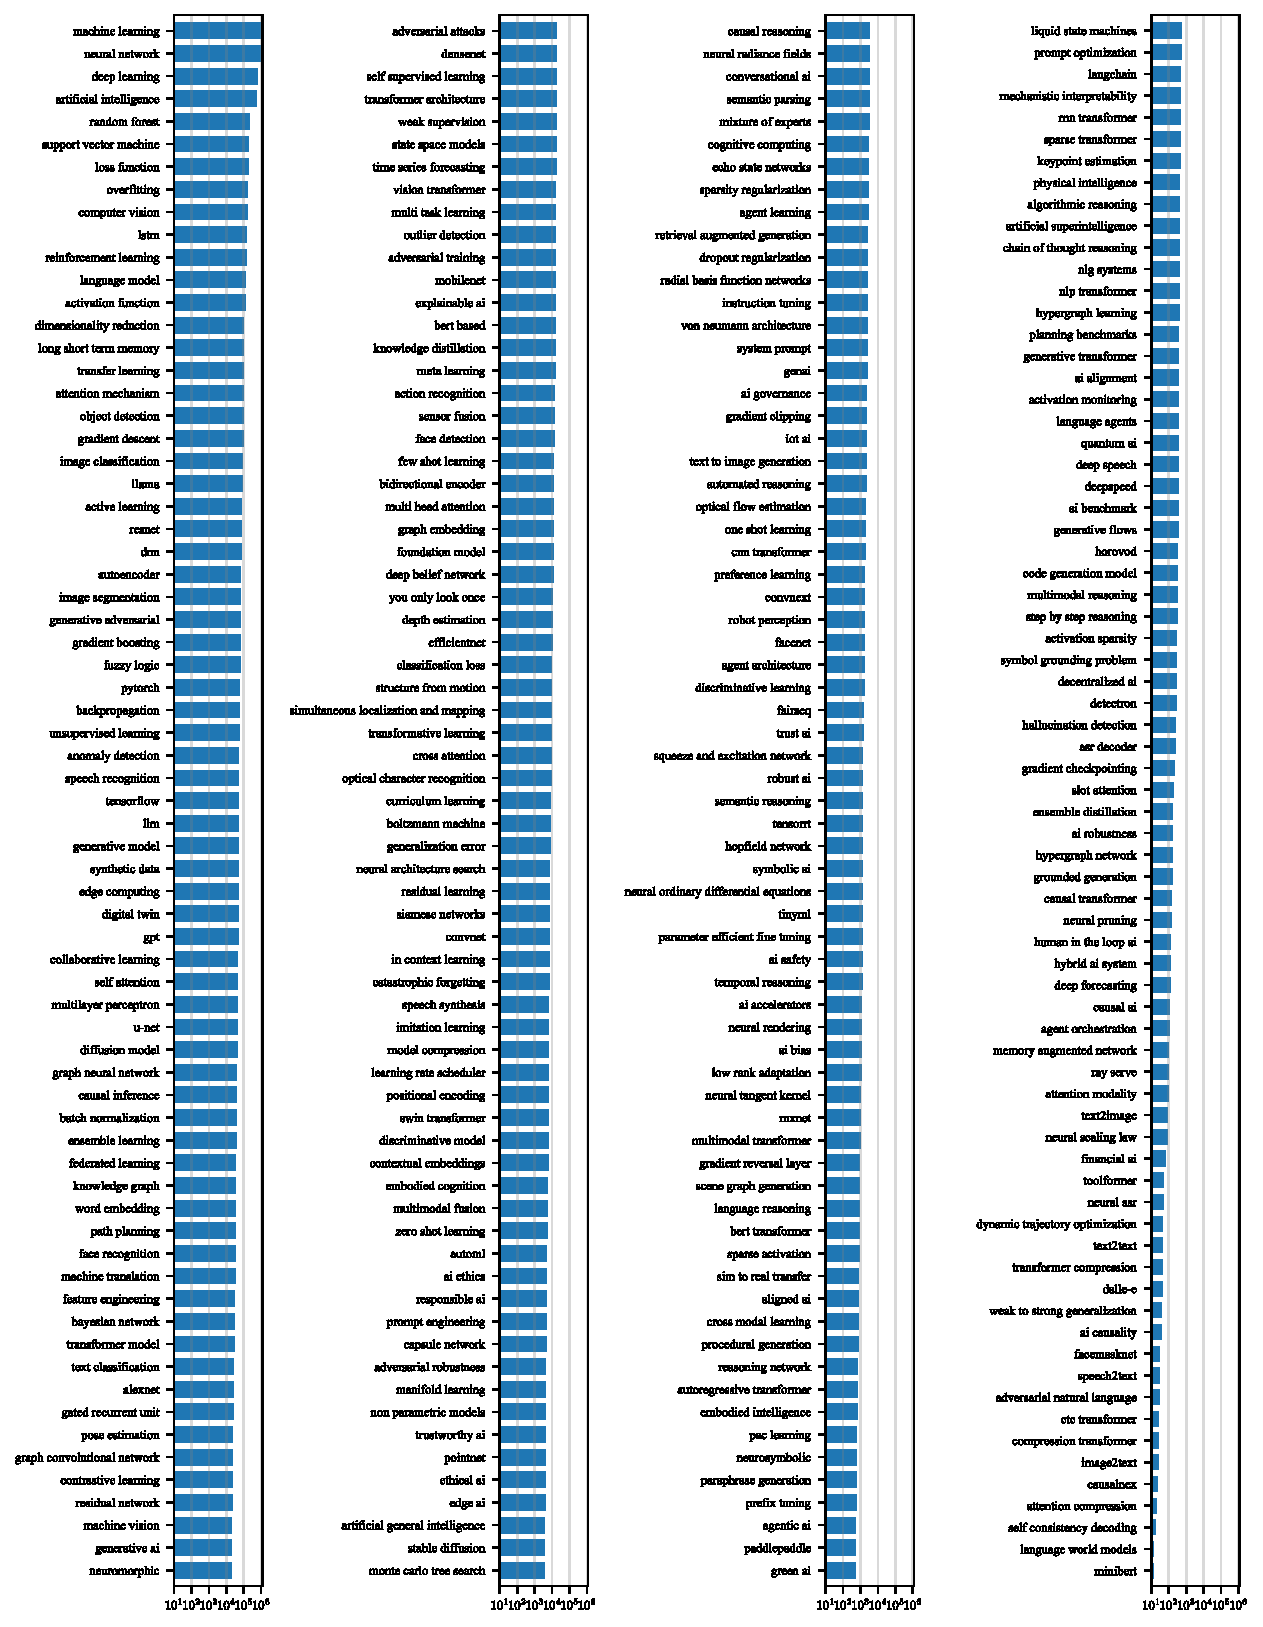
\includegraphics[height=0.95\textheight, keepaspectratio]{logarithmic_bar_graph_seach_term_document_count.pdf}
			\vspace{1em}
			\caption*{\small\textit{Figure 1 shows a sorted logarithmic bar graph of the retrieval counts for the 279 query terms used to construct the AI corpus from OpenAlex. Each bar represents the number of works returned by a hypothetical query with just that individual term. The fact that the total number of retrieved documents falls short of the sum of the individual term results is explained by the overlap inherent in the query design: Multiple search terms frequently co-occur in the title and the abstract of a single document.}}
			\label{fig:keyword_log_bar_graph}
		\end{center}
	}]
	
	
	
	
	\subsection{Quality Control and Postprocessing}
	\label{quality_control_and_postprocessing}
	
	Not all of the 3,346,705 records can contribute to the research questions. As already proposed in the \nameref{skg_selection}, each record must provide all of the following three datapoints: (i) An abstract for the topic modeling, (ii) a country of origin for geographic attribution, and (iii) at least one indicator for the estimation of research impact - either a numeric quantification of the incoming citations for the \nameref{fractional_citation_sum} or a list of the outgoing references for the \nameref{network_centrality}. In the following each of those three will be modified as individual features and filtered for completeness. First, \figurename~\ref{tab:metadata_completeness_initial_dataset} shows the metadata completeness of this initial dataset.
	
	\begin{figure}[H]
		\centering
		\caption{\textcolor{darkergray}{Metadata Completeness of Initial Dataset (\%)}}
		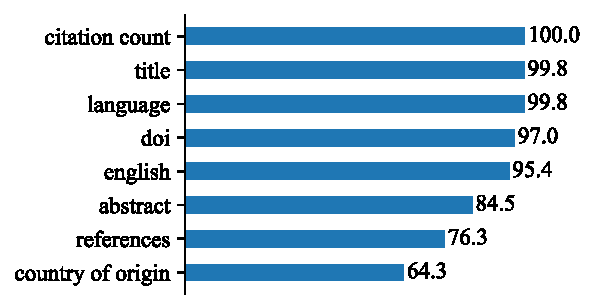
\includegraphics[width=\columnwidth]{resources/initial_dataset_completeness_clean.pdf}
		\vspace{-2em}
		\label{tab:metadata_completeness_initial_dataset}
	\end{figure}
	
	
	First is the filtering for the abstracts. 84.5\% of the publications have their abstracts recorded, but two additional quality rules are considered:
	\begin{enumerate}
		\item \textbf{Language Filter:} Due to the exclusive use of English search terms, an overwhelming majority of 95.36\% of the abstracts in the dataset are in English. The remaining 4.64\% (155,430 publications) were non-English, primarily Spanish (2.20\%), Indonesian (0.57\%), and Portuguese (0.41\%). This is the case only because even non-English abstracts use English words extensively.
		For reasons of technical feasibility and for the arguments already discussed in the introduction of the \nameref{dataset_extraction_pipeline_chapter}, filtering for English documents is carried out once again here.	
		\item \textbf{Length Normalization:} Abstracts with abnormally short or long abstracts were removed to ensure data consistency and reliability in downstream analysis. In total, 107,515 records with fewer than 100 or more than 1000 tokens were excluded. Such outliers were not filtered due to their length per se, but because unusually short or long abstracts might signal formatting or labeling errors.	
	\end{enumerate}
	
	Second is the publication's country of origin. Such a variable is not provided natively by OpenAlex but needs to be derived from the author's institutions. The extraction is based on two premises. First, that all publishing authors contribute the same fractional share to their publication and second that the authors' employing institutions are the best indicator for which national research body is represented (rather than publisher or funder). The resulting variable captures the geographic distribution of all contributing author institutions per work, represented as a list of tuples containing country codes and their respective shares of total author institutions adding up to 1. For example: \texttt{[("US": 0.75), ("DE": 0.25)]} indicates that 75\% of the authors work for institutions located in the US and 25\% in Germany. This variable could only be derived from 64.3\% of the publications. Inferring national attributions ex post (based on language, funders, or publishers) would introduce unknown biases and again lead to completeness bottlenecks not much smaller than the author's institution. Therefore, records without a country attribution from the author's institution were removed.
	
	Finally the research impact metrics are looked at. Outgoing references show a completeness of 76.3\%, yet publications missing them must not be filtered, because each record contributes a citation count and is thus already of use in assessing research impact.
	
	Beyond those three essentials there were no exclusions. Even missing DOI or title did not trigger an exclusion if the other criteria were satisfied. That is possible, because the problem of unique assignment and identification is solved by OpenAlex's internal ID. After applying the filtering, the final AI corpus comprises 1,986,659 publications of which 81.4\% are articles, 11.1\% preprints, 3.7\% reviews, 1.6\% book-chapters, 1.7\% peer-reviews, 0.5\% dataset and 0.2\% dissertations.
	
	
	\begin{figure}[H]
		\centering
		\caption{\textcolor{darkergray}{Metadata Completeness of Final Dataset (\%)}} % optional
		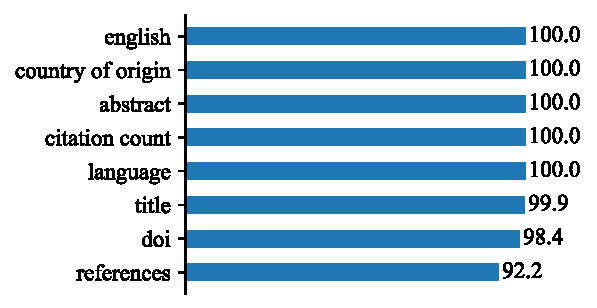
\includegraphics[width=\columnwidth]{resources/final_dataset_completeness_clean.pdf}
		\vspace{-2em}
		\label{tab:metadata_completeness_wokring_dataset}
	\end{figure}
	
	As shown by \figurename~\ref{tab:metadata_completeness_wokring_dataset}, the completeness of metadata is strongly correlated across fields, which means that the applied filtering has also resulted in the improvement of the completeness of all other metadata. That can best be seen from the references, whose completeness has improved from 64.3\% to 92.2\%.  Technically there will be methods that require references and thus publications without that variable won't contribute - for example in the construction of the \nameref{institution_network}. Beyond that, this dataset is considered complete and will not be manipulated or additionally filtered throughout the downstream analysis.
	
	
	\twocolumn[{%
		\begin{center}
			\vspace{-1em}
			\captionof{figure}{Dataset Construction Pipeline Diagram\\\vspace{1.5em}}
			\vspace{1em}
			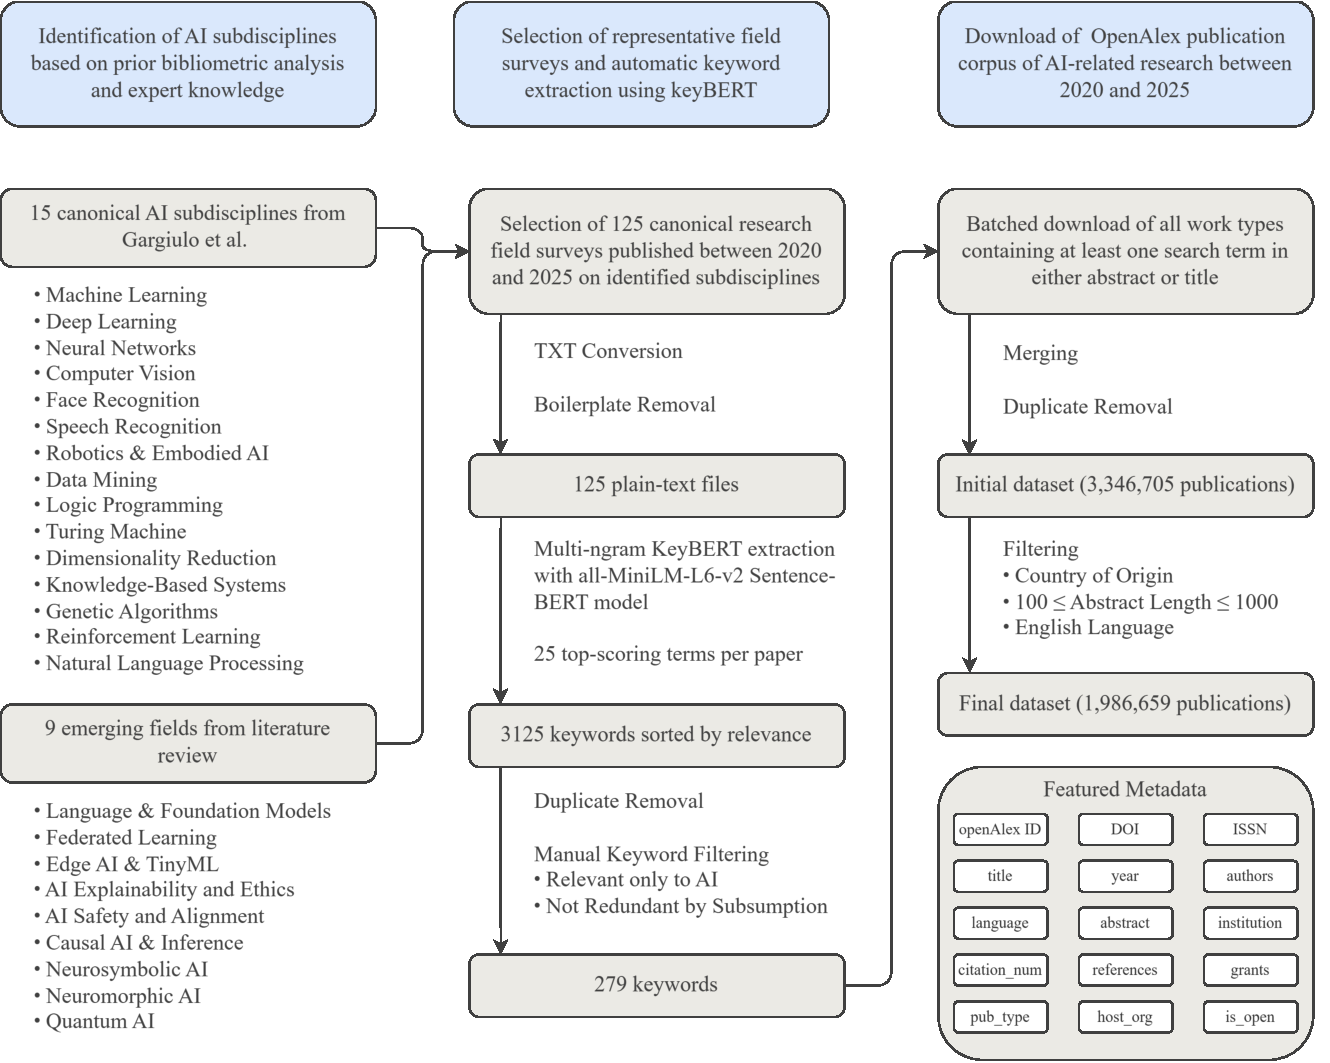
\includegraphics[width=\linewidth]{data_extraction_pipeline_diagram.pdf}
			\label{dataset_construction_pipeline_diagram}
			\vspace{3em}
		\end{center}
	}]
	
	
	
	
	\section{Method}
	
	With the finalized dataset in place, the next step is to determine how it can most effectively be interrogated to address the formulated research gap. Just like the research questions, the methodological framework consists of two complementary domains, each directly aligned with one of the central analytical objectives. First, the internal structure of AI research must be mapped out. Since we want to leave room for the dynamic field of AI research to surprise with unexpected subdisciplines, reusing the already presented taxonomies (Gargiulo et al. and OpenAlex) is not an option. Instead a semi-supervised hierarchical topic-modeling approach was chosen. It combines the rigor of an algorithmic discovery of even the smallest research fronts with the interpretability of a human-expert consolidation. Dense SPECTER embeddings capture the geometric structure of semantic similarity, and sparse TF-IDF features provide lexical vocabulary cues. These complementary representations form the basis for expert-guided cluster consolidation, through which latent subdisciplines within AI research are delineated.
	
	Second, the study assesses the relative research impact of individual countries within the subdisciplines identified in the first stage. While network-based indicators such as co-authorship or citation-graph centrality can in principle capture structural influence, they are heavily skewed by differences in collaboration cultures and institutional architectures. For this reason, the analysis emphasizes a simpler yet more robust indicator: The fractional citation sum.
	
	
	\subsection{Topic Modeling for Subdiscipline Retrieval}
	
	The structure of AI research investigated by \textbf{RQ1} requires the identification of subdisciplines. This task is particularly well-suited to topic modeling, as it can automatically discover latent thematic structures from large text corpora without relying on predefined categories, thereby capturing both established and emerging research areas in a data-driven manner. A topic modeling must begin with the translation of AI publications into a common semantic space in which they display machine-interpretable properties, and are thus rendered quantifiable in their differences and similarities. Clusters can then be defined based on the proximity and degree of internal cohesion. The desired number of subdisciplines, known as \textit{k}, is crucial for this step. Indicators such as the silhouette score or entropy-based algorithms are used to determine the optimal \textit{k}. They are intended to optimize cluster cohesion, for example by minimizing the sum of distances of all points to their closest centroids or by maximizing the distances between cluster edges, while simultaneously punishing increases in complexity (the size of \textit{k}). The results of these calculations have shown that no natural number of clusters emerges from the dataset. \textit{k} can be incremented to the point of semantic irrelevance and still continue to maximize cluster cohesion. In the silhouette score, this manifests in the absence of an elbow point - an abrupt flattening of the cohesion gains compared to the number of clusters. In entropy-based systems, which already include the penalty term, this is reflected in a plateau that is only subjected to random fluctuations. These findings are not entirely surprising,  but they resonate with broader concerns that data-driven heuristics for determining an optimal \textit{k} are often unstable and prone to post-hoc rationalization \cite{bulatov2024determination}. Since linguistic corpora inherently reflect human and disciplinary conventions rather than discrete natural boundaries a strategy that maximizes the strengths of bottom-up algorithmic discovery and top-down human supervision was applied. To achieve this, an initial \textit{k} is set to an excessively high size of 50 to ensure that small, semantically distinct clusters remain intact and are not merged into larger ones. A human expert then consolidates these 50 clusters into fewer and thus broader super-clusters. The expert's decision is based on two types of advice: An interactive semantic mapping that displays the topological relationships of the clusters and a lexical advice provided by the most representative vocabulary. The clustering and consolidation is performed in hierarchical iteration until the desired granularity is reached.
	
	
	More technically, the overall procedure consists of six steps:
	
	(i) The vectorization of texts into a numerical representation.
	
	(ii) The granular K-Means clustering.
	
	(iii) The identification of TF-IDF vocabulary.
	
	(iv) The expert-guided consolidation.
	
	(v) The repetition of the previous until sufficient granularity is reached.
	
	(vi) The propagation of cluster labels to the entire dataset. 
	
	In the following, each of them is described in their technical details.
	
	\subsubsection{SPECTER Vectorization}
	
	To transform the corpus into numerical representations that render its internal structure accessible to algorithmic interpretation, the SPECTER model is employed. This transformer-based encoder is trained on scientific citation networks to generate dense semantic embeddings of papers from their titles and abstracts \cite{cohan2020specter}. Each document is thus represented by a concatenation of its title and abstract. No stop-word removal is applied, since SPECTER is trained on natural language and thus benefits from full lexical context. Each concatenated text is tokenized into overlapping windows of 100 (stride of 50), and the resulting chunk embeddings are averaged to produce a single 768-dimensional vector per publication.
	
	
	\subsubsection{K-Means Clustering}
	
	Once documents have been vectorized, the next step is to identify semantically coherent groups of publications. For that purpose a clustering is performed using the K-Means algorithm on the SPECTER embedding space. Prior to clustering, all vectors are L2-normalized so that Euclidean distance approximates cosine similarity, ensuring that cluster assignments reflect angular proximity in the semantic space. K-Means iteratively minimizes the within-cluster sum of squared distances between documents and their respective centroids. Since it is to be expected that the publication volume of different clusters will vary considerably, there is a risk that small clusters will be assigned to their larger neighbors despite their within-cluster coherence and cross-cluster distinctiveness. Since these clusters could not be restored even by the human-in-the-loop design element, algorithmic clustering deliberately uses oversegmentation with a \textit{k} of 50.
	
	
	\subsubsection{TF-IDF Vocabulary}
	
	After the clustering stage, a sparse lexical representation is constructed for each of the 50 clusters using scikit-learn's \texttt{TfidfVectorizer} \cite{pedregosa2011scikit}. TF-IDF is part of the standard repertoire of natural language processing (NLP) and measures word importance as the product of two complementary functions: The \textit{representativeness} and the \textit{distinctiveness}. A word is representative of a publication if it occurs frequently within it, and distinctive for a publication if it occurs rarely outside of it. The TF-IDF analysis is performed separately for each cluster, whereas the reference documents required for the calculation of the \textit{distinctiveness} is sourced from the hierarchical siblings of the current topic modeling iteration. This ensures that the resulting vocabulary captures the most discriminative terminology within each semantic neighborhood, preserving distinctiveness as the analysis iteratively descends from broad domains to fine research fronts. The ten highest-scoring terms per cluster are selected as provisional descriptors, providing interpretable lexical signals that assist the human expert in consolidating the 50 fine-grained algorithmic clusters into coherent and semantically meaningful super-clusters.
	
	
	\subsubsection{Expert-Guided Cluster Consolidation}
	
	At this stage, each work in the dataset is assigned to one of 50 fine-grained clusters, and each cluster is characterized by a set of ten TF-IDF keywords. Based on these characteristics, an interactive visualization tool is created to support expert interpretation and consolidation. The interface renders the SPECTER embedding space in two dimensions using a uniform manifold approximation projection (UMAP) and provides dynamic functionality for toggling clusters on and off, zooming into local regions, and inspection of hover tooltips that display the associated TF-IDF terms. This combination offers the human expert (the author) two complementary semantic perspectives: A \textit{map} of the corpus' topological structure and a \textit{lexicon} of its contents. Using these two sets of cues, the expert consolidates the initially over-segmented clusters into a smaller number of semantically coherent super-clusters. Clusters that represent variations of a research field considered reasonably coherent are merged, while small but distinctive ones are preserved to avoid the loss of emerging or highly specialized subdisciplines. From this consolidation, a deterministic remapping is produced that assigns each of the 50 original cluster identifiers to its corresponding expert-defined super-cluster. All documents in the dataset are then relabeled according to this mapping, inheriting the super-cluster assignment of their respective K-Means cluster. To maintain a consistent, machine-readable representation, only numerical codes are used for the super-clusters, and these codes are stored directly in the SQLite database for downstream analysis. Finally, each consolidated super-cluster receives a non-numerical name determined by the expert based on its dominant themes, representative works, and recurring TF-IDF terminology. These names function as human-readable identifiers that capture the conceptual core of each super-cluster. They are interpretive approximations rather than mutually exclusive and jointly exhaustive categories. Overlaps and thematic continuities are thus expected and reflect the very nature of any research taxonomy.
	
	
	\subsubsection{Hierarchical Iteration}
	
	The clustering and consolidation procedure described above is not performed only once but repeated in a hierarchical manner. After the initial run, which partitions the entire corpus into a small number of broad research domains (from now on referred to as \textit{macro}), each resulting super-cluster is taken as a new input space and subjected to the same sequence of steps: Vectorization, high-\textit{k} clustering, TF-IDF labeling, interactive visualization, and expert consolidation. This second iteration produces a more fine-grained partition of each domain into thematic subfields (\textit{meso}). The process is then applied a third time within each meso-cluster, yielding fine-grained research fronts (\textit{micro}). This recursive application creates a consistent three-level hierarchy of subdisciplines. Since no cluster is subdivided into more than ten sub-clusters by the subsequent level, it is possible to use a single-digit number as an identifier for each iteration of the topic modeling. This means that the macro-clusters have consecutive single-digit numbers (starting with 0). The meso-clusters are described by two-digit identifiers, with the first digit being inherited from the parent cluster. The micro-cluster accordingly inherits the two digits of its meso-parent and adds a third digit itself. The hierarchical design enables analysis at multiple resolutions, from high-level disciplinary comparisons down to the granularity of individual research fronts.
	
	\subsubsection{Scaling Topics to the Full Dataset}
	
	Clustering the entire corpus of nearly two million works is very computationally expensive. To make the procedure more practical, the clustering was applied to a random subsample of 100,000 publications. This reduction preserves the topological and lexical relationships of the dataset while keeping resource requirements manageable. But it raises the challenge of how to extend the expert-defined super-clusters obtained from the subsample to the complete corpus. To address this, a reference set was constructed for each of the 50 initial K-Means clusters. Specifically, 200 \textit{central} abstracts (closest to the cluster centroid in embedding space) and 1000 \textit{random} abstracts were extracted per cluster. Once expert consolidation had been completed on the subsample, the reference embeddings were used to propagate labels to all 1,986,659 publications. Each document in the full corpus was embedded with SPECTER and assigned to the most similar item in the reference set by cosine similarity. Through this mechanism, every work in the dataset could be attributed to one of the predefined 50 clusters and, via the remapping, to its corresponding super-cluster.
	
	
	
	\twocolumn[{%
		\begin{center}
			\captionof{figure}{Topic Modeling Pipeline Diagram}
			\vspace{1em}
			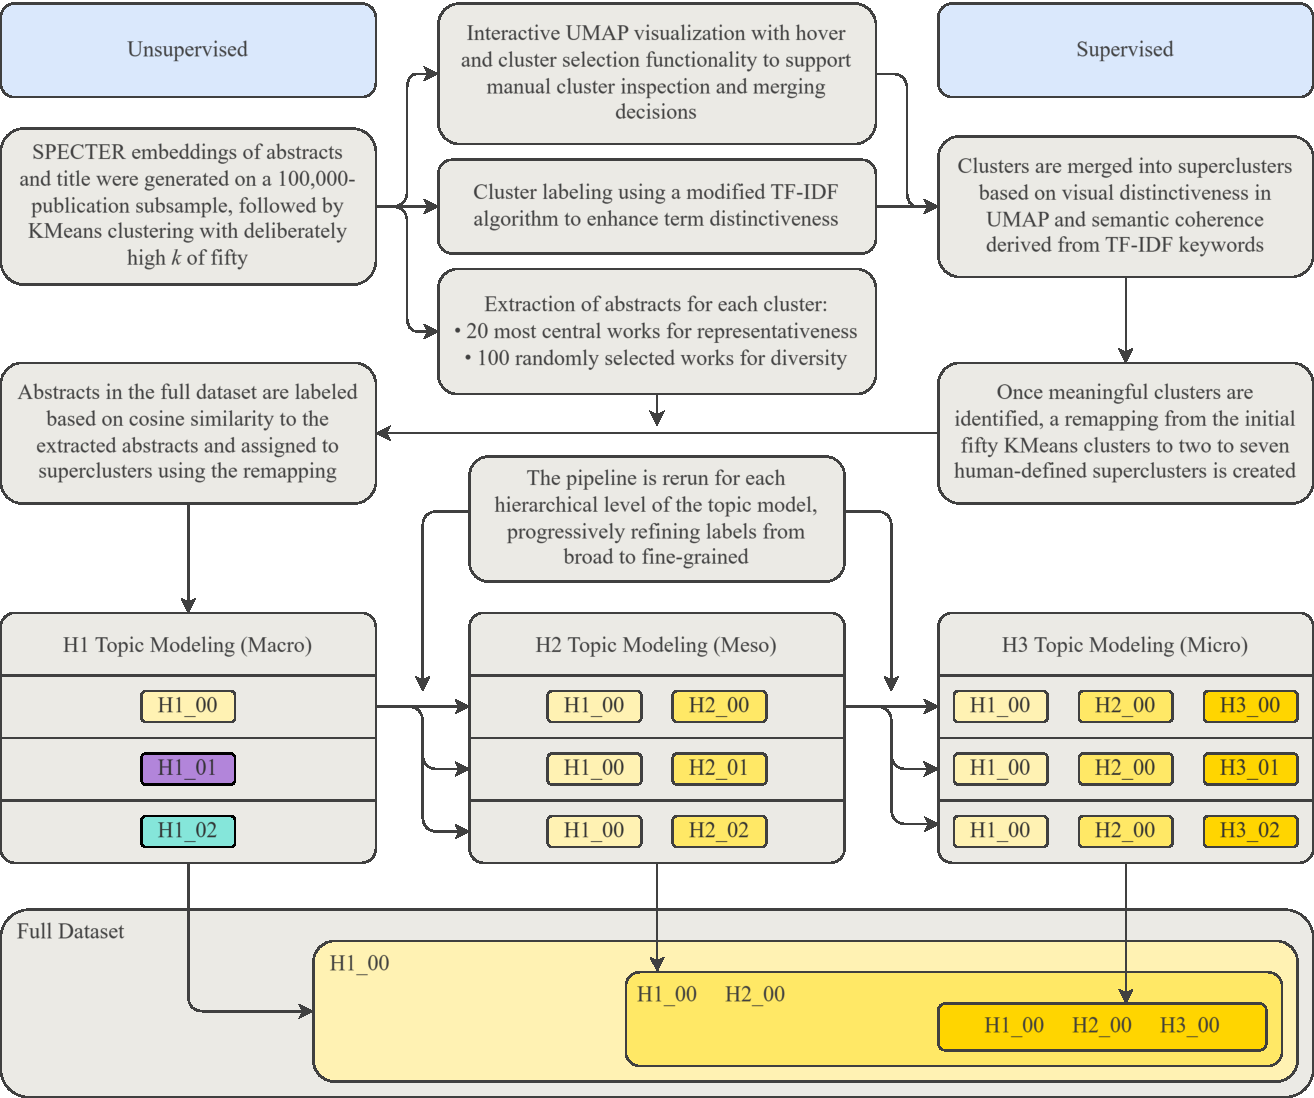
\includegraphics[width=\linewidth]{topic_modeling_pipeline_diagram_clean.pdf}
			\label{topic_modeling_pipeline_diagram}
			\vspace{3em}
		\end{center}
	}]
	
	
	
	
	\subsection{Assessment of Research Impact}
	\label{national_reserach_authority}
	
	The central aim of \textbf{RQ2} is to measure the geographic distribution of AI research impact across the globe. This question requires two specifications: First, it is necessary to clarify what is meant when referring to the globe - or more precisely, the granularity of the observed entities must be defined. Second, the examined research impact must be operationalized. The challenges associated with the specification of the entity granularity are already evident in the preceding research review. Most papers compared the US, China, and the EU, which are entities of different granularities. In order to universalize this European privilege, other IGOs are included in the comparison. Due to the limited space available for data visualization, no claim to completeness can be made, and given the diversity of structural characteristics, no uniform selection criteria can be presented. Instead, the selected IGOs can either be seen as political entities due to their political cohesion, or they are considered for their capacity to represent geographic regions. The dual nature of this selection mechanism can be tolerated once it is recognized that this study is not about creating a national ranking of AI capacities in order to attest any nation's superiority or backwardness. Rather it offers an exploratory observation that focuses on both political and geographical entities without confusing them as competitors. With this caveat, a list of eight selected IGOs and their membership count as of July 2025 is presented:
	
	
	\begin{enumerate}
		\item \textbf{The European Union (27 Members):} The EU must not be left out of any geo-economic comparison and is recognized as a powerhouse of research across all domains. More specifically, the EU has comprehensive supranational competencies and has already taken the first steps toward harmonizing the regulation and governance of AI with the \textit{Artificial Intelligence Act}.
		\item \textbf{The African Union (54):} Although the degree of regional integration has not yet reached the threshold of decision-making without total unanimity, it is worth considering one of the world's fastest-growing regions in terms of population and economy.
		\item  \textbf{The Association of Southeast Asian Nations (10):} ASEAN is also one of the traditional representatives of regional integration and is today regarded as a driver of growth and an integral part of the global value chain.
		\item \textbf{The Southern Common Market (5):} Mercosur represents nearly 300 million people from Latin America and is looked at for cross-regional comparison.
		\item \textbf{Gulf Cooperation Council (6):} In an attempt to diversify out of their extractive economy, members of the GCC are investing heavily in the sports and culture industries, digital startups, and advances in R\&D.
		\item \textbf{BRICS+ (10):} The BRICS countries are widely regarded as an umbrella organization for emerging regional powers challenging the post-Soviet unipolar order led by the US. Internally, as of 2025, the BRICS countries are united only in their shared rejection of this order, without presenting a uniform political alternative.
		\item \textbf{OECD (38):} The OECD represents the 1.4 billion people whose political-economic regime type can be described as liberal democratic. The OECD is a more formal designation for what is often referred to as the \textit{West} or, in more recent years, as the \textit{Global North}.
		\item \textbf{The Group of 77 (134):} The G-77 is the counterpart to the OECD: Arguably it is the most comprehensive formation of countries in the \textit{Global South}. Since the nature of the distinction is not economic but socio-political, no objective standards can be applied and assignments may change with the transition of power. Note that these IGOs do not partition the world into two fully discrete blocs - 21 countries (including several post-Soviet, island, and micro-states) are members of neither, and three countries (Chile, Colombia, and Costa Rica) hold dual membership.
	\end{enumerate}
	
	
	In subsequent analysis there are three lists of observed entities: (i) The 193 countries recognized by the United Nations, (ii) the eight IGOs, and (iii) the blocs (China, USA, EU-27). Now that it has been clarified which entities are to be investigated, it must be clarified which methods are suitable for measuring research impact. Such assessments can be fundamentally differentiated into those that work on a per-paper basis and thus highlight AI high-performers regardless of geoeconomic clout while other methods track entities' shares of the global AI dataset and thereby focus on the major economies disregarding ambitious \textit{small states}. For both perspectives several quantitative metrics exist to capture such qualities, but their suitability depends strongly on cross-entity data comparability. In the following three methods that are compatible with the affordances of the dataset are presented.
	
	\subsubsection{Network Centrality}
	\label{network_centrality}
	
	The measurement of network centralities is a specialty of scientometrics. It can be generated from two features of the OpenAlex dataset. From the list of outgoing references of each publication, which can be converted into an edge-list to generate a directed citation graph. And an undirected graph can be generated from the within-publication co-authorship. Both methods can be applied at all levels of granularity: For authors, institutions, and countries. Once such a graph has been generated, it provides topographical insights, such as neighborhoods, cluster sizes, densities, patterns, and outliers. While the topology itself is often determined by a priori parameterized algorithms such as ForceAtlas2, there is more leeway for decision-making when choosing the centrality metric. In the case of \textit{closeness centrality}, centrality is understood as the average minimum number of nodes that lie between a node and all others. The \textit{eigenvector centrality} is understood as the measure in which the centrality of a node is aggregated by the number of its direct connections and, by extension, their connections - central nodes not only have many direct neighbors themselves, but their neighbors also have many neighbors. Finally, a third popular method is the \textit{PageRank}, which measures the centrality of a node based on the probability of ending up at that node when randomly traversing the network. Despite the popularity and thus extensive research into these methods, their interpretability is severely limited in the case of the present dataset. This is mainly due to systematic differences in procedural conventions, such as the average number of authors per paper or the relative frequency of cross-institutional collaborations. To understand exactly how these two factors affect the presented centrality metrics, more can be found in the introductionary caveats of the \nameref{institution_network}. Due to the problem of uncertainty surrounding these systematic differences, centrality is used only once as a complementary method.
	
	
	\subsubsection{Field-Weighted Citation Impact}
	
	Another key metric in scientometrics is the FWCI. It normalizes the fractional citations sums of every publication against its publication year and field of research. In other words, each publication is standardized against the expected value of its peers. Fractional citation means that for each publication, the number of incoming citations is divided equally among the contributing authors and thus among the countries of origin of their institutions. The resulting number expresses the ratio of the actual citation counts to the expected citation counts. If the two are equal in size, the FWCI is 1. Fewer citations than the cohort average results in a number less than 1, and more citations results in a number greater than 1. The aim of the method is to prevent the disproportionate representation of an entity in older and strongly cited subdisciplines from having too strong an influence on the citation count, thereby overshadowing entities with a stronger focus on more recent papers from niche research areas. However, field-normalized metrics also introduce their own bias. Cohorts from younger and smaller research fields are particularly susceptible to outliers. Another possibility is a high average FWCI for an entity that focuses specifically on peripheral niches and is not represented at all in the citation-rich center - again, a suboptimal situation. These limitations are especially severe given that the topic modeling was not designed to harmonize cluster sizes and thus produced many small clusters exposed to FWCI fluctuations.
	
	
	\subsubsection{Fractional Citation Sum}
	\label{fractional_citation_sum}
	
	Finally, we come to fractional citation sums. As with the FWCI, each citation count is multiplied with each item of the publication's country of origin tuple and then added to their entity. Of all the methods of measuring research impact, this is the most straightforward, the most intuitive, and the most honest. This means that no further abstraction is applied. Citation sums do not attempt to identify the \textit{best possible} metric for representing influence among the many plausible candidates. This may lack precision, but at least it does not falsely suggest precision where there is none, and thus leaves researchers with the freedom to interpret the findings as they consider appropriate. This does not mean that this method is less biased, but it can be argued that biases are easier to find, to understand, and to criticize. Citation sums are one of the fundamentals of scientometric analysis, and their explanatory power is precisely defined. In addition, the citation count in the dataset is complete, while the outgoing references are missing for 7.8\% of the publications (with unknown bias). Whereas a range of different metrics are presented for measuring \nameref{impact_across_global_dataset}, citation sums are the dominant metric for determining \nameref{impact_across_subdisciplines}.
	
	\subsubsection{Explorative Applications}
	
	To properly analyze how research influence is spread across the identified AI subdisciplines, a basic frame of reference is needed. Since looking at country shares in individual fields without context wouldn't be very meaningful, we first need to figure out the following questions for countries, IGOs, and blocs in the monolithic AI dataset: (i) How many citations does each country contribute, how unevenly is research impact distributed globally, and how does it compare to the country's economic performance? (ii) What national performance profiles can be derived from the metadata in the dataset? (iii) How homogeneous or polarized is the distribution of citation counts within national research systems? (iv) Where are the most-cited institutions located, which cooperate with each other, and what structural clusters shape the global landscape?
	
	In order to establish such foundation, the methods introduced above - the fractional citation sum, the FWCI, and the network graph - are applied to the full dataset in a series of exploratory studies. These analyses are not primarily intended to test already existing hypotheses, but rather to map and systematically understand the collected material. Their goal is to develop a comprehensive basic understanding of global AI research dynamics through a multidimensional approach, which will serve as an interpretive framework for all subsequent, more granular findings. These sets of questions are operationalized as follows:
	
	1. \nameref{citation_geomapping}: The geomapping frames research performance within the global geopolitical and economic context by comparing citation sums with economic indicators.
	
	2. \nameref{performance_heatmap}: The multi-dimensional performance heatmap reveals complex national research profiles by simultaneously evaluating twelve quantitative indicators, moving beyond singular rankings to characterize research systems by their average citations, international collaboration, open-access share, growth rates, FWCI and others.
	
	3. \nameref{citation_percentile_distribution}: The analysis of citation percentiles benchmarks each country's publications against the global distribution, revealing which nations contribute proportionally to the most or least-cited publications.
	
	4. \nameref{institution_network}: The network analysis of the most-cited institutions breaks through the abstract level of national aggregates. It reveals the specific actors, their collaborative relationships, and the resulting academic clusters.
	
	Taken together, these exploratory analyses transform the raw dataset into an interpretative foundation. They establish the necessary baseline against which the subsequent discipline-specific strengths and weaknesses of the individual entities can be descriptively identified and interpreted.  To make things easier to understand, the implementations of these metrics, are detailed in the findings along with their specific applications.
	
	
	
	\section{Findings}
	\label{sec:findings}
	
	In the following, the synthesis of the compiled dataset and the methods derived from the research interests is conducted. This is done in the sequence of the research questions. \textbf{RQ1} is addressed by presenting the hierarchical clustering of the AI corpus: From broad domains to fine-grained research fronts, visualized through projections that highlight cluster cohesion and their relative positions in the research landscape. Then \textbf{RQ2} shifts the focus to the geopolitical dimension: Research impact is first assessed on the global dataset and then within the identified subdisciplines.
	
	\subsection{Hierarchical Topic Modeling}
	\label{sec:results_topic_modeling}
	
	To develop an understanding of the hierarchical structure and the decision-making process of the expert consolidation within the topic modeling, an exemplar clustering path based on topological and lexical cues is illustrated. After that, the identified clusters are presented and analyzed for their publication volume and growth trajectories at the macro and meso-level. Finally, all hierarchies are represented in a \textit{semantic landscape} whose density-based cluster summarizations delineate local neighborhoods and boundaries, providing a topological overview of semantic proximities among micro-clusters. Together, these three views establish the taxonomy, scale, dynamics, and geometry of AI research that the subsequent assessment of the research impact builds upon.
	
	Throughout the course of the findings, whenever clusters identified by topic modeling are discussed, the typewriter font and a color-coded identifier are used as shown in the following example: \textbf{\texttt{International Politics \& Law}} \microS{220}. This not only makes it possible to determine whether clusters or the research field itself are being discussed, but also provides two additional insights: First, the color scheme, which is also used in all subsequent graphs, indicates the macro-cluster. \microC{\textit{Purple}} stands for computer science, \microH{\textit{Blue}} for health science, \microS{\textit{Teal}} for social science, \microN{\textit{Yellow}} for natural science, and \microE{\textit{Orange}} for engineering. Second, the number of digits in the identifier reveals the hierarchy of the topic modeling in which the cluster in question is located. Single-digit IDs are reserved for macro-clusters, two digits are used for meso-clusters, and three digits are required for the most granular micro-clusters. That way, it can be avoided to repeatedly attribute clusters to their parents and hierarchical layers.
	
	\subsubsection{Exemplar Clustering Path}
	\label{exemplar_clustering_path_section}
	
	The hierarchical topic modeling procedure yielded five macro-clusters, comprising 31 meso-clusters and a total of 106 micro-clusters. These layers form a strict treemap-like hierarchy with unbroken parent-child relationships: Every micro-cluster belongs to exactly one meso-cluster and, through it, to a unique macro-cluster. Conversely, each macro-cluster is composed solely of its subordinate meso and micro-clusters, ensuring a consistent and exhaustive taxonomy without generational jumps. The following section illustrates the identification of one of these 106 micro-clusters as an exemplary case. Instead of the unrefined baseline configuration used in the interactive UMAP of the expert consolidation process, \figurename~\ref{fig:exemplar_clustering_hierarchy} employs a cluster summarization approach that enhances visual coherence for interpretive purposes. Here, each initial scatter of individual data points - often diffuse and irregular - is approximated as a polygon derived from a kernel density estimation. Assuming a normal distribution of points, the smallest possible contour enclosing 80\% of the individual publication vectors is extracted. While preserving semantic proximities, this method does inflate more loosely scattered clusters or put diffrently, underrepresents more dense clusters when considered against their publication volume. Interestingly its especially clusters of the most central computer science domain that suffer from that underrepresentation while more peripheral meso and micro-clusters are more prone to a wider spread and are thus inflated in size. Beyond those topological cues, every cluster is also characterized by its TF-IDF vocabulary, which identifies the most representative and distinctive terms of the cluster’s content when contrasted against its direct siblings. Together, the geometric UMAP representation and the TF-IDF term profiles provide two complementary interpretive lenses that pave the way for the human-in-the-loop consolidation process and enable a reconstruction of how local research fronts emerge within the broader taxonomy of AI research.
	
	As can be seen from \figurename~\ref{fig:exemplar_clustering_hierarchy}, each hierarchy of the topic modeling was consolidated to split its corpus into at least two and at most seven sub-clusters. The first iteration of the topic modeling divided the global dataset into five foundational domains of research. Computer Science occupies the center of the UMAP as it contains publications on core methods and concepts of AI, while the other four domains represent field-specific implementations whose vocabularies are only partly related to AI. The further they reach toward the periphery, the smaller the relative importance of AI within the cluster. The criterion of distinction for this central cluster was whether the ten highest-ranking TF-IDF terms were purely methodological and technical in nature, or already attributable to another domain of research. The terms of \texttt{\textbf{Health Science}} \microH{1} in the exemplar path are clearly indicative of the health domain with not a single term overlapping with the AI searchterms. Technical terminology such as \textit{computer vision}, \textit{classification}, \textit{segmentation}, and others indicative of disease detection are absent because, while central, they are not unique to the health domain. Terms such as \textit{patient}, \textit{cell}, and \textit{cancer}, on the other hand, are domain-specific and therefore, even a paper that is largely about the implementation of AI yet performs, for example, cancer detection would be labeled \textbf{\texttt{Health Science}} \microH{1} in the macro-level topic modeling.
	
	\twocolumn[{%
		\begin{center}
			\captionof{figure}{Exemplar Clustering Path across three Hierarchies}
			\vspace{1em}
			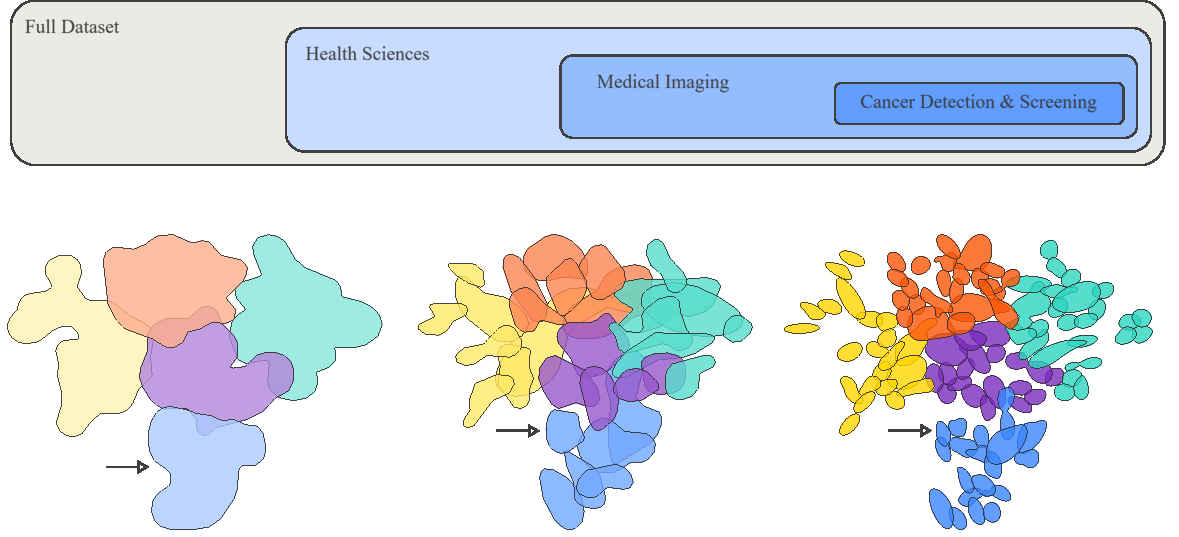
\includegraphics[width=\linewidth]{resources/exemplar_clustering_hierarchies_cancer_detection_clean_002.pdf}
			\vspace{1.5em}
			
			{\small
				\color{darkgray}
				\setlength{\tabcolsep}{8pt}
				\renewcommand{\arraystretch}{1.15}
				\begin{tabular*}{\textwidth}{@{\extracolsep{\fill}\hspace{6em}} l @{\hspace{1.4em}} l @{\hspace{1.0em}} l @{\hspace{6em}\extracolsep{\fill}}}
					\toprule
					\multicolumn{1}{c}{\hspace{4em}\shortstack{\textbf{\texttt{Health Sciences }}} \microH{1}} &
					\multicolumn{1}{c}{\shortstack{\textbf{\texttt{Medical Imaging }}} \microH{10}} &
					\multicolumn{1}{c}{\hspace{-6em}\shortstack{\textbf{\texttt{Cancer Detection }} \microH{102}}\hspace{-3em}} \\
					\midrule
					1\, patient & 1\, image & 1\, tumor \\
					2\, cell & 2\, segmentation & 2\, cancer \\
					3\, cancer & 3\, deep & 3\, breast \\
					4\, disease & 4\, detection & 4\, brain \\
					5\, clinical & 5\, propose & 5\, segmentation \\
					6\, protein & 6\, network & 6\, feature \\
					7\, gene & 7\, classification & 7\, mri \\
					8\, brain & 8\, learn & 8\, classification \\
					9\, treatment & 9\, cnn & 9\, liver \\
					10\, tumor & 10\, medical & 10\, prostate \\
					\bottomrule
				\end{tabular*}
			}
			
			\vspace{1.5em}
			\caption*{\small\textit{Figure 6 Illustrates a single path through the three-level hierarchical topic modeling from macro-domain to micro-cluster. The numbered tables list the top-10 TF-IDF terms calculated for each level and served as lexical cues alongside the UMAP projection of SPECTER embeddings during expert-guided consolidation of the initial high-k K-Means partition.}}
			\label{fig:exemplar_clustering_hierarchy}
			\vspace{2em}
		\end{center}
	}]
	
	
	
	% \twocolumn[{%
		%	\begin{center}
			%		\vspace{-3em}
			%		\captionof{figure}{Mesocluster UMAP}
			%		\vspace{1em}
			%		\includegraphics[width=\linewidth]{resources/100k_mesocluster_visulization_greybox.pdf}
			%		\vspace{1em}
			%		\caption*{\small\textit{Explaination of why there is extensive 	overlapse, -> UMAP does that when projecting highdimensional data on 2D space and also clustering was done not only using UMAP clusterings but also the TFIDF Labels.}}
			%		\label{fig:mesocluster_umap_with_legend}
			%		\vspace{2em}
			%	\end{center}
		%}]
	
	Apart from \textbf{\texttt{Computer Science}} \microC{0} and \textbf{\texttt{Health Science}} \microH{1}, there are \textbf{\texttt{Social Science}} \microS{2}, \textbf{\texttt{Natural Science}} \microN{3} and \textbf{\texttt{Engineering}} \microE{4}. There is no universally accepted distinction for foundational scientific domains, and even if such a taxonomy existed, the K-Means clustering would not necessarily acknowledge it. Therefore, some adjustments were made to accommodate the proximities displayed in the embedding space. These include the attribution of a majority of mathematics-related works to \textbf{\texttt{Computer Science}} \microC{0}, despite the fact that they are largely considered part of the social sciences. Edge cases such as \textbf{\texttt{Cybersecurity \& Privacy}} \microE{40} (between \textbf{\texttt{Computer Science}} \microC{0} and \textbf{\texttt{Engineering}} \microE{4}) or \textbf{\texttt{Urban Development}} \microS{25} (between \textbf{\texttt{Social Science}} \microS{2} and \textbf{\texttt{Engineering}} \microE{4}) were arbitrarily assigned to one of the two domains to preserve their coherence as clusters at the meso-level.
	
	Observing the meso-cluster TF-IDF terms, it can be seen that medical terminology largely disappears. That means its role in creating distinction has been exhausted in the previous hierarchy. For the next hierarchy, the most distinctive characteristic of the exemplar cluster is its focus on visual data. From general terms like \textit{image} and operational vocabulary such as \textit{segmentation} and \textit{classification} to methodological descriptors like \textit{deep learning} (here tokenized and lemmatized) and \textit{CNN}, we find indicators differentiating \textbf{\texttt{Medical Imaging \& Radiology}} \microH{10} from its meso-siblings \textbf{\texttt{Neuroscience \& Mental Health}} \microH{11}, \textbf{\texttt{Molecular Biology \& Drug Discovery}} \microH{13} and \textbf{\texttt{Genetics \& Genomics}} \microH{15} - all of which do not primarily work on visual data.
	
	In the third and final hierarchy, \textbf{\texttt{Medical Imaging \& Radiology}} \microH{10} and all other meso-clusters are subdivided again. Often this most granular clustering results in well-defined and highly specific research fronts. In the case of the exemplar clustering path, the meso-cluster is split into four micro-clusters describing different applications of health-related viusal pattern recognition: \textbf{\texttt{Musculoskeletal Imaging}} \microH{100}, \textbf{\texttt{Neuroimaging \& Imaging Physics}} \microH{101}, the presented \textbf{\texttt{Cancer Detection \& Screening}} \microH{102}, and a somewhat residual micro-cluster termed \textbf{\texttt{Disease Diagnostics}} \microH{103}, which includes terminology from skin illnesses, organ physiology, and ophthalmology.
	
	The macro and meso-levels are not just necessary intermediate steps to arrive at the micro-cluster. All three levels of granularity contribute to the understanding of the field of AI research and are used depending on the intention of the respective subject. This often leads to a sequence of observation similar to the development process, starting with broad domains and then zooming in on the research fronts.
	
	
	\subsubsection{Publication Volume \& Growth}
	\label{cluster_size_meso_level}
	
	Now that an understanding of the clustering process has been established, a deeper look into the qualities of the resulting topics is possible. In the following a foundational assessment of scientific attention in the AI domian is performed by analyzing and comparing clusters' publication volumes and growth rates. The treemap presented in \nameref{cagr_stacked_bar_graph} shows the 31 meso-clusters structured by their parents horizontally and then displayed in stacked bar graphs. The box sizes thus express the overall publication volume of each meso-cluster while its colorization reflects the growth rates from 2020 to 2023. The final year 2024 was removed from the analysis because publications can take up to a year to be indexed by OpenAlex, and growth rates would thus be systematically underestimated. Growth rates are expressed as compound annual growth rates (CAGR), which calculate the difference between the start and the end of a period and assume uniform change across the span.
	
	The largest meso-cluster is \textbf{\texttt{Computer Vision \& Image Processing}} \microC{00}, covering 8.5\% of all publications, with its semantically adjacent medical relative \textbf{\texttt{Medical Imaging \& Radiology}} \microH{10} adding another 5.1\%. Their prominence is unsurprising: Both are located in mature incentive structures, with well-established application in industrial and clinical pipelines. Other sizable meso-clusters include \textbf{\texttt{Clinical Information \& Public Health}} \microH{12} with 6.0\%, \textbf{\texttt{Machine Learning Foundations}} \microC{04} with 5.9\%, and \textbf{\texttt{Business \& Management}} \microS{24} with 5.6\%, further endorsing the hypothesis of a correlation between publication volume and the existence of a developed market application rather than variables such as public attention. This point becomes especially visible when looking at the other end of publication volumes: \textbf{\texttt{Ethical \& Creative AI}} \microS{26} accounts for just 1.4\% of the corpus, and \textbf{\texttt{Politics \& Governance}} \microS{22} adds 1.3\%. This contrasts sharply with findings from a news corpus (sourced from 12 Western European and US-american outlets) where \textit{AI ethics and morality} alone covers 8.0\% of articles, \textit{public accountability} another 12.4\% and \textit{economic consequences} 13.1\% \cite{Zai2025Voices}. That means that taken together, more than a third of articles touch upon topics that make up only 2.7\% of publications in the OpenAlex corpus.
	
	Beyond the aggregated publication volume, the analysis provides the growth trajectory. One should keep in mind that this study is designed as a cross-sectional snapshot of the most recent scientific output and that the filtering required for the CAGR leaves only a four-year period. Therefore, the resulting growth rates are exposed to short-term fluctuations and outliers especially for the micro-level and clusters of small publication volumes. The publication CAGR of global academia measured by OpenAlex records is at -3.42\% in the observed periode. That means that 2023 is still trailing behind pre-pandemic 2020. In contrast, the AI corpus shows a growth rate of 22.15\% per year. But the aggregated CAGR masks substantial variation across the subdisciplines. At the macro-level, \textbf{\texttt{Computer Science}} \microC{0} grows at only 14.74\%, well below \textbf{\texttt{Health Sciences}} \microH{1} (22.59\%), \textbf{\texttt{Social Sciences}} \microS{2} (26.39\%), \textbf{\texttt{Natural Sciences}} \microN{3} (29.30\%) and \textbf{\texttt{Engineering}} \microE{4} (20.91\%). Those numbers suggest that research on more peripheral implementations of AI is expanding faster than the development of core methods. At the meso-level, some small clusters like \textbf{\texttt{Urban Development}} \microS{25} (45.61\%), \textbf{\texttt{Energy \& Thermodynamics}} \microN{32} (31.53\%), and \textbf{\texttt{Construction \& City Planning}} \microN{36} (31.96\%) show the expected volatility from low baselines. Yet larger and thus more stable meso-clusters such as \textbf{\texttt{Business \& Management}} \microS{24} (30.57\%), \textbf{\texttt{Material Science}} \microN{31} (31.83\%), and \textbf{\texttt{Agriculture \& Forestry}} \microN{33} (34.51\%) confirm the over-proportionate growth rates of fields traditionally more distant to AI. By contrast, core-method meso-clusters like \textbf{\texttt{Natural Language Processing}} \microC{01} (12.82\%), \textbf{\texttt{Machine Learning Foundations}} \microC{04} (8.27\%), and \textbf{\texttt{Robotics \& Mechatronics}} \microE{45} (12.12\%) are among the slowest growing. One explanation for this phenomenon argues for a general research-cycle from \textit{niche} over \textit{motor} and \textit{basic} to \textit{decline}: Once foundational methods mature, marginal returns to additional method papers fall, and accumulated know-how is increasingly mobilized downstream in domain applications \cite{Belfiore2022Characterising}. This is consistent with the hypothesis of AI behaving as a general-purpose technology which is diffusing across the sciences where the steepest growth appears at application frontiers that were historically farthest from AI.
	
	\twocolumn[{%
		\begin{center}
			\vspace{-3em}
			\captionof{figure}{Treemap of Meso-Clusters by Publication Count and Growth Rate}
			\vspace{1em}
			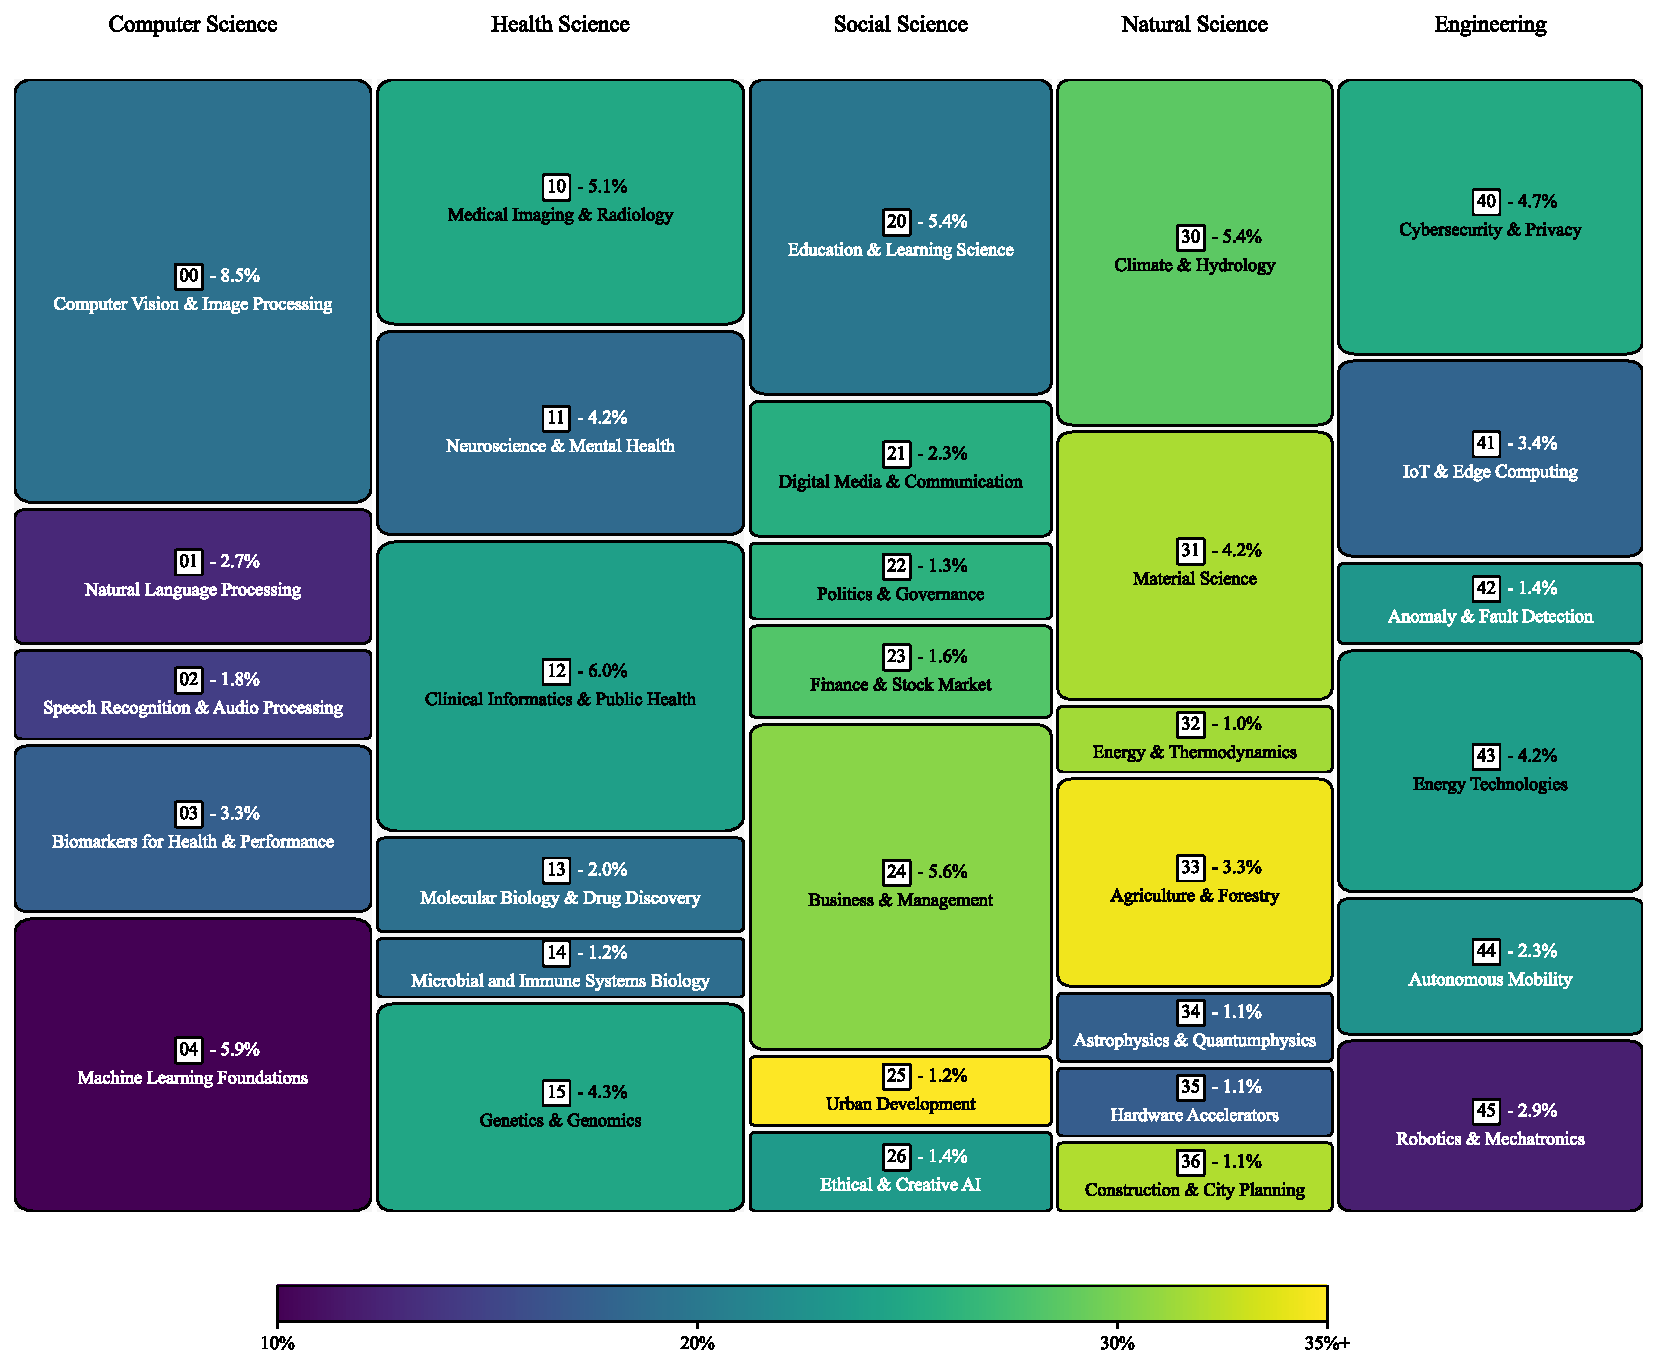
\includegraphics[width=\linewidth]{stacked_bars_h1_h2_cagr.pdf}
			\vspace{1em}
			\caption*{\small\textit{Figure 7 shows meso-cluster cells arranged horizontally by their macro-cluster and vertically by their numeric identifier. Cell size encodes total publication count aggregated over the full dataset, while the color scale encodes the growth rates measured as CAGR between 2020 and 2023. Data for 2024 are excluded from the analysis due to incomplete coverage on OpenAlex. 35\% CAGR was arbitrarily chosen as maximum of the color-scale.}}
			\label{cagr_stacked_bar_graph}
			\vspace{2em}
		\end{center}
	}]
	
	
	\subsubsection{Subdiscipline Landscape}
	\label{subdiscipline_landscape}
	
	Finally, the analysis zooms in to the micro-layer and shows how the research landscape looks at its most granular resolution. Just like in \nameref{exemplar_clustering_path_section},  \figurename~\ref{fig:cluster_summarization_umap} shows a UMAP with the density-based cluster-summarization. But this time all 106 micro-clusters are labeled and can be attributed to their parents and grandparents based on colorization and their numeric identifier. With the detailed subdiscipline landscape, a deeper observation of singular subdisciplines is possible. In the following each macro-cluster with their composing meso and micro-clusters is looked at and analyzed for their semantic relations in numerical order. The layout of the UMAP is inherently non-deterministic, meaning that the relative positioning of clusters may vary slightly across different runs. Nonetheless, repeated iterations have shown that the overall topology of the embedding space remains largely stable. What does change, however, is the rotation of the layout, which is entirely arbitrary and carries no analytical meaning. Despite this, cardinal directions are used in the following discussion as a convenient way for describing spatial relations within the presented UMAP.
	
	\textbf{\texttt{Computer Science}} \microC{0} builds the center of the graph. It is comprised of 5 meso-clusters and 18 micro-clusters. While already established as the largest meso-cluster in terms of publication volume, \textbf{\texttt{Computer Vision \& Image Processing}} \microC{00} exhibits comparatively small micro-clusters in the UMAP due to limited inner-cluster semantic spread. They are located at the south-western region of \textbf{\texttt{Computer Science}} \microC{0}, adjacent to \textbf{\texttt{Medical Imaging \& Radiology}} \microH{10} in the south and bordering \textbf{\texttt{Topography \& Earth Observation}} \microN{301} and \textbf{\texttt{Mobility \& City Planning}} \microN{361} in the west. While vastly different in their domains of application, all of these clusters share a common methodological foundation. The TF-IDF terms reveal that they are unified by similar operational logics such as \textit{segmentation} and \textit{classification}, and by methodological frameworks largely based on \textit{CNNs} and \textit{deep learning}. Whether publications from those clusters are dealing with traffic video footage, satellite imagery, or symptom diagnostic records, all of them employ related pattern recognition pipelines, resulting in a closely aligned technical vocabulary across their abstracts. Second there is \textbf{\texttt{Natural Language Processing}} \microC{01}, located along the eastern boundary of \textbf{\texttt{Computer Science}} \microC{0}, directly adjacent to \textbf{\texttt{Digital Media \& Communication}} \microS{21}. This proximity arises primarily from the shared focus on text as the principal input variable. While \textbf{\texttt{Computer Science}} \microC{0} emphasizes methodological vocabulary related to transformer architectures, knowledge graphs, and reasoning models, \textbf{\texttt{Social Science}} \microS{1} applies these techniques to research on social media communication, sentiment analysis, and content integrity classification. Right below lies \textbf{\texttt{Speech recognition \& Audio Processing}} \microC{02}. Situated in the border triangle of \textbf{\texttt{Computer Science}} \microC{0}, \textbf{\texttt{Health Science}} \microH{1} and \textbf{\texttt{Social Science}} \microS{2}, this meso-cluster includes \textbf{\texttt{Music \& Acoustic Modeling}} \microC{020} and \textbf{\texttt{Emotion \& Cognition in Audio}} \microC{021}. Its proximity to \textbf{\texttt{Health Science}} \microH{1} is somewhat surprising given that there is no independent micro-cluster like phoniatrics. However, the very fact that this field conceptualizes the human primarily as a physical entity, rather than merely as a source of digital traces, may account for the observed semantic proximity. In the central-southern area of \textbf{\texttt{Computer Science}} \microC{0} lies \textbf{\texttt{Biomarkers for Health \& Performance}} \microC{03}, a cluster whose thematic scope naturally borders \textbf{\texttt{Health Science}} \microH{1}.
	
	Although not exclusively focused on medical applications, it centers on the computational measurement and interpretation of biological signals, bridging algorithmic analysis with physiological observation. Finally, in the northern region of \textbf{\texttt{Computer Science}} \microC{0} lie some of the largest and most central micro-clusters. All six belong to \textbf{\texttt{Machine Learning Foundations}} \microC{04}, which accounts for 5.9\% of the total publication volume, yet their internal semantic spread causes them to occupy a disproportionately large area within the UMAP, far exceeding the space covered by the most-publishing \textbf{\texttt{Computer Vision \& Image Processing}} \microC{00}. \textbf{\texttt{SVM \& Decision Tree}} \microC{042} forms a bridge between \textbf{\texttt{Engineering}} \microE{4} and \textbf{\texttt{Natural Science}} \microN{3}, aligning particularly with \textbf{\texttt{Energy System Modeling}} \microE{433} and \textbf{\texttt{Construction Technology}} \microN{360} due to shared methodologies in predictive modeling of structural integrity, system failure, and cost optimization. On the northwestern boundary, \textbf{\texttt{Probabilistic Modeling}} \microC{043}, and \textbf{\texttt{Graph Learning \& Network Modeling}} \microC{045} connect with \textbf{\texttt{Task Scheduling \& Decision Making}} \microE{452}, and \textbf{\texttt{Game Theory \& Decision Making}} \microS{222}, reflecting overlaps in optimization and decision logic. At the very center, \textbf{\texttt{Neural Network Architectures}} \microC{041} occupys a vital position, underscoring two key characteristics: First, neural networks are relevant across a large share of the AI corpus, and second, a substantial body of research is dedicated not to implementation but to the optimization of learning architectures themselves.
	
	\textbf{\texttt{Health Science}} \microH{1} is the least dense of all macro-domains, comprising 6 meso-clusters and 19 micro-clusters. Beyond \textbf{\texttt{Medical Imaging \& Radiology}} \microH{10}, the most central meso-clusters include \textbf{\texttt{Neuroscience \& Mental Health}} \microH{11} and \textbf{\texttt{Clinical Informatics \& Public Health}} \microH{12}. The proximity of \textbf{\texttt{Clinical Informatics \& Public Health}} \microH{12} to \textbf{\texttt{Computer Science}} \microC{0} can be explained by AI’s application in the modeling of complex systems ranging from health infrastructure to pandemic diffusion. In contrast, the proximity of \textbf{\texttt{Neuroscience \& Mental Health}} \microH{11} requires a more cautious interpretation. The TF-IDF terms indicate a vast adoption of AI methods in this field, however, its centrality may also stem from the extensive lexical and conceptual borrowings of AI scholars from the study of biological cognition. Further south, three more peripheral meso-clusters can be identified: \textbf{\texttt{Molecular Biology \& Drug Discovery}} \microH{13}, \textbf{\texttt{Microbial \& Immune System Biology}} \microH{14}, and \textbf{\texttt{Genetics \& Genomics}} \microH{15}. In these fields, research is primarily driven by experimental and biochemical paradigms rather than computational ones, with AI serving only as a supplementary tool among a wide range of analytical techniques. This marginal methodological role is also illustrated by the absence of AI-specific terminology in the TF-IDF rankings. Consequently, their distance within the UMAP can be interpreted as a semantic manifestation of AI’s auxiliary rather than foundational function in these areas.
	
	With 7 meso-clusters and 25 micro-clusters, \textbf{\texttt{Social Sciences}} \microS{2} represents the most finely subdivided domain. In the western border region of \textbf{\texttt{Computer Science}} \microC{0}, \textbf{\texttt{Ethical \& Creative AI}} \microS{26} appears beyond the already discussed \textbf{\texttt{Digital Media \& Communication}} \microS{21}. Further north, and in close proximity to  \textbf{\texttt{Engineering}} \microE{4}, lies \textbf{\texttt{Business \& Management}} \microS{24}, which shares methodological paradigms such as risk assessment, manufacturing optimization, and performance measurement with classical engineering subdisciplines. Moving eastward, the focus departs from the material world and transitions into the metaphysical abstraction of \textbf{\texttt{Finance \& Stock Market}} \microS{23}.
	
	\twocolumn[{%
		\begin{center}
			\vspace{-3em}
			\captionof{figure}{Summarized UMAP and Taxonomy of AI Subdisciplines}
			\label{fig:cluster_summarization_umap}
			\vspace{1em}
			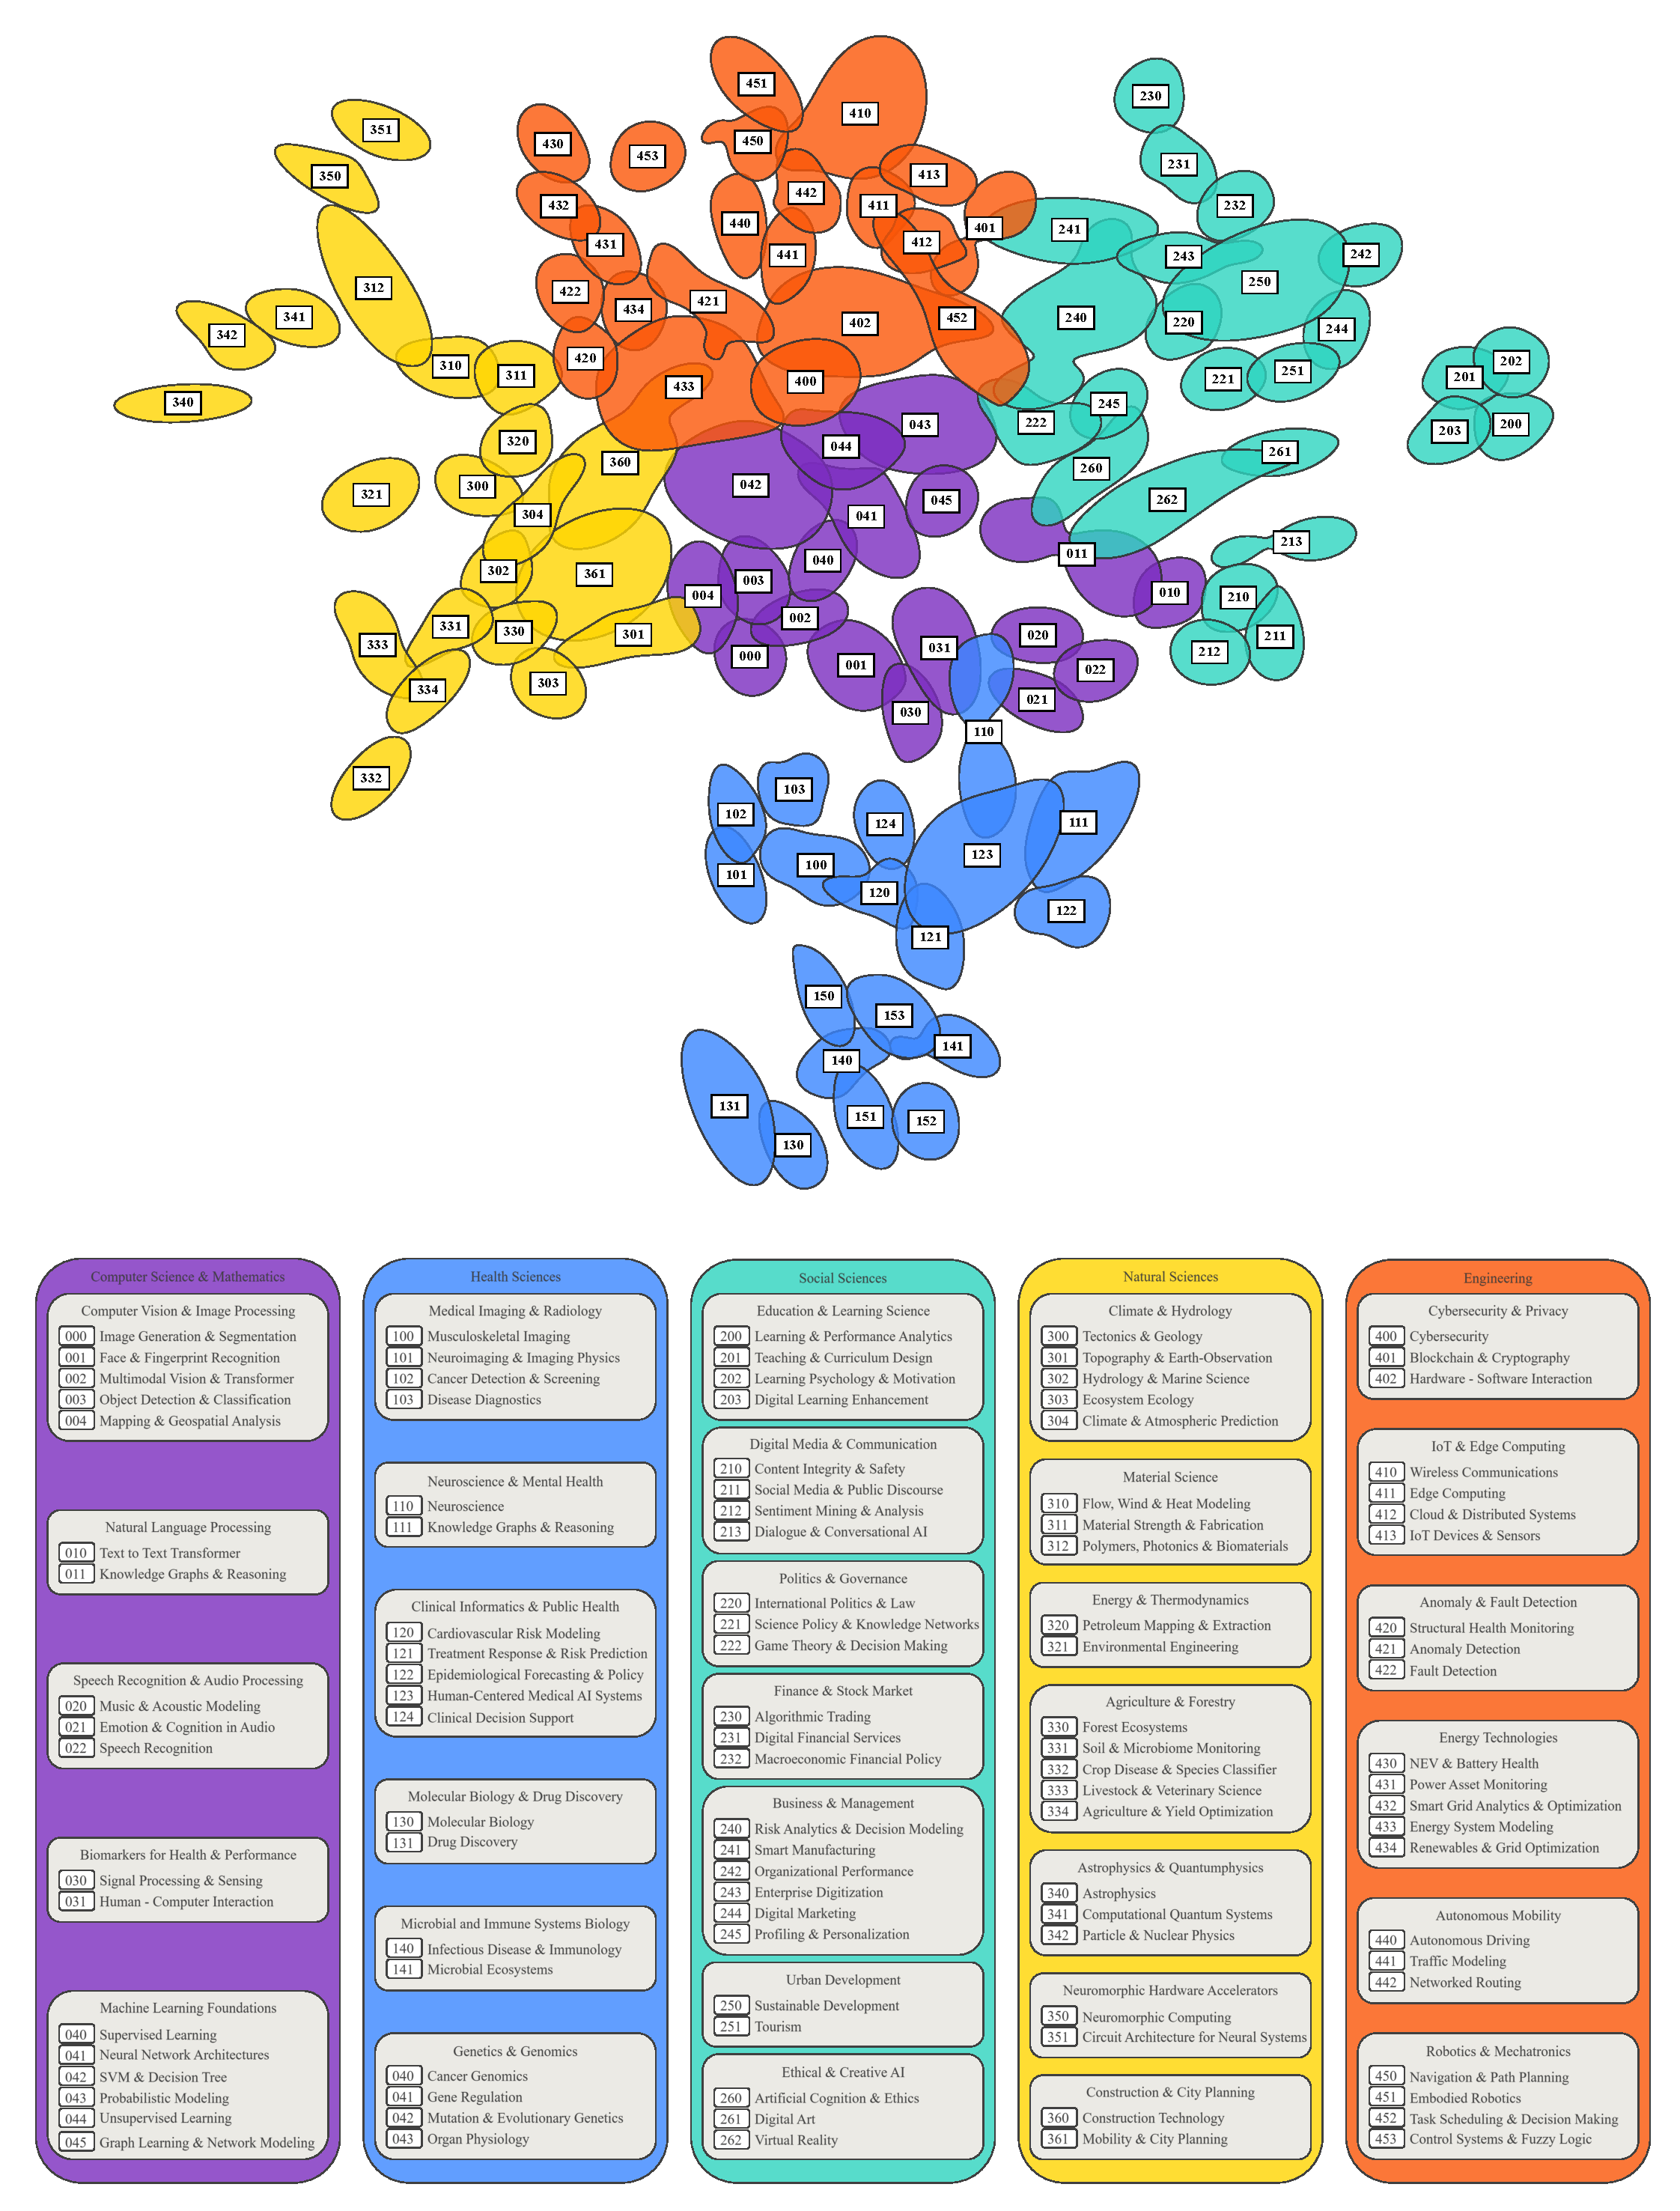
\includegraphics[width=\linewidth]{cluster_umap_with_legend_2025_10_09_bigger_clusters.pdf}
			\vspace{1em}
			\caption*{\small\textit{Figure 8 shows a density-summarized UMAP of the 106 micro-clusters identified in the SPECTER embedding space. Cluster sizes represent semantic spread, not publication volume.  Below there is a legend displaying the full taxonomy of the expert-consolidated clusters across the three hierarchies. }}
		\end{center}
	}]
	
	
	Directly below, \textbf{\texttt{Urban Development}} \microS{25} and \textbf{\texttt{Politics \& Governance}} \microS{22} can be found, with their \textbf{\texttt{Game Theory \& Decision Making}} \microS{222} forming a rare renegade micro-cluster closely aligned with \textbf{\texttt{Probabilistic Modeling}} \microC{043}. Along the eastern periphery of \textbf{\texttt{Social Science}} \microS{2}, \textbf{\texttt{Education \& Learning Science}} \microS{20} emerges. Its TF-IDF profile is dominated by pedagogical terminology such as \textit{student}, \textit{teacher}, and \textit{didactic}, which outweighs the methodological vocabulary typical of AI applications, illustrating a research orientation centered more on human learning processes than on algorithmic innovation.
	
	\textbf{\texttt{Natural Science}} \microN{3} comprises 7 meso-clusters and 22 micro-clusters in total. Closest to the center are \textbf{\texttt{Construction \& City Planning}} \microN{36} and \textbf{\texttt{Climate \& Hydrology}} \microN{30}. Their position likely reflects not only the high rate of AI adoption within these fields but also semantic proximities to domains diametrically opposed on the other side of \textbf{\texttt{Computer Science}} \microC{0}. This is particularly evident in their relationship with several micro-clusters of \textbf{\texttt{Social Sciences}} \microS{2}, which exhibits notable semantic overlap. That can be seen for example from the existence of a second meso-cluster for \textbf{\texttt{Urban Development}} \microS{25}. Also just like \textbf{\texttt{Climate \& Hyrdology}} \microN{30}, \textbf{\texttt{Social Science}} \microS{2} features \textit{climate} among the 20 highest-ranking TF-IDF terms in both \textbf{\texttt{International Politics \& Law}} \microS{220} and \textbf{\texttt{Social Media \& Public Discourse}} \microS{211}. Further north, and in closer proximity to \textbf{\texttt{Engineering}} \microE{4}, lies \textbf{\texttt{Material Science}} \microN{31}, which shares methodological affinities with \textbf{\texttt{Anomaly \& Fault Detection}} \microE{42} and \textbf{\texttt{Energy Technologies}} \microE{43}. To the south and west of \textbf{\texttt{Climate \& Hydrology}} \microN{30} comes \textbf{\texttt{Agriculture \& Forestry}} \microN{33}. Its southern expansion reflects overlaps with \textbf{\texttt{Health Science}} \microH{1}, particularly with \textbf{\texttt{Crop Disease \& Species Classifier}} \microH{332} and \textbf{\texttt{Livestock \& Veterinary Science}} \microH{333}. At the western periphery, \textbf{\texttt{Astrophysics \& Quantum Physics}} \microN{34} and \textbf{\texttt{Neuromorphic Hardware Accelerators}} \microN{35} occupy the most remote regions within their macro-cluster, due to the high level of abstraction within the conceptual frontier of the natural sciences.
	
	Finally, \textbf{\texttt{Engineering}} \microE{4} comprises 6 meso-clusters and 23 micro-clusters. Closest to the center lies \textbf{\texttt{Cybersecurity \& Privacy}} \microE{40}, which integrates terminology from both \textbf{\texttt{Computer Science}} \microC{0} and \textbf{\texttt{Engineering}} \microE{4} owing to its dual orientation toward software and hardware systems. In close proximity, \textbf{\texttt{IoT \& Edge Computing}} \microE{41} occupies a similarly central position. Despite differences in motivation, the stride for efficiency and connectivity, converges with \textbf{\texttt{Cybersecurity \& Privacy}} \microE{40} in its architectural outcomes, which include \textbf{\texttt{Blockchain \& Cryptography}} \microE{401}, \textbf{\texttt{Cloud \& Distributed Systems}} \microE{412} and \textbf{\texttt{Edge Computing}} \microE{411}. \textbf{\texttt{Energy Technologies}} \microE{43} and \textbf{\texttt{Anomaly \& Fault Detection}} \microE{42} form a transitional belt toward the \textbf{\texttt{Natural Sciences}} \microN{3}, reflecting shared applications in system monitoring, optimization, and predictive modeling of physical processes. Further north, at the periphery of the UMAP, the clusters \textbf{\texttt{Autonomous Mobility}} \microE{44} and \textbf{\texttt{Robotics \& Mechatronics}} \microE{45} can be found. Their remoteness stems from a markedly distinct vocabulary, rooted less in abstract algorithmic development and more in applied engineering concepts such as \textit{actuation}, \textit{sensor}, \textit{fusion}, \textit{kinematics}, and \textit{control}. This terminology emphasizes the physical embodiment and mechanical realization of intelligence rather than its mathematical formalization, thereby creating semantic distance from the predominantly conceptual and software-oriented language of \textbf{\texttt{Computer Science}} \microC{0}.
	
	Taken together, the landscape offers a detailed yet intuitive view of how AI research is organized and connected. It structures the observation of AI research from the broad domains down to the niche research fronts and sets the stage for the next step: Examining the degree of research impact hold by countries, IGOs, and blocs across the global dataset and within the identified subdisciplines.
	
	
	
	\subsection{AI Research Impact across the Global Dataset}
	\label{impact_across_global_dataset}
	
	Before analyzing research impact within specific subdisciplines, it is essential to establish a baseline assessment of AI research across the global corpus. This macroscopic overview serves as the analytical groundwork upon which the subdisciplinary decomposition in later stages is built, ensuring that variations observed within individual subdisciplines can be interpreted relative to the properties of the global AI research landscape. This global perspective also contextualizes the composition of the AI corpus and the broader significance of the findings. 
	
	
	
	\subsubsection{Geomapping of the Citation Distribution}
	\label{citation_geomapping}
	
	To provide an initial overview of the global research landscape, \figurename~\ref{logarithmic_distribution_citation_sum} presents a world map of fractional citation sums. The map will be analyzed with three complementary metrics based on fractional citation sums: The absolute citation sums of countries and regions, the global inequality of citation distribution measured by their Gini coefficient, and the relative \textit{citation overperformance}. The latter two are assessed in comparison to both purchasing-power-parity adjusted gross domestic product (PPP-GDP) and nominal GDP. Both measures capture complementary dimensions of economic reality: PPP-GDP is better in capturing a country’s internal research potential, while nominal GDP reflects its external competitiveness within the international funding landscape.
	
	\twocolumn[{%
		\begin{center}
			\captionof{figure}{World Map of Logarithmic Distribution of Fractional Citation Sums}
			\vspace{1em}
			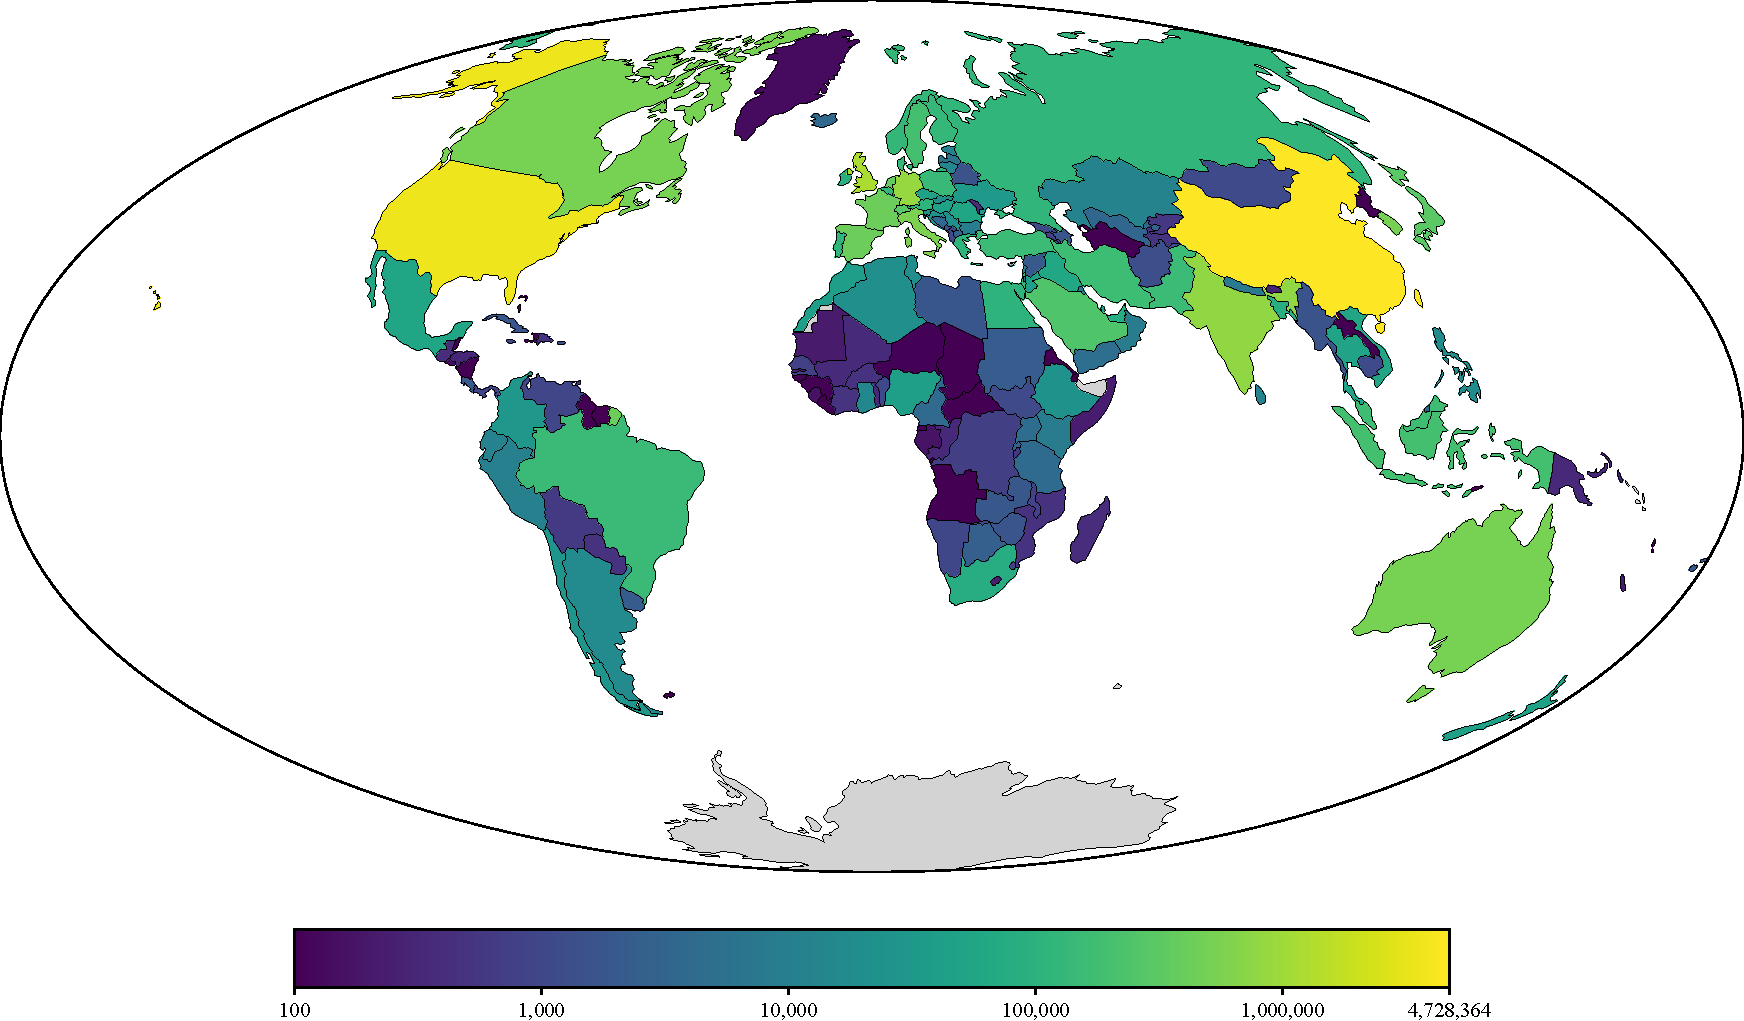
\includegraphics[width=\linewidth]{country_contributions_aitoff_log.pdf}
			\vspace{1em}
			\caption*{\small\textit{Figure 9 shows a Aitoff projection of the world map displaying the logarithmic distribution of national fractional citation sums. The lower bound is arbitrarily chosen to be at 100 while the upper bound is the maximum national value derived from the dataset.}}
			\label{logarithmic_distribution_citation_sum}
			\vspace{2em}
		\end{center}
	}]
	
	\paragraph{Fractional Citation Sums:} The citation sums are distributed so unevenly globally that a representation with a linear color-scale would assign only two countries with a color that can be easily distinguished from the minimum of the scale. These two countries are China with 4,728,364 citations and the USA with 3,648,720. Far behind them are the UK (1,220,273), Germany (876,943), and India (787,853). The Europeans can only compete with the national heavyweights as a collective: The EU-27 records a total of 4,079,623 citations. Among the IGOs, ASEAN (711,580) ranks next, ahead of Italy (568,825), Canada (525,273), and Australia (518,995). The African Union (402,405) would rank 12th if it was included in the country toplist. This is mainly due to the high citation totals for Egypt (106,599), South Africa (82,300), Nigeria (41,699), and Morocco (40,027). Surprisingly high values are also found in large parts of Asia. ASEAN member states Indonesia (190,576) and Malaysia (168,041) perform strongly, as do Saudi Arabia (242,000), Iran (160,776), and Pakistan (153,572). Mercosur (170,813), on the other hand, disappoints - it would rank 20th in the country ranking, just behind the city-state of Singapore (211,394). However, it should be remembered here that Spanish and Portuguese-language papers were among those most likely to be excluded by both the exclusivity of English search terms and again in the filtering of publications with non-English abstracts in the \nameref{quality_control_and_postprocessing}. In the case of Brazil, it can be assumed that a large proportion of the 13,721 Portuguese publications rejected were at the expense of the South American regional power. Given a publication volume of 42,121 after this sorting, a significant improvement in favor of Brazil but not entirely contradictory result can be expected. Japan's performance is equally underwhelming at 295,879 - the fourth-largest economy in terms of nominal GDP, ranks 13th in terms of citation sum, even behind its ambitious but considerably smaller neighbor South Korea (492,338).
	
	\paragraph{Citation Inequality:} To quantify inequality, one has to pick an \textit{ideal distribution} to calculate the observed distribution against. In the following, population sizes were chosen as parameters of that hypothetical equality. That means that AI-citations would be considered equally distributed, if countries' AI citation shares matched their population shares. The population-weighted Gini coefficient for total fractional citations sums amounts to 0.665. To put this into perspective: That means that AI-Research is not only distributed more unequal than the PPP-GDP (0.450), but even exceeds the more top-heavy nominal GDP distribution (0.632). This comparison demonstrates that the global geography of AI knowledge production is best described as an unequal and hierarchical system, in which scientific influence is concentrated in a small number of countries to an even greater extent than global value creation overall.
	
	\paragraph{Citation Overperformance:} When comparing the relative national shares of AI citations to each country’s share of global PPP-GDP, an interesting feature that could be called \textit{citation overperformance} is created. The resulting ranking shows that most overperforming outliers are found in Europe, where small yet innovation-driven economies exceed their expected citation volume by large margins: Finland produces 3.70 times its global economic share, followed by Switzerland (3.47), the UK (2.86), Denmark (2.61), Sweden (2.48), and the Netherlands (2.42). Beyond Europe, strong overperformers include Australia (2.72),  Israel (2.44), Singapore (2.37), and Canada (2.03). In contrast, the other blocs, the USA (1.26) and China (1.15), perform roughly on par with their global economic weight. On the lower end of the ranking, countries such as India (0.51), Japan (0.46), and Indonesia (0.41) contribute only about half as much to global AI research as their PPP-adjusted economic share would suggest. Mexico (0.18), Russia (0.16), and Argentina (0.12) are the weakest performers among the major economies in this metric.
	
	When instead using nominal GDP as the baseline, the picture shifts notably. Here, several OECD countries lose ground, while emerging markets become more prominent in comparison to their much smaller shares in the nominal GDP. Iran now leads the ranking, producing 2.7 times more AI citations than its nominal GDP share, followed by Pakistan (2.15) and Malaysia (2.15). Also noteworthy are Tunisia (1.91) and Egypt (1.76), whose relative citation output reveals growing ambitions in the field. In this perspective, China (1.33) significantly surpasses its economic share, while the USA (0.69) falls below it. India (1.19) and Indonesia (0.78) now perform roughly in line with their nominal GDP. Japan (0.41), Russia (0.32), and Mexico (0.20) remain the lowest-performing major economies as well in this metric. 
	
	
	
	
	\subsubsection{Multidimensional Performance Heatmap}
	\label{performance_heatmap}
	Building on the preceding world map, the analysis now refines this perspective by comparing national and regional research performance across twelve unique dimensions. \figurename~\ref{fig:research_performance_heatmap} displays those indicators for the 20 most-publishing countries and for the eight IGOs. The first five columns (Publication Share, Citation Share, Top-10\% Share, Top-1\% Share and Top-0.1\% Share) report each country’s share of the \textbf{Global AI Research Corpus}, while the subsequent rate-based indicators (Average Citations, Zero-Cited Rate, Within-Country Citation Inequality, Growth Rate, International Collaboration Rate, Field-Weighted Citation Impact, and Open-Access Rate) display the per-paper properties within each \textbf{National Subset}. To differentiate those two metrics the heatmap is split horizontally. Then it is split a second time vertically to preserve comparability across different groups of entities: The upper part ranks countries and the lower part ranks IGOs. The Viridis color-scale is normalized separately for each column and independently for countries and IGOs, ensuring that aggregated volumes of big entities like the Global South do not compress all values countries into the lower end of the shared color-scale. In the following, each of the twelve columns is examined in sequence to provide an explorative reading of the underlying patterns, without claiming interpretative exhaustiveness.
	
	\paragraph{Publication Share:} The heatmap confirms the head-heavyness of the distribution of publications. Four countries cover more than half of publications (51.5\%). 25.2\% of all AI publications are published by authors from Chinese institutions, followed by the US with 15.2\%, India with 6.7\% and the UK with 4.4\%. Taken as a bloc the EU-27 contributes 18.5\% and would thus rank even higher than the US. Interestingly, the OECD and G-77 are very close with 50.2\% and 47.3\% respectively. The difference between the G-77, which records 134 members and BRICS+, which has 10 memebers in June of 2025 reveals that 124 countries of the Global South contribute less than 10\% of AI publications.
	
	\paragraph{Citation Share:} The citation aggregates are even more concentrated among the top four countries, which cover 53.4\% of the global sum. India (4.02\%) slips to fifth rank, overtaken by the UK (6.22\%) and Germany (4.47\%). The share of the OECD thereby grows to 58.8\% while the G-77 shrinks to 39.9\%. Similar to the results of the comparison between citation sums and GDP, which was performed for the \textit{citation-overperformance} in the \nameref{citation_geomapping}, the biggest profiteers when comparing citation shares against publication share are high income countries. Especially great is the leap for anglophone countries - with Australia contributing 1.51 times more in citation share than in publications share. The UK follows with 1.42, the USA with 1.22 and Canada with 1.20 - all well above  the EU-27’s 1.13. China on the other hand slightly underperforms with 0.95.
	
	\twocolumn[{%
		\begin{center}
			\vspace{-3em}
			\refstepcounter{figure}
			\captionof{figure}{Multi-Dimensional Research-Performance Heatmap}
			\vspace{2em}
			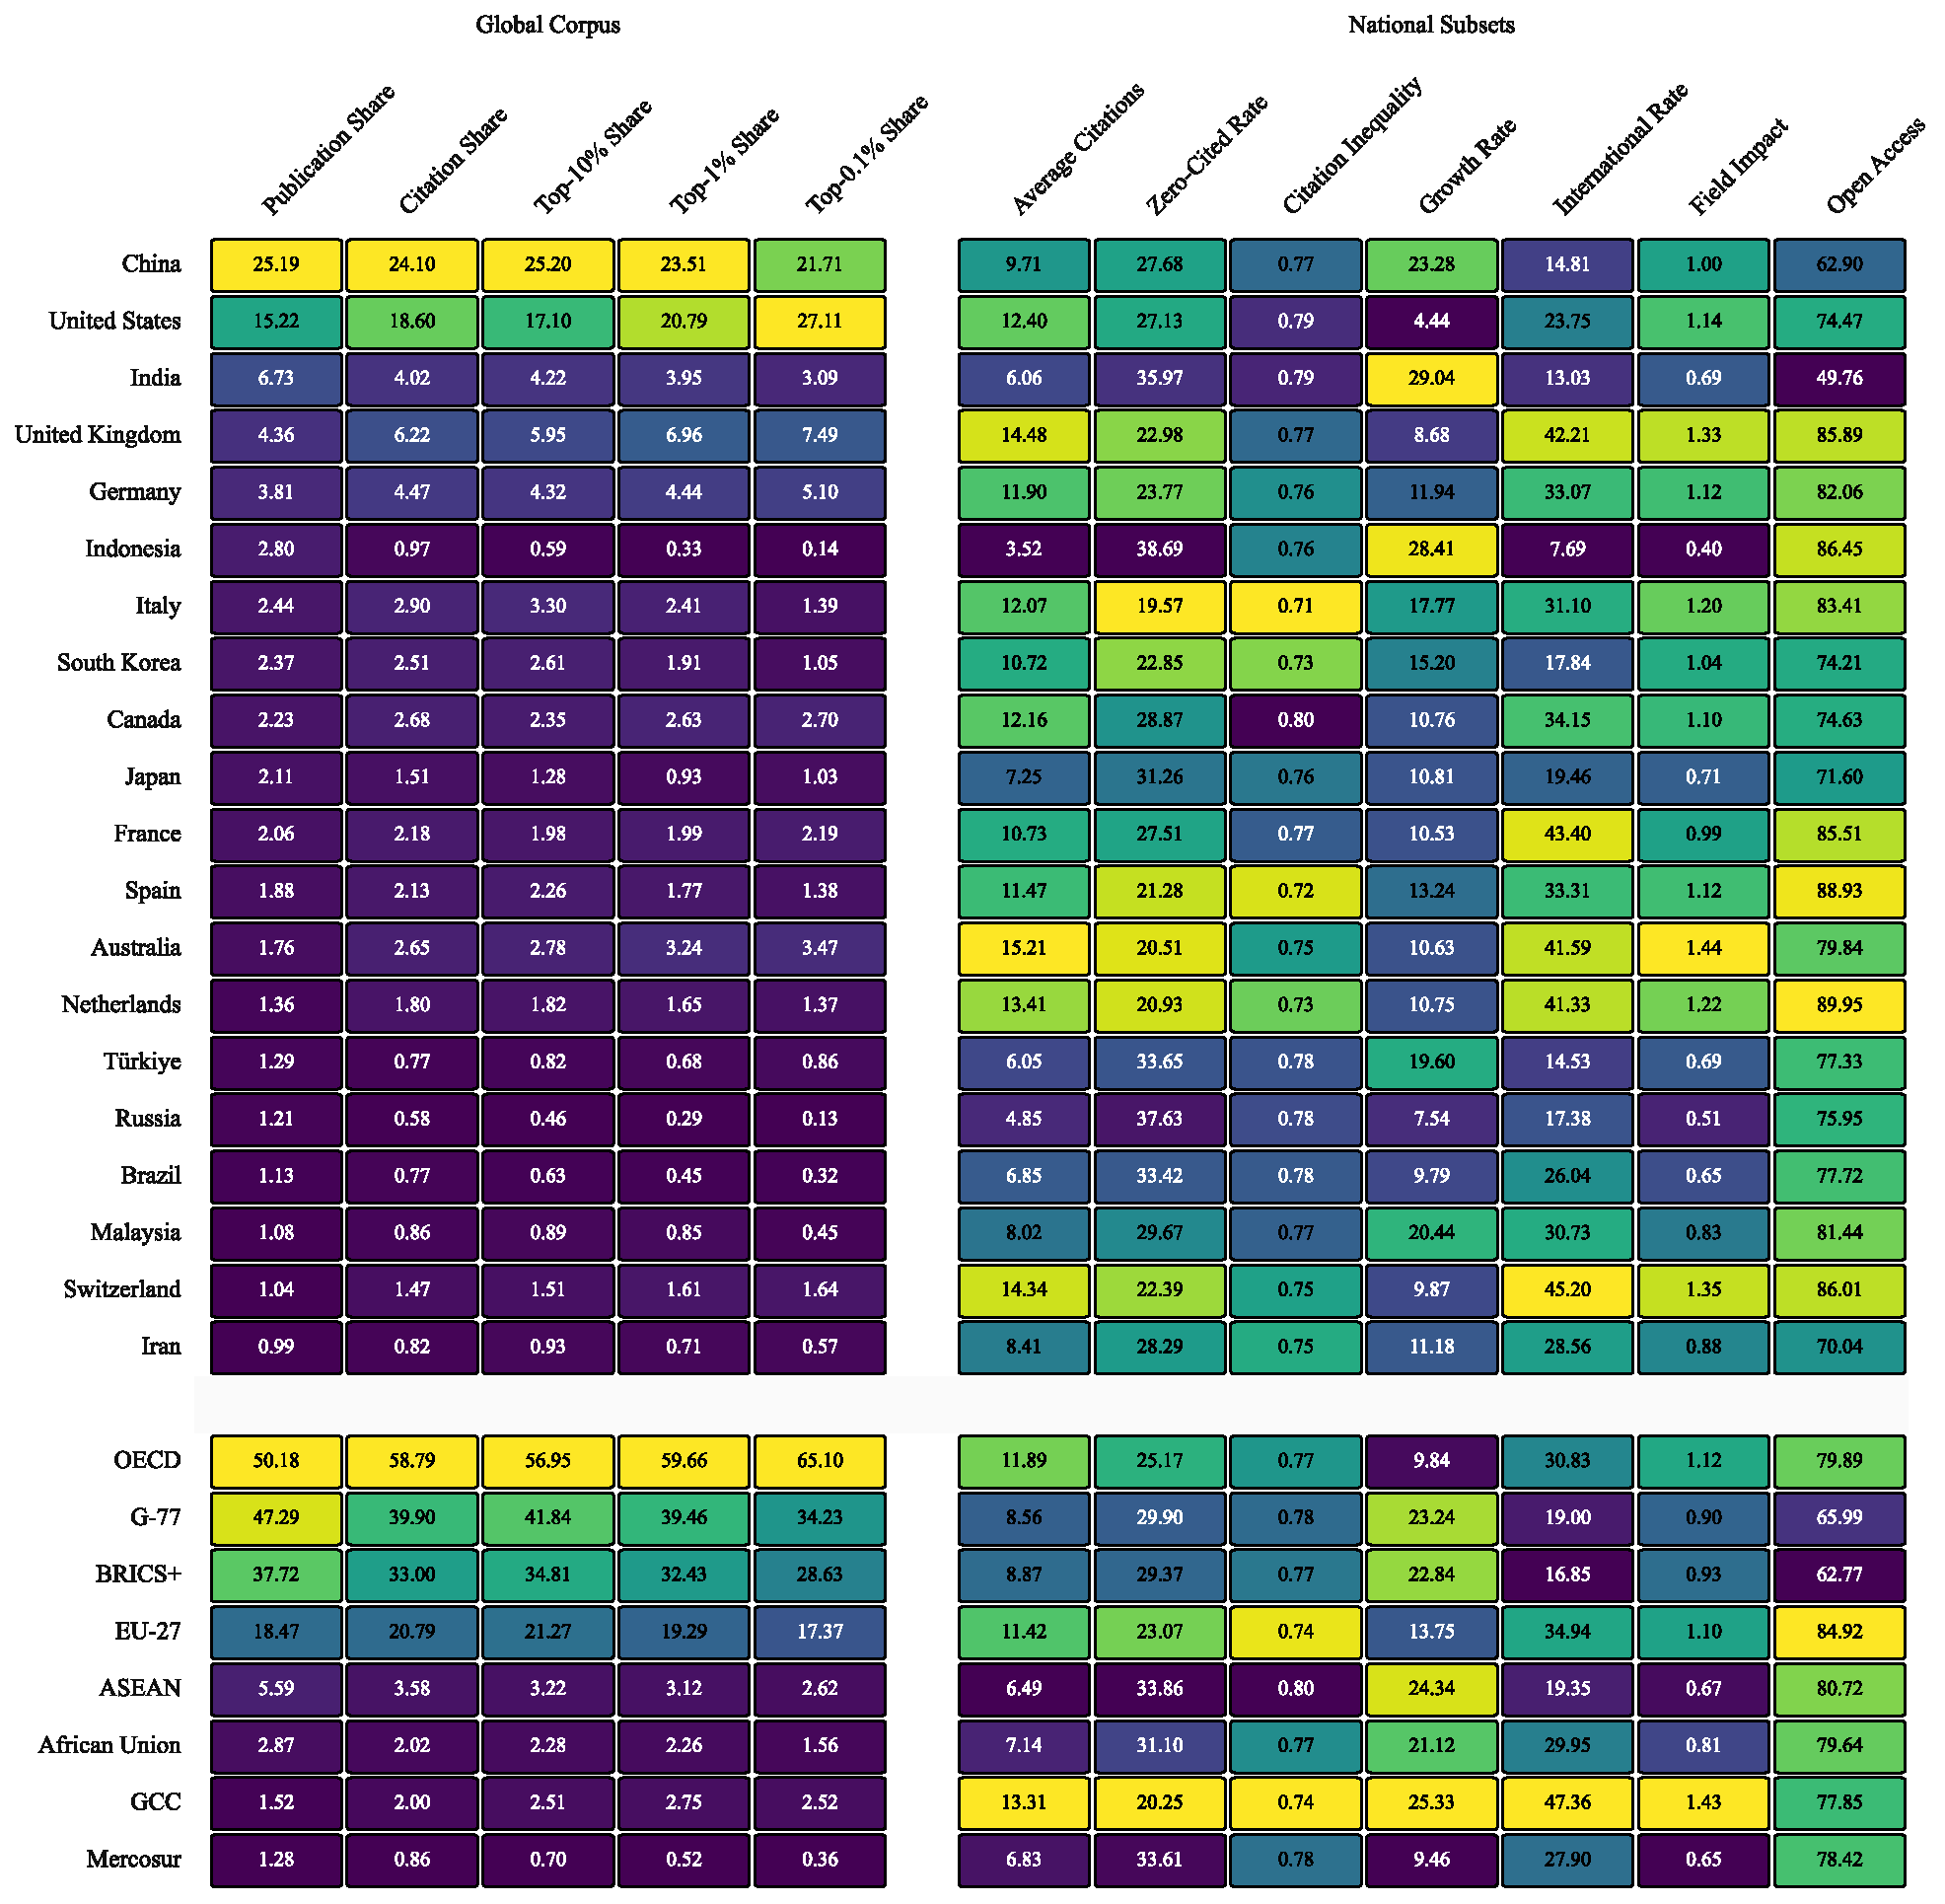
\includegraphics[width=\linewidth]{new_heatmap.pdf}
			\vspace{1em}
			\caption*{\small\textit{Figure 11 shows a heatmap of twelve research performance indicators. The color-scaling within the heatmap is done a total of 24 times - for each of the twelve indicator its done first for the countries on top and then for the IGOs on the bottom. The five columns on the left side present entity's share of the global dataset. The seven columns on the right represent entity's performance per paper. Normalization is rigidly done by setting the color-scale bounds to the minimum and maximum of the currently observed set of entities.}}
			\label{fig:research_performance_heatmap}
			\vspace{2em}
		\end{center}
	}]
	
	\paragraph{Shares of Most-Cited Publications:} The next three columns show country's shares of the most-cited publications. They suggest an intensification of research performance concentration the higher the percentile gets. India, Indonesia and all other non-OECD countries except for the GCC members show consistent decline from their publication share to their share of the top 0.1 percentile. This phenomenon can best be described when looking at the Top-1\% Shares column: Here Indonesia underperforms its publication share by a factor of 20, Russia by 9.3, Brazil by 3.53 and India by 2.18. Meanwhile the four western anglophones - US (1.37), UK (1.60), Canada (1.18), and Australia (1.84) - as well as Germany (1.17) and Switzerland (1.55) are the biggest profiteers when compared to their publication share. While the US is still behind China in top-10\% and top-1\% papers it overtakes their 21.71\% with 27.1\% of the 1987 most-cited papers. OECD countries cover 65.1\% of top-0.1\% papers and the G-77 34.2\%. Interestingly, there are significant differences within the OECD members. While the US-share grows 10.01\% from top-10\% share to top-0.1\% share that of the EU27 drops by 3.90\%, indicating the EU-27s broad and comprehensive representation among papers of the first and second quarter, while falling a little behind in terms of the most-cited elite-publications. Another high-performing IGO that has received little attention up to now is the GCC which is home to 2.75\% of the most-cited percentile. With that share it is outcompeting well established AI actors like Canada and is - at least in this elitist indicator - close to all of India.
	
	\paragraph{Average Citations:} The average citations is the first column that does not show national percentages of the global dataset, but compares national subsets of the corpus on a per-paper basis. This switch of mode results in a ranking vastly different from that based on the publication share. The range of national averages are considerable, with Indonesia showing the minimum of the 20 countries at 3.5 citations per work while Australia leads with 15.2. EU-27 countries fluctuate around the average of 11.42, while the US reports 12.4 and China 9.7. China's average is significantly lower than that of the OECD (11.9), yet significantly higher than the G-77 (8.56). Again the weakest performances among the observed entities are found in Indonesia (3.52), Russia (4.85), Türkiye (6.05) and India (6.06).
	
	\paragraph{Zero-Cited Rate:} After the location of the most successful papers, the focus now shifts to the least successful: Those which were never cited. One must note that the numbers are a snapshot of the downloading date in July 2025. That means that the most recent papers of the dataset were published for only six months and therefore had very little time to accumulate citations. High rates of zero-cited publications can therefore partly be explained by high growth rates which indicate overproportionality of newer papers over older ones. Yet results are largely consistent with the average citations contributing to the assumption of rather continuous national distribution. Indonesia (38.7), Russia (37.6), and India (36.0) again stand out with large percentages whereas EU-27 countries (23.1), South Korea (22.9) and Australia (20.5) show the lowest numbers. China (27.7) and the US (27.1) both score mediocre in this performance metric and therefore the difference between OECD (25.2) and G-77 (29.9) is smaller than in most previous metrics.
	
	\paragraph{Citation Inequality:} Now that the shares of most and least successful papers were quantified an analysis of their distribution within the national sub-corpora is done to measure the degree of citation distribution inequality using the Gini coefficient. For its calculation, citation sums were normalized against their publication year. Note that the missing granularity of the publication date favors works published earlier in the year. The metric shows that all countries have very high citation inequality of Gini coefficients higher than 0.7 and averaging at 0.76. There is little regional or organizational consistency with the EU-27 scoring best with 0.74 and ASEAN worst with 0.80. China and the US score similarly high with 0.77 and 0.79 respectively. Canada shows the most unequal citation distribution among the 20 most-publishing countries with 0.80. Taken together the Gini coefficient shows that the winner-takes all principle is applicable to academia across the world. As described in the Matthew effect, often-cited papers are more visible, more trusted and therefore chosen more often as reference, creating a feedback loop inflating citation counts of publications that (i) are published early (2) originate from legacy institutions, (3) have access to institutional infrastructure of academia \cite{Merton1968}.
	
	\paragraph{Growth Rate:} To establish which countries are making the fastest progress in AI research, the growth rate is calculated as CAGR of publication volume from 2020 to 2023. The CAGR of AI-related publication are positive for all 28 entities. The five countries with the highest rates are all located in Asia with India (29.04\%) and Indonesia (28.41\%) leading the ranking. China is third with 23.3\% while the US has the lowest rate among the observed countries with 4.4\%. However, this metric should be interpreted with caution for two reasons. First, it does not reveal what share of each country’s overall research output is related to AI. The US, for example, may already have reached a level of saturation in AI research by 2020, while several Asian countries are still in a phase of catching up to the global research front. Second, the metric does not distinguish whether AI growth reflects a growth in the share of AI-related research measured against overall research or merely mirrors a broader increase in total research production. What is clear, however, is that publication growth in the G-77 substantially outpaced that of the OECD countries with 23.2\% and 9.8\% retrospectively suggesting a notable shift in global AI research dynamics if the trajectory persists.
	
	\paragraph{International Cooperation Rate:} International cooperation between academic institutions is not only considered a marker of research quality and credibility but has proven to increase research quality by pooling resources, diversifying methodologies and exploiting network effects \cite{kohus2022influence}. The observed dataset gives further evidence to this hypothesis. The suggested correlation between average citations and international cooperation is strikingly strong with a Spearman's $\rho$ of 0.81 when comparing the rankings of the 20 countries. However, the numbers cant tell the directions of causality apart - publications could harvest success for their internationality or get internationalized by their (anticipated) success. The calculation of the share of international cooperation was based on the following definition: A work is considered \textit{international} when not all institutions of the publishing authors are located in the same country. Yet it must be considered that geographic and cultural proximity are not always best described by nation borders. A cooperation between the \textit{Indian Institute of Technology Madras} in Chennai and the \textit{University of Chandigarh} might satisfy the premises of the underlying hypothesis even more than a cooperation between the \textit{Technical Universities of Munich} and the \textit{University of Innsbruck} even though only the latter is considered to be international cooperation. Looking at the numbers, we can see that the rates differ significantly across the globe, ranging from Indonesia's 7.7\% to Switzerland's 45.2\%. The EU members fluctuate around the average of 34.9\% with many of the highest values in the ranking. Larger countries show the expected tendency toward internal saturation of cooperation networks. They record significantly lower rates: The US sits at 23.8\%, China at 14.8\% and India at 13.0\%, way below the G-77 rate of 19.0\%. The highest score among the 28 entities is once again to be found at the GCC which see international cooperation at nearly half of their publication. 
	
	\paragraph{Field Weighted Citation Impact:} To normalize against differences in national subdiscipline distribution the FWCI was calculated. The results show clear disparities between established and emerging research systems. The US (1.14), the EU-27 (1.10), and the OECD as a whole (1.12) maintain citation levels well above the global mean, reflecting broad and sustained influence across fields. Australia (1.44), the GCC (1.43), and Switzerland (1.35) outperform these large entities, indicating exceptionally high visibility per paper. China, by contrast, aligns exactly with the global average (1.00), while Japan (0.71), India (0.69), Russia (0.51), and Indonesia (0.40) fall significantly below that. This pattern mirrors a wider divide between the OECD (1.12) and the G-77 (0.90), suggesting that while emerging economies are rapidly expanding their publication volume, their citation visibility still lags behind that of established research hubs.
	
	\paragraph{Open-Access Rate:}
	The final metric in the provided research performance heatmap measures the share of publications that are freely accessible to the global research community. In scientometrics open-access is widely recognized as a key factor that accelerates the dissemination of knowledge and enhances its societal reach, making research outcomes more transparent and widely usable \cite{Piwowar2018}. Across countries, open-access rates vary considerably - from India’s 49.8\% at the lower end to the Netherlands’ remarkable 90.0\%. Within the blocs, the EU-27 reaches an average of 84.9\%, followed by the US with 74.5\% and China with 62.9\%. A similar pattern appears at the regional level, where the OECD averages at 79.9\% and the G-77 at 66.0\%. The latter figure, however, is largely driven by the relatively low values of China and India. Several other G-77 members, such as Indonesia (86.5\%), Malaysia (81.4\%), Brazil (77.7\%), and Russia (76.0\%), achieve open-access levels comparable to those of the EU-27. At the same time the open-access rates of OECD members like Canada (74.6\%), South Korea (74.2\%), and Japan (71.6\%) suggest that accessibility in AI research is neither uncommon in the Global South nor guaranteed in the Global North.
	
	\subsubsection{National Citation Percentile Distribution}
	\label{citation_percentile_distribution}
	In the \nameref{performance_heatmap}, countries and regions were already compared by their share of the world’s most and least cited AI publications. The next step completes this layer of analysis by mapping the distribution of citation percentiles within each national subset. For that purpose, the fractional citation sums are again normalized against their publication years to remove age effects and enable cross-national comparability. \figurename~\ref{fig:citation_percentile_distribution} presents within-country profiles for the 20 most-publishing nations. Each horizontal bar equals 100\% of a country’s or IGO's output and is partitioned into citation percentile bands (0-25, 25-50, 50-75, 75-90, 90-99, 99-100). Right-heavy bars signal a larger share of papers in the upper percentiles and thus reflect disproportionate high-impact contributions, whereas left-heavy bars indicate concentration in lower-impact segments. The percentile distribution plot offers a compact view of research quality across all citation percentiles.
	
	However, the interpretation of the percentile distribution is compromised by two structural weaknesses: (i) \textbf{Zero-Cited Inflation:} The band of the lowest 25\% is inflated in size, because zeros remain zeros even after year-normalization. Since more than 25\% of the global dataset consists of zero-cited papers, it logically follows that the papers falling into the lowest quartile of the citation distribution must also account for more than 25\%. (ii) \textbf{Incomplete Accumulation:} Citation accumulation and the Matthew-Effect require time. Working with a contemporary dataset, the \textit{winner-takes-all} dynamic has not yet fully emerged. This temporal constraint compresses the distribution’s upper extremes. Consequently this analysis should be understood as an intermediate snapshot that is structurally biased toward the center, with exceptional outliers not yet fully developed. Despite these caveats, substantive cross-national differences were found and are presented in the following.
	
	China and the US, the two dominant national producers of AI-related research, are strikingly similar across the lower and middle percentile bands. Only at the very top the US displays a modest advantage: Its shares in the 90-99\% and 99-100\% citation strata are larger, reflecting a slightly stronger concentration of globally leading publications. The percentile distribution of the EU-27 diverges from that pattern. 
	
	\twocolumn[{%
		\begin{center}
			\vspace{-3em}
			\refstepcounter{figure}
			\captionof{figure}{National Year-Normalized Citation Percentile Distribution}
			\label{fig:citation_percentile_distribution}
			\vspace{1em}
			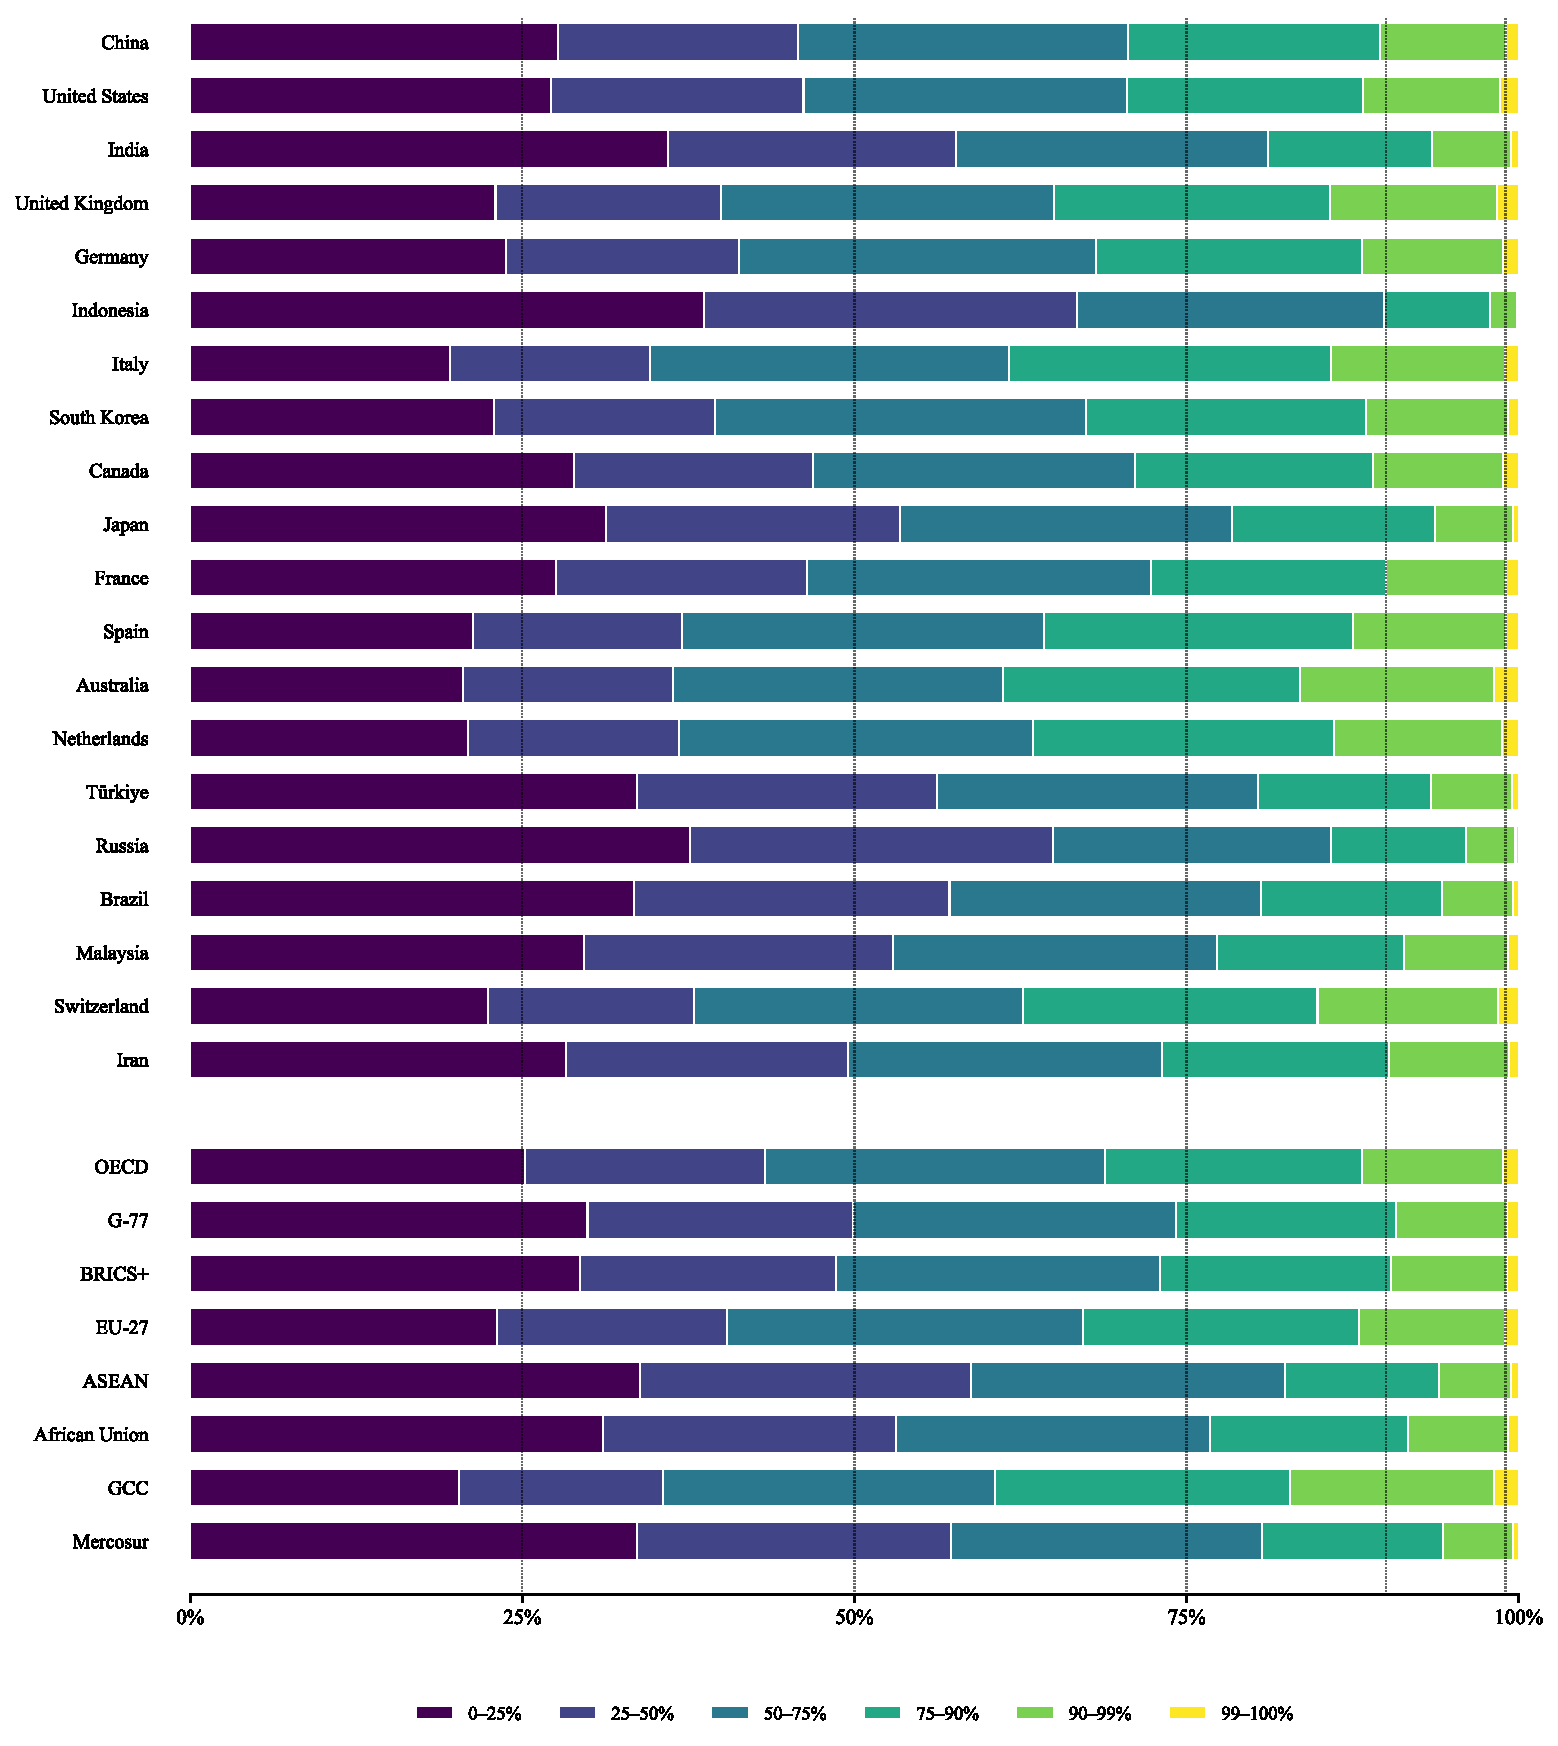
\includegraphics[width=\linewidth]{percentile_composition_top20_countries_plus_blocs.pdf}
			\vspace{1em}
			\caption*{\small\textit{Figure 13 shows the distribution of the fractional citations percentiles within the national subsets of the 20 most-publishing countries and eight IGOs. Each horizontal bar represents an entity’s publication output normalized to 100\%, partitioned into six year-adjusted citation bands (0-25\%, 25-50\%, 50-75\%, 75-90\%, 90-99\%, 99-100\%). The inflated size of the lowest quartile reflects the fact that the global share of zero-cited papers frequently exceeds 25\%, thereby artificially compressing the intermediate bands.}}
		\end{center}
	}]
	
	It undercuts the 25\% mark with its least cited quarter and instead sees bigger shares in the third quartile publications and the band from 75\% to 90\%. Even in the top 10\% publications the EU-27 outperforms both China and the US with 12.7\% of their papers among that elite group. However, in the top-1\% band the EU-27 falls behind and, reching a level in between China (0.98\%) and the US (1.28\%) with 1.15\%.
	
	Smaller but research-intensive countries such as Australia, the UK, and Switzerland perform strongly in terms of their citation percentile distribution: They produce a disproportionately high share of papers in the top quartile and especially in the top decile, underscoring how well-resourced and internationally connected middle-sized systems can leverage quality in spite of smaller output volume. In stark contrast, emerging systems such as India, Indonesia, Russia and Brazil lag behind substantively. In the case of Indonesia, less than ten percent of their publications reach the global top quartile, and only 0.11\% reach the top percentile. Yet there are outliers beyond China in the Global South: Malaysia and Iran score largely on par with the global dataset. And outliers also exist among the OECD countries: Again Japan underwhelms in higher citation strata with 6.4\% in the top decile and 0.46\% in the top percentile. Yet those are outliers that are contradicting a global trend which still shows that the rapid expansion of publication quantities among countries of the Global South has apart from China and the GCC largely not yet caught up qualitatively. The OECD as a collective still outperforms the G-77 in terms of high-percentile shares, but the gap is narrower than might be expected given historical patterns, indicating the increasing presence of high-quality research in the Global South, especially but not exclusively due to China's scientific expansion. 
	
	\subsubsection{Institutional Co-Authorship Network}
	\label{institution_network}
	The perspective of the distribution of citation percentiles at the national level, however, leaves several questions unanswered. For example, it remains unclear where the EU-27's buldged middle - the strong concentration of publications between the 50th and 99th percentiles - comes from and why both the US and China show a distribution that is more concentrated towards the edges. Another interesting question would be how concentrated research output is within small high-performing countries such as Switzerland, Australia, or the Netherlands. In order to answer these questions, the perspective of countries as monolithic blocks will be abandoned in favor of a view at the institutional level. Specifically, a network graph of the 1000 institutions with the biggest sums of fractional citations is constructed. Each institution is assigned to one of the three blocs with a fourth residual label for RoW. The resulting network is laid out using the ForceAtlas2 algorithm, with node sizes proportional to an institution’s cumulative fractional citation sums and edge weights reflecting the intensity of inter-institutional co-authorship \cite{jacomy2014forceatlas2}. While all edges were included for the simulation of the presented graph layout, only edges with a weight greater than or equal to 1.0 are displayed to reduce visual clutter. The threshold of 1.0 would for instance be satisfied if two publications of balanced cooperation between two institutions were found in the dataset.
	
	
	
	
	While a variety of graph-theoretical centrality metrics could, in principle, be applied to this network, their interpretive validity is limited in the present context. The following discussion outlines why measures such as \textit{PageRank} and \textit{Eigenvector Centrality} are not suitable for capturing meaningful institutional research impact in this dataset despite their overall popularity in scientometrics.
	
	\paragraph{PageRank:} When the PageRank is applied to the institutional co-authorship network, China is found to be the in the lead, with 31 of the 100 highest-ranked institutions, compared to 28 from the EU-27, 20 from the US and 21 from RoW. The \textit{Chinese Academy of Sciences} occupies the first position with a PageRank score of 0.0197, more than twice that of its nearest competitor. This outcome stems not from superior research quality, but from structural properties that the PageRank algorithm inherently favors: China’s top-heavy university system, the high internal density of its co-authorship network, and its low external linkage to non-Chinese institutions. The PageRank thus systematically rewards exactly those characteristics that are widely regarded as systemic weaknesses of a research ecosystem. For that reason, PageRank is considered inapplicable to a longitudinal cross-country comparison, facing different scientific systems and cultures.
	
	\paragraph{Eigenvector Centrality:} The eigenvector centrality performs equally poorly under these structural conditions. On dense and undirected networks such as institutional co-authorship graphs, the leading eigenvector tends to approximate degree centrality, effectively mirroring the number of connections rather than their strategic importance. This produces a flattened node-size distribution and eliminates meaningful differentiation between core and peripheral institutions. Moreover, umbrella organizations like the \textit{Centre National de la Recherche Scientifique} appear disproportionately central due to their wide co-affiliation footprint and despite their relatively poor fractional citation sums. The divergence of those two results stems from an overproportional participation in publications that record contributions from many other institutions.
	
	Given these methodological constraints, fractional citation totals remain the most transparent and robust indicator of institutional centrality. Citations offer a direct, interpretable, and empirically grounded measure of research impact that is already subject to a mature body of critique capable of contextualizing their interpretative boundaries (for more, see \nameref{conclusion_limitations}). In the following, attention is first turned to the distribution of nodes across the three blocs and RoW. Then, the focus is shifted to the topology of the presented network. Here, the spotlight is on neighborhood relationships, cluster densities, and node sizes. Finally, the 100 most-cited institutions, which can also be found in the table below \figurename~\ref{fig:cn_eu_us_top_1000_institutions}, are examined in terms of position, origin, and institutional type.
	
	\twocolumn[{%
		\begin{center}
			\vspace{-3em}
			\captionof{figure}{Co-Authorship Network of the 1000 Most-Cited Institutions}
			\vspace{1em}
			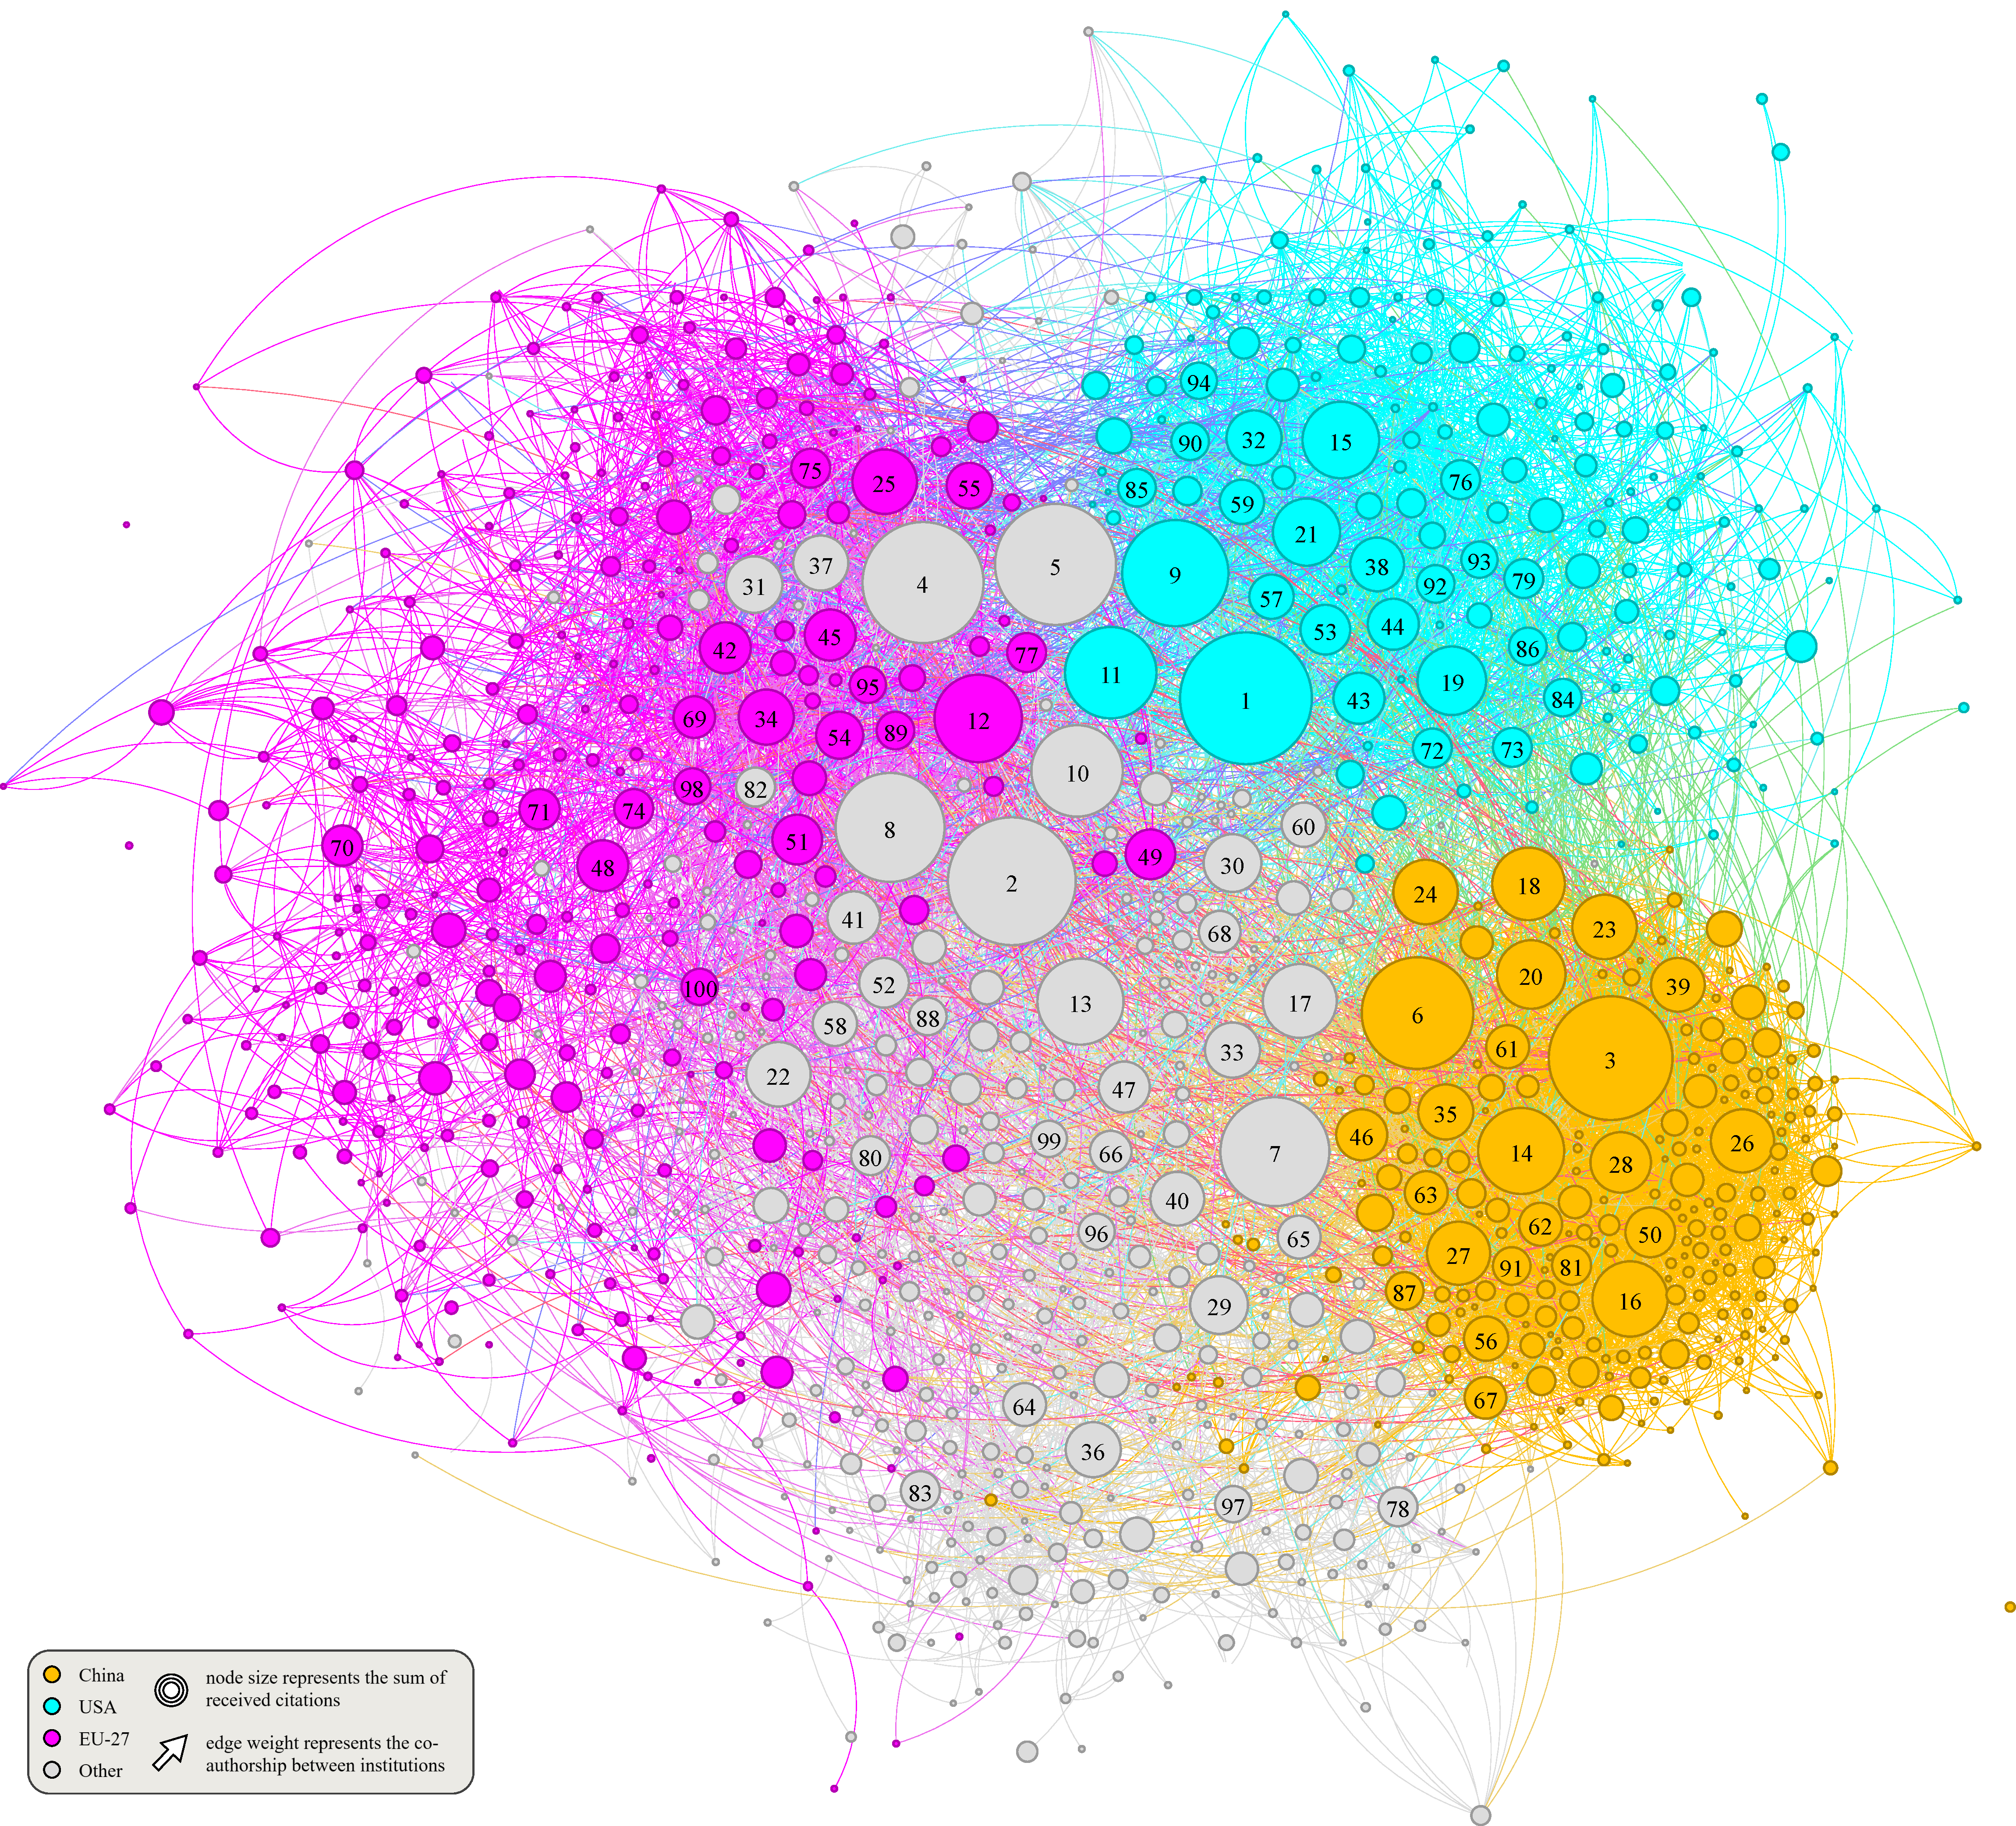
\includegraphics[width=0.9\linewidth]{institution_network_top_1000_with_legend.pdf}
			\label{fig:cn_eu_us_top_1000_institutions}
			\vspace{1em}
			
			\tiny
			\setlength{\tabcolsep}{6pt}
			\renewcommand{\arraystretch}{1.12}
			\begin{tabular}{@{}l l l l l l@{}}
				\toprule
				\addlinespace[1.0em]
				\rc{1}{US}  & Stanford University &
				\rc{35}{CN} & Tongji University &
				\rc{69}{FR} & Centre National de la Recherche Scientifique \\
				\rc{2}{GB}  & University of Oxford &
				\rc{36}{SA} & King Abdulaziz University &
				\rc{70}{IT} & Sapienza University of Rome \\
				\rc{3}{CN}  & Chinese Academy of Sciences &
				\rc{37}{CH} & University of Zurich &
				\rc{71}{IT} & University of Padua \\
				\rc{4}{CH}  & ETH Zurich &
				\rc{38}{US} & University of Pennsylvania &
				\rc{72}{US} & Pennsylvania State University \\
				\rc{5}{GB}  & DeepMind &
				\rc{39}{CN} & University of Chinese Academy of Sciences &
				\rc{73}{US} & University of Illinois Urbana-Champaign \\
				\rc{6}{CN}  & Tsinghua University &
				\rc{40}{AU} & UNSW Sydney &
				\rc{74}{IT} & University of Bologna \\
				\rc{7}{AU}  & Monash University &
				\rc{41}{GB} & King's College London &
				\rc{75}{DE} & Ludwig\mbox{-}Maximilians\mbox{-}Universität München \\
				\rc{8}{GB}  & University College London &
				\rc{42}{NL} & Utrecht University &
				\rc{76}{US} & University of Wisconsin-Madison \\
				\rc{9}{US}  & Harvard University &
				\rc{43}{US} & University of California, San Diego &
				\rc{77}{DK} & University of Copenhagen \\
				\rc{10}{GB} & University of Cambridge &
				\rc{44}{US} & University of California, Los Angeles &
				\rc{78}{KR} & Seoul National University \\
				\rc{11}{US} & Massachusetts Institute of Technology &
				\rc{45}{NL} & Wageningen University \& Research &
				\rc{79}{US} & University of Florida \\
				\rc{12}{NL} & Delft University of Technology &
				\rc{46}{HK} & Hong Kong Polytechnic University &
				\rc{80}{GB} & University of Manchester \\
				\rc{13}{GB} & Imperial College London &
				\rc{47}{AU} & The University of Melbourne &
				\rc{81}{CN} & Chongqing University \\
				\rc{14}{CN} & Zhejiang University &
				\rc{48}{IT} & Politecnico di Milano &
				\rc{82}{NO} & University of Oslo \\
				\rc{15}{US} & University of Washington &
				\rc{49}{DK} & Technical University of Denmark &
				\rc{83}{IN} & Vellore Institute of Technology \\
				\rc{16}{CN} & Central South University &
				\rc{50}{CN} & Sichuan University &
				\rc{84}{US} & Georgia Institute of Technology \\
				\rc{17}{SG} & National University of Singapore &
				\rc{51}{NL} & University of Twente &
				\rc{85}{US} & Broad Institute \\
				\rc{18}{CN} & Wuhan University &
				\rc{52}{GB} & University of Edinburgh &
				\rc{86}{US} & University of California, Davis \\
				\rc{19}{US} & University of Michigan &
				\rc{53}{US} & Johns Hopkins University &
				\rc{87}{CN} & Xi'an Jiaotong University \\
				\rc{20}{CN} & Shanghai Jiao Tong University &
				\rc{54}{NL} & University of Groningen &
				\rc{88}{GB} & University of Glasgow \\
				\rc{21}{US} & University of California, Berkeley &
				\rc{55}{NL} & University of Amsterdam &
				\rc{89}{DK} & Aarhus University \\
				\rc{22}{NO} & Norwegian University of Science and Technology &
				\rc{56}{CN} & Harbin Institute of Technology &
				\rc{90}{US} & Columbia University \\
				\rc{23}{CN} & Peking University &
				\rc{57}{US} & Yale University &
				\rc{91}{CN} & Beijing Institute of Technology \\
				\rc{24}{HK} & University of Hong Kong &
				\rc{58}{GB} & University of Bristol &
				\rc{92}{US} & Carnegie Mellon University \\
				\rc{25}{DE} & Technical University of Munich &
				\rc{59}{US} & New York University &
				\rc{93}{US} & University of Southern California \\
				\rc{26}{CN} & Huazhong University of Science and Technology &
				\rc{60}{CA} & University of British Columbia &
				\rc{94}{US} & Cornell University \\
				\rc{27}{CN} & University of Electronic Science and Technology of China &
				\rc{61}{CN} & Fudan University &
				\rc{95}{NL} & Radboud University Nijmegen \\
				\rc{28}{CN} & Sun Yat-sen University &
				\rc{62}{CN} & Beihang University &
				\rc{96}{AU} & Queensland University of Technology \\
				\rc{29}{QA} & Qatar University &
				\rc{63}{CN} & Southeast University &
				\rc{97}{KR} & Sejong University \\
				\rc{30}{CA} & University of Toronto &
				\rc{64}{SA} & King Saud University &
				\rc{98}{BE} & Ghent University \\
				\rc{31}{CH} & École Polytechnique Fédérale de Lausanne &
				\rc{65}{JP} & The University of Tokyo &
				\rc{99}{AU} & The University of Sydney \\
				\rc{32}{US} & University of California, San Francisco &
				\rc{66}{AU} & The University of Queensland &
				\rc{100}{FI} & University of Helsinki \\
				\rc{33}{SG} & Nanyang Technological University &
				\rc{67}{CN} & Northwestern Polytechnical University & & \\
				\rc{34}{BE} & KU Leuven &
				\rc{68}{CA} & University of Waterloo & & \\
				\addlinespace[2.0em]
			\end{tabular}
			\caption*{\small\textit{Figure 14 shows a co-authorship network of the 1000 most-cited institutions. The layout is generated with the ForceAtlas2 Algorithm. Each node represents one institution, each edge the degree of co-authorship between institutions. Institutions are attributed to the blocs and the residual RoW-cluster. The table shows the 100 most-cited institutions also labeled in the graph.}}
		\end{center}
	}]
	
	\paragraph{Node Distribution:} First, the origins of the 1000 most-cited institutions will be examined. The EU-27 contributes 282 nodes, China 213, the US 161, and the rest of the world 344 of the 1,000. That is in stark contrast to the distribution of fractional citations found earlier, where China accumulated the highest sum with 4.76 million citations, followed by the EU-27 with 4.11 million, the US with 3.67 million, and RoW with 7.28 million. This indicates that China's citation count is concentrated within a smaller set of elite institutions, whereas Europe’s influence is spread more evenly across a larger number of universities and research centers. The US likewise shows strong concentration, with comparatively few institutions capturing a disproportionately large share of citations. However, there are alternative explanations that have little to do with national research impact. for example, it is plausible that there are systematic differences in the size of research institutions and therefore that more fragmented research systems are wrongly penalized by the design of such rankings. In China such concentration of research resources has been actively promoted through the \textit{Project 211} and \textit{Project 985} as well as the creation of the \textit{C9 League}, which together channeled resources into a small circle of elitist universities. In the US, a similar elite stratum is represented by the \textit{Ivy League}. Europe, by contrast, lacks a directly comparable pan-European initiative, although national excellence initiatives have sought to consolidate and strengthen a subset of universities.
	
	\paragraph{Network Topology:} Now that the geographic composition of the nodes is established, the graph can be examined to analyze its topology. The graph’s layout is driven by three forces, (i) the node counts by bloc, (ii) the node sizes based on fractional citation sums, and (iii) the intensity of intra- and inter-cluster co-authorships. The EU-27 cluster is characterized by a comparatively large number of medium-sized nodes and extends across the entire western half of the graph, reflecting the heterogeneity and broad dispersion of research funding within the bloc. In the north, the European cluster borders and partially converges with its American counterpart. The latter has a similar local density but comprises 121 fewer nodes than the EU-27 and is therefore considerably smaller. Five of the ten most-cited institutions are from the RoW-cluster and act as a broker between the US and the EU-27. Four of them are from the UK (\textit{Oxford}, \textit{UCL}, \textit{Cambridge}, and \textit{Deepmind}) and one from Switzerland (\textit{ETH Zurich}). Likewise, the three most-cited institutions of the US (\textit{Standford}, \textit{Harvard}, \textit{MIT}) are strongly oriented towards the EU-27 cluster, reflecting intense transatlantic collaboration epsecially among the most-cited institutions. In the south western region of the graph China’s institutions form a more dense cluster, consistent with its relatively lower international cooperation rate and strong domestic integration. Despite its 213 nodes, the Chinese subgraph takes less space than its US-counterpart of only 161 nodes. 
	
	Interestingly, for China its not the most-cited institutions that are closest to the center edges but medium-sized nodes like \textit{Tsinghua University} and the \textit{Wuhan University} as well as the \textit{University of Hongkong} and \textit{Hong Kong Polytechnic University}. Meanwhile, China's fourth ranked \textit{Central South University} borders the peripheral rim of the cluster opposite the graphs center and thus furthest from the cross-country co-authorship corridor. Even China's most-cited institution, the \textit{Chinese Academy of Sciences} is embedded centrally within the domestic scientific system. Striking is also the fact that the Chinese cluster is closer to the US-cluster than to the EU-27-cluster. Or put differently: Between the EU-27 and China lies a corridor of nodes from the RoW-cluster that effectively insulates the two. That corridors national composition is further discussed in the following paragraph.
	
	\paragraph{The 100 Most-Cited Institutions:} To learn more about the institutional type and (sub-bloc) geographic properties of the nodes, the 100 most-cited institutions are identified and analyzed separately. The labeling reveals the composition of the institutional types: Of the 100 nodes, 96 represent universities. The remainder consists of three institutes focusing on management and funding of research (\textit{Chinese Academy of Sciences}, \textit{Centre National de la Recherche Scientifique}, and \textit{Broad Institute}) and only one private research laboratory (Google's \textit{Deepmind}, which is labeled after its British origin by OpenAlex). This pattern should not be read as evidence of private-sector weakness in AI R\&D, but rather as a limitation of scientometrics: Corporate research often remains underrepresented in scientific datasets relative to publicly funded academia for the obvious reason of shielding knowledge margin against competitors.
	
	More can also be learned about the national distribution within the EU-27, in which 20 of the 100 institutions are located (China 23, the US 24, and RoW 33). The dataset includes one institution each from France, Belgium, and Finland, two from Germany, three from Denmark, four from Italy, and eight from the Netherlands. Not only is the number of Dutch institutions impressive, but so is their ranking: They account for seven of the ten most-cited institutions in the EU-27.
	
	Also the labels enable a closer inspection of the aforementioned RoW-corridor between the clusters of China and the EU-27. Of the 33 RoW nodes among the 100 most-cited, eleven are from the UK, six from Australia, three from Switzerland, and another three from Canada. The three Canadians universities (\textit{University of Toronto}, \textit{University of British Colombia}, and \textit{University of Waterloo}) sit on the northern end of the belt, which is closest to the geometric center of the graph between all three clusters, suggesting a rather balanced co-authorship pattern with all three blocs. Then there is Australia's most-cited institution (\textit{Monash University}), which is very close to the China-cluster. A finding that suggest that geographic proximity, ethnic linkages (diaspora and migration), and trade relations exert a strong collaboration stimuli outweighing the geopolitical alignment. Similar proximity effects are visible for South Korea (\textit{Seoul National University}, and \textit{Sejong University}) and Japan (\textit{University of Tokyo}), whose leading institutions lie closer to China than to the EU-27. Beyond that there are five more Australian universities located inbetween China and the EU-27. Further south of the graph three GCC-institutions (\textit{King Abdulaziz University}, \textit{Qatar University}, and \textit{King Saud University}) and one Indian university (\textit{Vellore Institute of Technology}) can be found in peripheral distance to three blocs. While India's poor performance in this metric is consistent with earlier findings and strong federal fragmentation, it's hard to explain where on the way from the measurement of per-paper performance to the per-instituion performance the GCC was pushed into periphery. Beyond methodological explanations that might argue that co-authorship is concentrated with less-cited partners outside the represented top 1,000 and therefore depresses connectivity, another plausible factor might be the extensive incentive schemes for publications, citations, and co-authorship used by Saudi Arabia and Qatar \cite{Boufarss2020OpenSesame}. However, the matter cannot be conclusively resolved and requires further investigation - a task that cannot be undertaken within the scope of this piece of research.
	
	
	\subsection{AI Research Impact across Subdisciplines}
	\label{impact_across_subdisciplines}
	
	Now that the structural composition of the global AI landscape has been mapped through hierarchical topic modeling, and the national research impact has been quantified across the global corpus, both analytical dimensions can be brought together. In other words, the following analysis assesses how national research impact is distributed across the individual subdisciplines. This fine-grained view traces how national strengths and weaknesses align with the field’s internal topology, revealing patterns of thematic concentration and disciplinary imbalance. In the following, two perspectives on these findings are presented. The first displays the citation shares across all subdisciplines as a heatmap, enabling a quantitative assessment of research impact and allowing direct numerical comparison between the blocs. It serves as the primary analytical representation, establishing the magnitude and distribution of research impact across the hierarchical structure of AI subfields. For the second perspective the same data is projected onto the previously introduced UMAP of summarized micro-clusters, providing an intuitive spatial overview of how these quantitative patterns are positioned within the semantic landscape of AI research. The advantage of this second type of representation is that it allows for the recognition of patterns even where they cannot be described by clusters.
	
	\subsubsection{Citation Share Subdisciplines Heatmap}
	
	In the heatmap each vertical column represents one of the five macro-domains, subdivided into their constituting meso- and micro-clusters. For every micro-cluster, the relative contribution of each bloc and the RoW-cluster to the global citation sum is shown as a mini-heatmap. This layout allows both the hierarchical organization of AI research and the asymmetric positioning of the major blocs to be read at a glance. In the following discussion, the results are examined in sequence for the blocs, RoW, and India - to precisely pinpoint their respective areas of strength and weakness.
	
	Since the hierarchical structure of clustering invites some redundancy, the following procedure is used: First, performance is looked at on the macro-level. Then attention moves on to the meso-level, where only those clusters are mentioned that are not consistent with their parent clusters. So if all micro-clusters of a macro-cluster score similar percentages, they do not need to be explicitly mentioned again at each hierarchical level, but are already sufficiently characterized by the macro-level.
	
	\paragraph{China:} As we already know from the \nameref{performance_heatmap}, China leads the overall  AI citations with 24.1\% across the global dataset. Yet that lead is not consistent across all macro-clusters, but concentrated in \textbf{\texttt{Computer Science}} \microC{0} and \textbf{\texttt{Engineering}} \microE{4}. Here China leads with 32.8\% and 30.0\% respectively, far exceeding both the US and EU-27. In \textbf{\texttt{Natural Science}} \microN{3} China still leads but by a thin margin of 23.6\% over the EU-27s 23.4\%. Yet in \textbf{\texttt{Health Science}} \microH{1} and \textbf{\texttt{Social Science}} \microS{2} China trails behind the other blocs with 18.3\% and 13.8\% respectively. 
	
	When looking at the meso-level China leads in 17 of 31 clusters, with its strongest concentrations appearing in \textbf{\texttt{Computer Vision \& Image Processing}} \microC{00} (43.68\%), \textbf{\texttt{IoT \& Edge Computing}} \microE{41} (34.07\%), \textbf{\texttt{Anomaly \& Fault Detection}} \microE{42} (49.26\%), \textbf{\texttt{Autonomous Mobility}} \microE{44} (34.97\%), and \textbf{\texttt{Robotics \& Mechatronics}} \microE{45} (36.97\%). Weaknesses on the other hand can be found in the areas of \textbf{\texttt{Clinical Informatics \& Public Health}} \microH{12} (12.24\%), \textbf{\texttt{Politics \& Governance}} \microS{22} (5.60\%), \textbf{\texttt{Ethical \& Creative AI}} \microS{25} (6.50\%), and \textbf{\texttt{Astrophysics \& Quantumphysics}} \microN{34} (7.44\%). 
	
	At the micro-level, China leads in 44 of the 106 micro-clusters. More specifically it leads in 11 of 18 micro-clusters of \textbf{\texttt{Computer Science}} \microC{0} and in 16 of 22 micro-clusters of \textbf{\texttt{Engineering}} \microE{4}. China is the only of the three blocs that exceeds the 40\% mark, and does so 13 times. The highest shares can be found in \textbf{\texttt{Fault Detection}} \microE{422} (57.3\%), \textbf{\texttt{Control Systems \& Fuzzy Logic}} \microE{453} (52.2\%), and \textbf{\texttt{Object Detection \& Classification}} \microC{003} (48.9\%).
	
	\twocolumn[{%
		\begin{center}
			\vspace{-3em}
			\captionof{figure}{Fractional Citation Shares of the Blocs and RoW across Hierarchical AI Subdisciplines}
			\vspace{1em}
			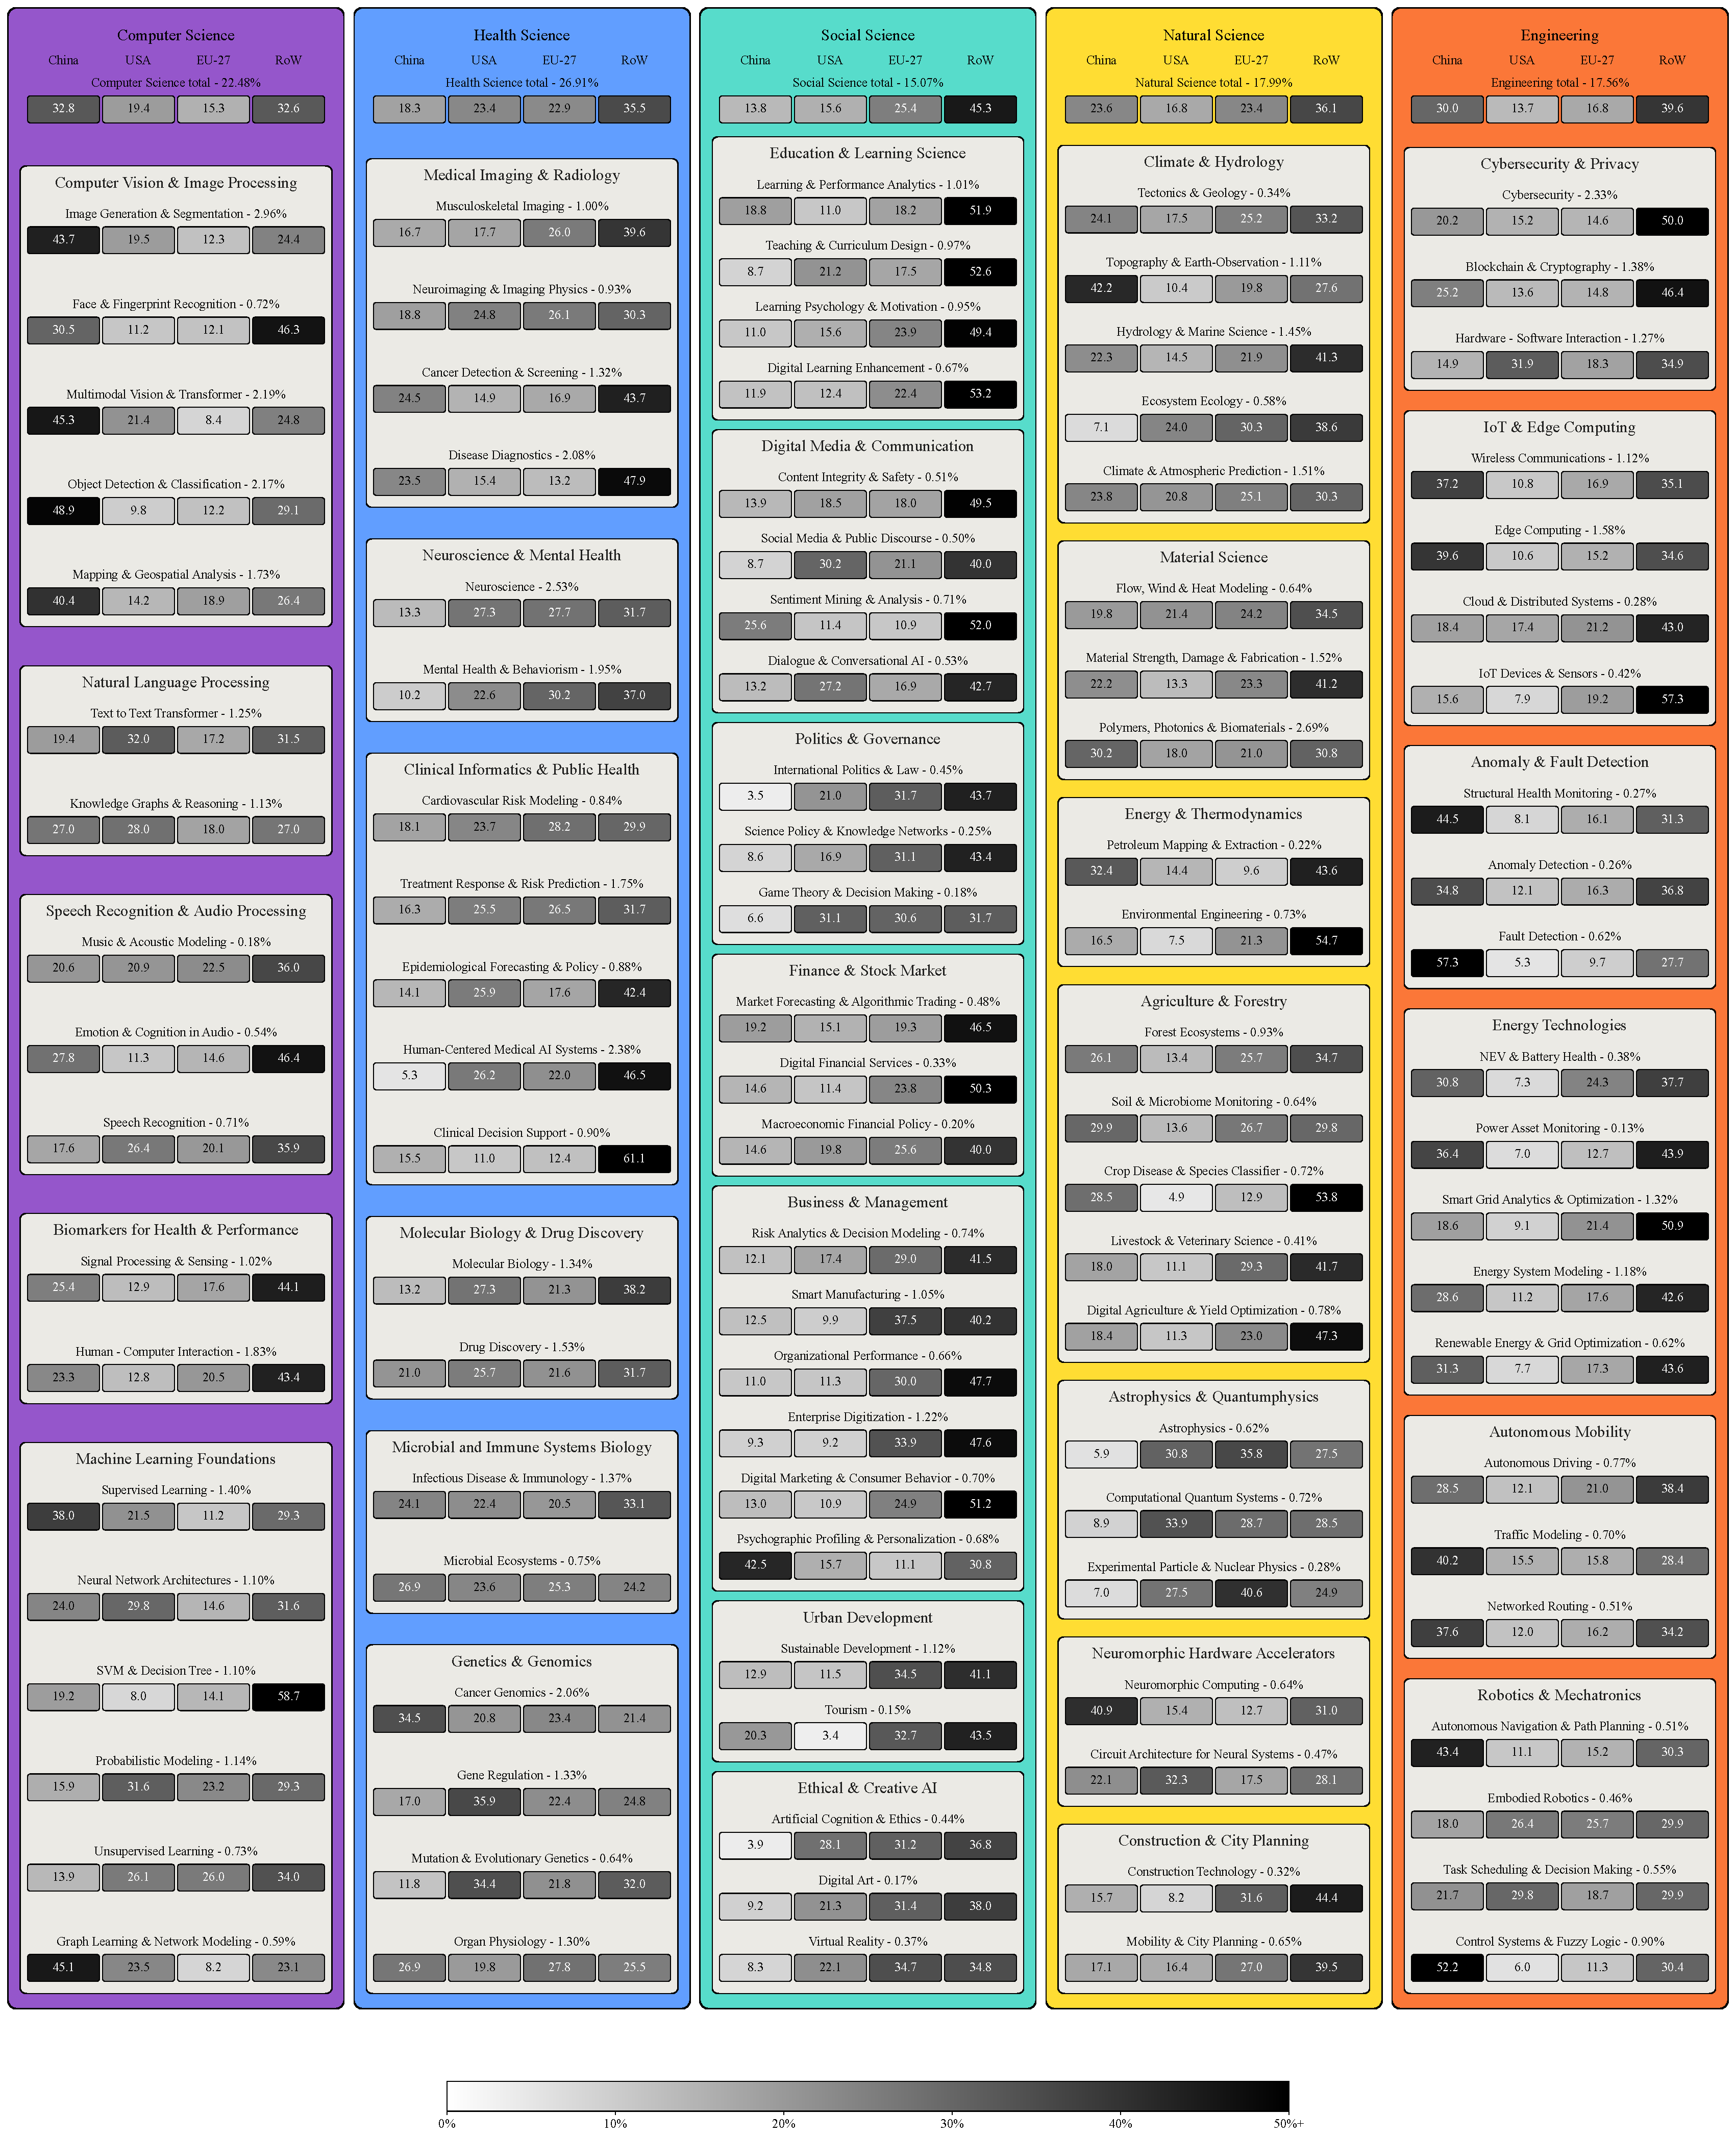
\includegraphics[width=\linewidth]{bloc_citation_shares_across_subdisciplines.pdf}
			\vspace{1em}
			\caption*{\small\textit{Figure 15 shows each bloc's shares of fractional citation sums across the 106 micro-clusters. Each column corresponds to one macro-domain, grouped into its meso- and micro-clusters sorted by their numeric identifier. The mini-heatmaps express the fractional citation shares of the blocs as well as the residual RoW-category with percentages overlaid. The color intensity encodes shares from zero to 50\%.}}
			\label{fig:topic_modeling_heatmap}
			\vspace{2em}
		\end{center}
	}]
	
	
	Beyond that China leads in \textbf{\texttt{Supervised Learning}} \microC{040} (38.02\%) and \textbf{\texttt{Graph Learning \& Network Modeling}} \microC{045} (45.13\%). In otherwise weak meso-clusters, China shows performative outliers in \textbf{\texttt{Psychographic Profiling \& Personalization}} \microS{245} (42.47\%), \textbf{\texttt{Topography \& Earth Observation}} \microN{301} (42.18\%), and \textbf{\texttt{Neuromorphic Computing}} \microN{350} (40.91\%). However, there are also many blindspots on the micro-level. Apart from the already known weaknesses on macro and meso-level China contributes remarkably little in \textbf{\texttt{Unsupervised Learning}} \microC{044} (13.87\%) and \textbf{\texttt{Ecosystem Ecology}} \microN{303} (7.11\%).
	
	\paragraph{USA:} The US combines 18.60\% of the citation share and leads the blocs in 1 of 5 macro-clusters, in 5 of 31 meso-clusters and in 22 of 106 micro-clusters. The US slightly leads in \textbf{\texttt{Health Science}} \microH{1} (23.36\%), ranks second behind China in \textbf{\texttt{Computer Science}} \microC{0} (19.38\%), and second behind the EU-27 in \textbf{\texttt{Social Science}} \microS{2} (15.56\%). At the same time the US is the last among the blocs in both \textbf{\texttt{Natural Science}} \microN{3} (16.83\%) and \textbf{\texttt{Enginnering}} \microE{4} (13.65\%).
	
	At the meso-level the US leads in \textbf{\texttt{Natural Langauge Processing}} \microC{01} (30.10\%), in \textbf{\texttt{Clinical Informatics \& Public Health}} \microH{12} (23.65\%), \textbf{\texttt{Genetics \& Genomics}} \microH{15} (25.93\%), in \textbf{\texttt{Molecular Biology \& Drug Discovery}} \microH{13} (26.46\%), and in \textbf{\texttt{Digital Media \& Communication}} \microS{21} (20.98\%). Just like China the US has significant weakpoints especially in \textbf{\texttt{Agricutlure \& Forestry}} \microN{33} (10.93\%), in \textbf{\texttt{IoT \& Edge Computing}} \microE{41} (10.88\%), \textbf{\texttt{Anomaly \& Fault Detection}} \microE{42} (7.48\%) and in \textbf{\texttt{Energy Technologies}} \microE{43} (9.28\%). 
	
	The Micro-level perspective makes that even more obvious. Here the US drops to single digits a total of 16 times, ranking last among the three blocs in 55 of 106 micro-clusters. Especially severe is the disadvantage in \textbf{\texttt{Object Detection \& Classification}} \microC{003} (9.77\%), \textbf{\texttt{SVM \& Decision Tree}} \microC{042} (8.00\%) and \textbf{\texttt{Control Systems \& Fuzzy Logic}} \microE{453} (6.03\%). Unforeseen strengths lie in \textbf{\texttt{Neural Network Architecture}} \microC{041} (29.76\%), \textbf{\texttt{Probabilistic Modeling}} \microC{043} (31.58\%), \textbf{\texttt{Game Theory \& Decision Making}} \microS{222} (31.08\%), \textbf{\texttt{Computational Quantum Systems}} \microN{341} (33.92\%), \textbf{\texttt{Hardware-Software Interaction}} \microE{402} (31.88\%), and \textbf{\texttt{Task Scheduling \& Decision Making}} \microE{452} (29.76\%).
	
	\paragraph{EU-27:} The EU-27 collectively contributes 20.79\% of total AI citations and demonstrates the most comprehensive disciplinary coverage among the three blocs. The EU-27 leads in 1 of 5 macro-clusters, in 9 of 31 meso-clusters and in 40 of 106 micro-clusters. The EU-27 leads in \textbf{\texttt{Social Science}} \microS{2} (25.38\%), ranks closely behind the US in \textbf{\texttt{Health Science}} \microH{1} (22.87\%), and closely behind China in \textbf{\texttt{Natural Science}} \microN{3} (23.45\%). However, in \textbf{\texttt{Computer Science}} \microC{0} (15.28\%) and \textbf{\texttt{Engineering}} \microE{4} (16.83\%), the EU-27 trails more substantially behind. 
	
	On the meso-level the European leadership is especially strong in \textbf{\texttt{Business \& Management}} \microS{24} (29.09\%), in \textbf{\texttt{Ethical \& Creative AI}} \microS{26} (32.57\%), and in \textbf{\texttt{Politics \& Governance}} \microS{22} (31.33\%). Beyond the social sciences the EU-27 leads in the following meso-clusters: \textbf{\texttt{Neuroscience \& Mental Health}} \microH{11} (28.75\%), \textbf{\texttt{Astrophysics \& Quantumphysics}} \microN{34} (33.48\%), and \textbf{\texttt{Construction \& City Planning}} \microN{36} (28.54\%). Weaknesses on the other hand can be seen in \textbf{\texttt{Computer Vision \& Image Processing}} \microC{00} (12.57\%), \textbf{\texttt{Natural Language Processing}} \microC{01} (17.56\%), and \textbf{\texttt{Machine Learning Foundation}} \microC{04} (16.10\%) but also in \textbf{\texttt{Cybersecurity \& Privacy}} \microE{40} (15.60\%).
	
	While that is about in line with what one would expect given the overall citation share, the observation of the micro-level is more remarkable. Only four micro-clusters fall below a 10\% citation share - \textbf{\texttt{Multimodal Vision \& Transformers}}, \microC{002} (8.39\%), \textbf{\texttt{Graph Learning \& Network Modeling}} \microC{045} (8.24\%), \textbf{\texttt{Petroleum Mapping \& Extraction}} \microN{320} (9.58\%), and \textbf{\texttt{Fault Detection}} \microE{422} (8.13\%) - significantly less than China (14) and the US (16). The EU-27's consistency is backed up by a low micro-cluster citation share standard deviation of 7.02\% in comparison to the US's 7.94\% and China's 11.77\%. Notable strengths on the micro-level can be found in \textbf{\texttt{Musculosceletal Imaging}} \microH{101} (26.01\%), \textbf{\texttt{Neuroimaging \& Imaging Physics}} \microH{102} (26.14\%), \textbf{\texttt{Ecosystem Ecology}} \microN{303} (30.29\%), and \textbf{\texttt{Livestock \& Veterinary Science}} \microN{333} (29.27\%).
	
	\paragraph{India:} Even though India is not explicitly represented in the shown graph, it is regularly considered an emergent powerhouse of AI research and will thus be covered here. On the macro-level, India is relatively consistens with 3.92\% in \textbf{\texttt{Computer Science}} \microC{0}, 3.25\% in \textbf{\texttt{Health Science}} \microH{1}, 4.13\% in \textbf{\texttt{Social Science}} \microS{2}, 4.09\% in \textbf{\texttt{Natural Science}} \microN{3}, and 4.92\% in \textbf{\texttt{Engineering}} \microE{4}.
	
	On the meso-level India shows the best performances in \textbf{\texttt{Agriculture \& Forestry}} \microN{33} (8.59\%), \textbf{\texttt{Digital Media \& Communication}} \microS{21} (8.50\%), \textbf{\texttt{Biomarkers for Health \& Performance}} \microC{03} (6.64\%), and \textbf{\texttt{Cybersecurity \& Privacy}} \microE{40} (6.55\%). The Lowest values can be found in \textbf{\texttt{Ethical \& Creative AI}} \microS{26} (1.31\%), \textbf{\texttt{Neuroscience \& Mental Health}} \microH{11} (1.32\%), and \textbf{\texttt{Genetics \& Genomics}} \microH{15} (1.32\%).
	
	On the micro-level India leads in one of the 106 clusters: \textbf{\texttt{Clinical Decision Support}} \microH{124} (15.94\%). Beyond that, India records its strongest performance in \textbf{\texttt{Crop Disease \& Species Cassifier}} \microN{332} (16.74\%), \textbf{\texttt{Digital Agriculture \& Yield Optimization}} \microN{334} (13.17\%), \textbf{\texttt{SVM \& Decision Tree}} \microC{042} (11.53\%), \textbf{\texttt{Content Integrity \& Safety}} \microS{210} (11.35\%), and \textbf{\texttt{Sentiment Mining \& Analysis}} \microS{212} (10.15\%). As indicated previously in the \nameref{performance_heatmap}, India ranks third in the national ranking of AI publication volume but lags substantially in citations per paper. Nevertheless, its research activity remains broad and comparatively even across subdisciplines, reflecting a extensive but still maturing scientific ecosystem. Overall India is a relevant actor in the AI research landscape yet it significantly trails the three blocs.
	
	\paragraph{The Rest of the World:} Even though the residual character of this entity might diminish its significance, it actually is the biggest of the five observed entities. Note that this category includes India. If it was included in the ranking of the three blocs, it would top 4 of 5 macro-clusters, 23 of 31 meso-clusters and in 77 of 106 micro-clusters with 36.51\% share of all citations. Yet one has to be realistic - even though the numbers are notable, there is too little institutional or political cohesion within this group of 164 countries. However, the observation of the category grants a different benefit: It shows which subdisciplines are most and least consolidated among the three blocs. On the macro-level the RoW category would lead in \textbf{\texttt{Health Science}} \microH{1} (35.52\%), \textbf{\texttt{Social Science}} \microS{2} (45.30\%), and \textbf{\texttt{Natural Science}} \microC{3} (36.09\%), and \textbf{\texttt{Engineering}} \microE{4} (39.56\%).
	
	On the meso-level especially large shares can be found in \textbf{\texttt{Speech Recognition \& Audio Processing}} \microC{02} (39.86\%), \textbf{\texttt{Biomarkers for Health \& Performance}} \microC{04} (43.68\%), \textbf{\texttt{Clinical Informatics \& Public Health}} \microH{12} (42.02\%), \textbf{\texttt{Energy \& Thermodynamics}} \microN{32} (52.19\%), \textbf{\texttt{Construction \& City Planning}} \microN{36} (41.11\%), \textbf{\texttt{Cybersecurity \& Privacy}} \microE{40} (45.16\%), and \textbf{\texttt{Energy Technologies}} \microE{43} (45.33\%). The lowest shares for RoW and thus the highest consolidation among the three blocs can be seen in the resource-intensive \textbf{\texttt{Genetics \& Genomics}} \microH{15} (24.52\%), \textbf{\texttt{Astrophysics \& Quantumphysics}} \microN{34} (27.47\%), and \textbf{\texttt{Robotics \& Mechatronics}} \microE{45} (30.16\%).
	
	On the micro-level, RoW would leads 77 of the 106 clusters. Only China, which leads 21 of the remaining 29 micro-clusters remains partly competitive due to its dominant performance in \textbf{\texttt{Engineering}} \microE{4} and \textbf{\texttt{Computer Science}} \microC{0}. But in \textbf{\texttt{Health Science}} \microH{1}, \textbf{\texttt{Social Science}} \microS{2}, and \textbf{\texttt{Natural Science}} \microN{3} RoW would take up 53 of 66 micro-clusters. Furthermore, RoW never falls below the 20\%-mark and drops below 25\% only seven times. 
	
	
	
	
	
	\subsubsection{Citation Share Subdiscipline Landscape}
	
	\figurename~\ref{fig:india_eu_usa_china_h3_citation_share} provides a more intuitive and accessible representation of the citation shares across subdisciplines. It allows to recognize patterns that remained undetected during the observation of the identified subdisciplines. The insights that are searched for within this graph are semantic regions with particularly high or low bloc citation shares. For that purpose, the two-dimensional UMAP topology introduced in the \nameref{subdiscipline_landscape} is reused, thereby preserving the spatial arrangement of research fronts while replacing the categorical color assignments of the established taxonomy with the jet color-scale to encode each bloc’s relative contribution to the total citation sum within every micro-cluster. Although the empirical distribution extends up to 57.3\% - observed for China in \textbf{\texttt{Fault \& Anomaly Detection}} \microE{422} - values above the 40\% threshold are clipped to ensure a balanced visual gradient across the majority of clusters. Also India is chosen over the RoW-bloc, largely to prevent the RoWs maxima from squishing other values on the lower half of the color-scale. The presented UMAP should be interpreted in conjunction with the legend and structural layout shown in legend of the \nameref{subdiscipline_landscape}, since the current figure depicts only the summarized topology without displaying individual micro-cluster labels. Note that findings that were already apparent from the numeric representation will not be repeated here.
	
	\paragraph{The EU-27's Only Weakness:} Until now, the EU-27 has mainly been praised for its high citation share consistency and stability across subdisciplines. However, some outliers can always be found - even among the social sciences, where Europe largely leads the blocs. There is, however, one semantic region whose low values are too widespread and consistent to be dismissed as outliers. The region concerned is the one surrounding the processing of visual data, which spans \textbf{\texttt{Computer Science}} \microC{0}, \textbf{\texttt{Health Science}} \microH{1}, and \textbf{\texttt{Natural Science}} \microN{3}. The EU-27 is not only lagging behind in the core area of \textbf{\texttt{Computer Vision \& Image Processing}} \microC{00}, but also in related methodological clusters such as \textbf{\texttt{Supervised Learning}} \microC{040} and \textbf{\texttt{Graph Learning \& Network Modeling}} \microC{045}, as well as in \textbf{\texttt{Disease Diagnostics}} \microH{103} and \textbf{\texttt{Clinical Decision Support}} \microH{124}.
	
	\paragraph{USA's Research Legacy:} As already established, the US shows greater variation across the semantic landscape of AI research. A concentration of high citation shares can be found in the region of \textbf{\texttt{Natural Language Processing}} \microC{01}, \textbf{\texttt{Machine Learning Foundations}} \microC{04}, and \textbf{\texttt{Neuroscience \& Mental Health}} \microH{11}. All of these are fields that were already relevant in the second AI summer of the 1990s \cite{nilsson_2009_quest_ai}. Outside of these traditional fields, the US lags well behind the EU-27 and China in many areas. This is particularly evident when looking at the blue rim surrounding these central fields and includes a large parts of \textbf{\texttt{Social Science}} \microS{2}, \textbf{\texttt{Natural Science}} \microN{3}, and \textbf{\texttt{Engineering}} \microE{4}. However, it would be too simplistic to portray the US as overall antiquated and backward. Traditional topics are still too central in 2025, and the US is too strong in the periphery of \textbf{\texttt{Natural Science}} \microN{3} and \textbf{\texttt{Health Science}} \microH{1} to support this claim. Yet this observation suggests that the US's leadership in these areas is a legacy of early research. Moreover it implies that ermerging areas of AI where demand is far from saturation and no revenue stream can shield American leadership from competitors, will be more fiercely contested internationally.
	
	\twocolumn[{%
		\begin{center}
			\captionof{figure}{Summarized UMAP of AI Subdisciplines by Bloc Citation Share}
			\vspace{1em}
			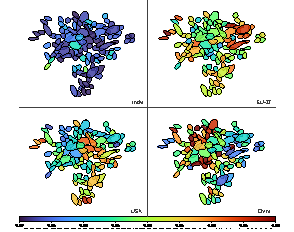
\includegraphics[width=\linewidth]{india_eu_usa_china_105_h3_cluster_comparison.pdf}		\label{fig:india_eu_usa_china_h3_citation_share}
			\vspace{1em}
			\caption*{\small\textit{Figure 16 presents the fractional citation shares of India, the EU-27, the US, and China across the micro-clusters. It reuses the summarized UMAP established earlier. The maximum of the color-scale is arbitrarily set to 40\%. To identify the names of individual clusters, the taxonomy of \nameref{subdiscipline_landscape} can be used.}}
			\vspace{2em}
		\end{center}
	}]
	
	\paragraph{China's Focal Points:} China owes its high averages primarily to two regions: The majority of \textbf{\texttt{Engineering}} \microE{4} and \textbf{\texttt{Computer Vision \& Image Processing}} \microC{00}. The former can be understood and explained as a spillover effect of China's undisputed production capacities. The latter, on the other hand, is difficult to explain by historical or economic path dependencies. Training with visual data is comparatively resource-intensive. In particular, large amounts of data and computing capacity are required. Leaner data protection and low infrastructure costs may have contributed to the success, but they cannot fully explain why China tends to be particularly strong in distinct subdisciplines. This pattern - or rather the absence of a clear pattern - is evident once again in the two outliers found in \textbf{\texttt{Graph Learning \& Network Modeling}} \microC{045}, as well as \textbf{\texttt{Profiling \& Personalization}} \microS{245}. Here, too, values are upwards of 40\%, without any spillover to semantic neighbors. What is particularly striking, are the high shares in robotics, computer vision, and control systems - a combination that could be summarized under the latest buzzword of technology enthusiasts: Embodied AI - the fusion of autonomous agents with the physical world. This phenomenon of seemingly \textit{unorganically grown} focal points of Chinese research might partly be explained by state-funded R\&D aiming at progress in fields of research that are considered strategic in extensive industrial policies like \textit{Made in China 2025} but their impact has yet to be thoroughly researched.
	
	
	\section{Caveats \& Limitations}
	\label{conclusion_limitations}
	
	Before addressing the research questions in the conclusion, it is imperative to acknowledge the inherent constraints of this study's data and methodology. The following section outlines key caveats and limitations, contextualizing the scope and interpretative boundaries of the scientometric analysis presented in this thesis.
	
	\paragraph{A Zero-Sum Game only by Research Design:} Because its in the nature of citation shares to sum up to 100\% within each cluster, research impact is inherently zero-sum in this study. In direct comparison one bloc’s strength is, by definition, another’s weakness. However, the premises of this rationale are disputed in international politics. While realists frame international competition in inherently zero-sum terms institutionalists and constructivists emphasize the potential for positive-sum outcomes through cooperation, division of labor, and rules-based global governance. Global academia has progressively agreed on a compromise that acknowledges the complexity of international politics and derives from it the necessity of a pluralistic, perhaps even eclectic perspective. In political practice, however - especially in matters of security - realistic views still prevail. This paper cannot and does not intend to make a prediction about the future prevalence of zero-sum logic, let alone an assessment of its appropriateness. It should merely be emphasized that the research design should in no way be misunderstood as an implicit endorsement of realistic security logic in the development of AI capacities.
	
	\paragraph{Scientometrics:} It is essential to recall the limitations inherent to scientometric analysis: (i) \textbf{Distortion by Goal-Setting:} Political and institutional incentives, along with evaluation systems that reward publication volumes, citation performances, or co-authorship rates can create artificial targets that distort genuine research behavior and impact measurement \cite{baccini2019citation, fire2018over}. (ii) \textbf{Ambiguity of Citation Meaning:} Citations serve heterogeneous and often ambiguous functions - ranging from acknowledgment of intellectual debt to contextual reference or even explicit criticism - thereby complicating their interpretation as indicators of scholarly influence \cite{adler2009citation, waltman2016review}. (iii) \textbf{Impact versus Visibility:} Citation counts frequently reflect patterns of visibility, prestige, and network centrality as much as, or even more than, genuine intellectual contribution \cite{waltman2016review}. (iv) \textbf{Structural Bias:} Scientometric data and global databases exhibit systematic biases favoring western, legacy, affluent, and anglophone institutions and authors, leading to a persistent imbalance in research visibility across and within countries \cite{Maddi2025GeographicalDisciplinaryCoverage, gomez2022leading}. (v) \textbf{Cumulative Advantage:} The Matthew effect implies that already highly-cited authors, journals, and institutions tend to accumulate citations at a disproportionate rate, producing a self-reinforcing cycle of visibility and recognition detached from intrinsic research quality \cite{wang2013quantifying, lariviere2009impact}.
	
	\paragraph{Topic Modeling:} The structure of topic models often reflects analytical design choices rather than intrinsic divisions within the data. Cluster boundaries are fragile and probabilistic, shaped by the selection of embedding models, dimensionality-reduction methods, and random initialization seeds. The hyperparameters governing these processes are not discovered from the corpus itself but deliberately tuned to enhance interpretability and thematic coherence from the standpoint of the operating scholar. Consequently, the resulting clusters should be understood as interpretive abstractions rather than objective reflections of linguistic or conceptual reality. Reproducibility in this context is therefore conditional rather than absolute: Small perturbations in parameter settings or random seeds can lead to markedly different cluster boundaries and label assignments. This uncertainty compounds in hierarchical models, where errors or ambiguities at higher levels propagate downward. For a modest percision of 90\% per layer, a three-tiered hierarchy would retain only about 72.9\% reliability (0.9\textsuperscript{3}), underscoring how uncertainty scales non-linearly with model depth. In this sense, topic modeling is best understood as a guided approximation of semantic space - an exploratory lens that aids interpretation, not a deterministic classifier of meaning.
	
	\paragraph{Temporal coverage:} Although examining the present offers immediacy and political relevance, temporal proximity limits analytical depth. The true trajectory and endurance of current developments can only be evaluated retrospectively, once their long-term significance has unfolded. Which of the works within the constructed dataset will remain influential for the decades to come remains to be seen. Citation-based indicators and topical salience at this stage represent informed conjectures rather than definitive assessments.
	
	Taken together, these caveats underscore that scientometric and computational analyses are never neutral mirrors of reality. Yet, there is ultimately no such thing as \textit{raw data} or the \textit{ideal method}: Every dataset, model, and hyperparameter carries its own simplifications and biases. A similar catalog of limitations could be created for any other empirical approach. Within these boundaries, however, the present study still offers a systematic, transparent, and analytically meaningful approximation of global AI research dynamics and is thus able to suggest some hypothesis on the research questions.
	
	\section{Conclusion}
	
	This thesis has explored the global landscape of research in artificial intelligence from 2020 to 2025 through a multi-layered scientometric analysis. Based on a comprehensive dataset from OpenAlex, a hierarchical taxonomy of AI subdisciplines was first developed using semi-supervised topic modeling. On this structural basis, the research impact of the most important national and international actors - in particular China, the US, and the EU-27 - was then analyzed on the global dataset and across subdisciplines. The key findings on the research questions are summarized below:
	
	\vspace{1em}
	\rule{\linewidth}{0.4pt}
	
	\begin{enumerate}
		\item[\textbf{RQ1}]\hspace*{2em}\parbox[t]{\dimexpr\linewidth-2em}{
			\textit{Which subdisciplines structure the contemporary AI research landscape?}
		}
	\end{enumerate}
	
	\vspace{0.25em}
	\rule{\linewidth}{0.4pt}
	\vspace{1em}
	
	\paragraph{Semantic Landscape of AI Research:} The hierarchical topic modeling subdivided the dataset into a semantic landscape that consists of 5 broad domains, 31 thematic fields, and 106 specialized research fronts. It revealed a clear core-periphery arrangement: The semantic core is represented by computer science, which combines the mathematical and methodological foundations, such as machine learning, neural networks, and computer vision. It is surrounded by four application-oriented domains: Health sciences, social sciences, natural sciences, and engineering, whose semantic distance from the core increases with their degree of domain specialization. This differentiated clustering highlights the problematic nature of the often-used simplistic view of AI as a uniform field and instead underscores its extraordinary thematic breadth and internal diversity. It is precisely this diversity that helps explain the marked fluctuations in national research impact profiles across subdisciplines.
	
	\paragraph{Public-Academic Attention Divergence:} Despite the underrepresentation of private-sector research suggested by the predominance of universities among the 100 most-cited institutions, research tends to concentrate on areas of application that are of commercial value. Most research is conducted in areas where financial incentives already exist. This is particularly the case where AI is not merely being tested but is already established as the best practice. A prime example of this is the subdiscipline of computer vision, which, together with its semantic neighbors - Radiology and Topography - accounts for a total of 16.21\% of the analyzed publications. By contrast, core public interests such as AI's ethical alignment and governance are only marginally represented in this study's dataset, accounting for a total of 2.7\%.  
	
	
	\paragraph{Periphery Growth Rates Outpace the Core:} An annual growth rate of 22.15\% across the entire dataset is contrasted with 14.74\% for computer science. In particular, core research areas such as machine learning, NLP, and robotics lag significantly behind health science, social science, and natural science. This pattern is partly attributable to the rapid diffusion of AI into new domains, where even modest absolute increases can translate into high percentage growth from initially low baselines. However, with growth rates in the core still remaining high when compared against total research production, it is too early to speak of an AI saturation in computer science. Rather, it can be said that low-hanging fruits can be found where there has traditionally been little involvement with computer science. This observation gives evidence to the hypothesis that AI functions as a general purpose technology that rapidly diffuses across all branches of science.
	
	\vspace{1em}
	\rule{\linewidth}{0.4pt}
	
	\begin{enumerate}
		\item[\textbf{RQ2}]\hspace*{2em}\parbox[t]{\dimexpr\linewidth-2em}{
			\textit{How are countries and blocs positioned within these subdisciplines in terms of their relative research impact?}
		}
	\end{enumerate}
	
	\vspace{0.25em}
	\rule{\linewidth}{0.4pt}
	\vspace{1em}
	
	\paragraph{Global Citation Distribution:} The assessment of fractional citation shares confirms the outstanding contribution of the three geo-economic blocs: China, the EU-27, and the US. Together, they account for 58.9\% of all publications and 63.5\% of all citations in the examined corpus. A population-weighted Gini coefficient of 0.665 for the citation distribution even exceeds the same metric for the global nominal GDP (0.632), confirming a stark geographical inequality in scientific influence. However, the analysis also shows that the growth rates of AI citations in the Global South (even without China) are more than twice as high as in the Global North, indicating a gradual reduction of inequality in the years to come.
	
	\paragraph{EU-27:} In contrast to its modest success in frontier model benchmarks and market capitalization, the EU-27 is one of the three pillars of AI research alongside China and the US, accounting for 20.79\% of global AI citations. Its strengths lie primarily in application-oriented domains: It leads in the social sciences, driven by fields such as economics, education, and politics. It is also strong in the health sciences and natural sciences, where it takes the lead in areas such as neuroscience, environmental science, and astrophysics. Relative weaknesses, on the other hand, are evident in the core methodological disciplines of computer science and engineering, particularly in subfields such as computer vision and machine learning. What makes the EU-27 stand out is its exceptional consistency. With the lowest standard deviation for citation shares across the 106 research fronts and only four fronts with single-digit shares, the EU-27 has the fewest thematic weaknesses or blind spots among the three blocs. This is also reflected in its institutional landscape: With 282 of the 1,000 most-cited institutions, the EU-27 has a broad, decentralized network of excellence. This European cluster is closely intertwined with US institutions in the co-authorship network, often mediated by British and Swiss nodes. In contrast, there is a greater distance to the Chinese cluster, which is separated by a belt of institutions from the rest of the world, reflecting the still comparatively low level of scientific networking between Europe and China. The EU-27s robust performance is particularly noteworthy considering that several high-performing non-EU countries - such as the UK, Switzerland, and Norway - are geographically and institutionally closest to the EU among the three observed blocs. Overall, public AI research in EU-27 countries shows competitive and robust performance, which definitely does not account for the poor European results in many other AI capacity metrics.
	
	\paragraph{China:} At 24.1\%, China accounts for the largest share of global AI citations among the three blocs. Its strengths are highly focused: China is the clear leader in the domains of computer science and engineering, with an outstanding position in clusters such as computer vision, anomaly detection, and robotics. In contrast, its weaknesses lie in the social sciences and health sciences, particularly in areas such as politics and clinical informatics. Remarkably, the Chinese profile shows relatively little continuity across the semantic landscape. In many cases, high citation rates are found right next to low ones. This extreme specialization is reflected in a comparatively high standard deviation across subdisciplines - maybe an indicator of a strategic focus on selected core technologies, while other fields are given significantly lower priority. The institutional landscape of the co-authorship network shows China's high level of domestic integration coupled with a relatively low level of international academic collaboration: China is home to 213 of the 1,000 most-cited institutions, but covers only a small part of the graph with a dense cluster insulated from the cluster of the US and the EU-27. A notable pattern is China's co-authorship proximity to geographical neighbors such as South Korea, Japan, and Australia. This finding underscores the strong influence of geographical, economic, and personal proximity over geopolitical alignment in scientific collaboration. Overall, the findings show that China has risen to become a powerhouse in AI research. Apart from significant blindspots in social science and parts of health science, China excels with high citation rates, primarily in areas of strategic importance to industry.
	
	
	\paragraph{USA:}The US contributes 18.60\% to global AI citations. Its strengths lie in health sciences, where it leads ahead of the EU-27 and China, as well as in historically established core areas of computer science. Machine learning, NLP, and neuroscience stand out in particular. However, there are also significant weaknesses in the domains of engineering and natural sciences, where the USA ranks a distant last among the blocs. It has particularly low citation shares in application-oriented fields such as agriculture, IoT, and energy technologies. This profile suggests that the US's leadership in \textit{legacy} subdisciplines - those that have been central since the second AI summer - remains strong. However, its competitiveness in most fields of application is significantly lower. This discrepancy is underscored by the lowest publication growth rate of all major economies. However, it should be noted that scientometric datasets only ever have access to public research. It therefore cannot be ruled out that there is a much higher proportion of private-sector research in the US. Overall, the performance of the US in the dataset stands in stark contrast to the dominance of proprietary AI models in benchmarks and the market valuations of its technology companies. This clearly shows that the development of AI has many layers.
	
	\paragraph{Citation Over- and Under-Performance:} An analysis of relative research performance - measured as the ratio of a country's share of global citations to its share of the global GDP - reveals clear patterns of overperformance and underperformance. The results vary greatly depending on which economic indicator is used as a basis. When research impact is measured against PPP-GDP, the biggest overperformers are predominantly small, highly developed economies. Countries such as Finland, Switzerland, and Denmark achieve many times the citation sums that would correspond to their economic weight. A completely different ranking emerges when the citation share is compared to nominal GDP. Here, countries of the Global South lead the list, with Iran at the top, followed by Pakistan, Malaysia, and Tunisia. Other remarkable achievements include the UK, which accounts for 6.96\% of the most-cited percentile of publications, the Netherlands, whose institutions make up seven of the ten most-cited institutions in the EU-27, and Australia, which contributes six institutions to the global top 100. At the other end of the scale, the two metrics agree in the identification of underperformers. Russia, Mexico, Brazil, and Japan show a citation share that lags far behind their respective economic weight. This finding is supported by their consistently low performance in most per-publication indicators, such as the average citation sum and the FWCI. 
	
	\section{Further Research}
	
	This thesis identifies key patterns in the global AI research landscape. At the same time, it reveals unanswered questions and areas that have not yet been sufficiently explored. In the following, research questions and topics that appear particularly relevant for future research are outlined. The aim is to highlight investigations that could help to deepen the understanding of scientometrics as a whole and the exploration of AI research in particular.
	
	
	\paragraph{Method-Domain Signal Separation:} Titles and abstracts encode both methodological and domain-specific vocabulary. They often co-occur in ways that blur the boundaries between epistemic innovation and applied context. Future research could apply linguistic disentanglement or dual-embedding models to explicitly separate methodological markers from domain identifiers. By modeling these components independently, subsequent clustering could minimize cross-domain noise and produce a clearer topology of methodological clusters.
	
	\paragraph{Within-Bloc Citations Filter:} The artificial inflation of citation counts (and other metrics) occurs predominantly among authors and institutions within the same research system. To avoid this bias, it could be interesting to measure institutions or countries by their ability to attract academic attention outside their bloc.
	
	\paragraph{Co-Authorship Correlation:} The neighborhood relationships among the 1,000 most-cited institutions raise the question of which indicators are the best for predicting international collaboration. Given how close some Australian and South Korean universities are to the China cluster, one should look beyond the usual suspects of cultural and political ties and also consider geography, foreign trade, and migration.
	
	
	
	\section{Data and Code}
	
	All code, and visualization developed for this thesis are accessible in the accompanying GitHub repository:
	
	\begin{center}
		\url{https://github.com/Pigeon-Effect/scientometric-analysis-of-ai-research}
	\end{center}
	
	The repository contains the complete Python implementation for data retrieval from OpenAlex, topic modeling, citation analysis, and figure generation.
	
	\newpage
	\onecolumn
	\section{Glossary}
	
	
	\begin{table}[htbp]
		\centering
		\begin{threeparttable}
			\vspace{2em}
			\label{tab:glossary}
			\small
			{\color{darkgray}
				\begin{tabular*}{\textwidth}{@{\extracolsep{\fill}}ll}
					\textbf{Term} & \textbf{Definition}\vspace{0.5em}\\
					\hline
					\noalign{\vskip 0.5em}
					AI & \textbf{A}rtificial \textbf{I}ntelligence. \\
					ASEAN & \textbf{A}ssociation of \textbf{S}outh-\textbf{E}ast \textbf{A}sian \textbf{N}ations. \\
					Blocs & China, the EU-27, and the USA. \\
					BRICS & \textbf{B}razil, \textbf{R}ussia, \textbf{I}ndia, \textbf{C}hina, \textbf{S}outh Africa. \\				
					CAGR & \textbf{C}ompound \textbf{A}nnual \textbf{G}rowth \textbf{R}ate. \\
					CNN & \textbf{C}onvolutional \textbf{N}eural \textbf{N}etwork. \\
					DNN & \textbf{D}eep \textbf{N}eural \textbf{N}etwork. \\
					EU-27 & European Union after the United Kingdom’s withdrawal (post-2020). \\
					EU-28 & European Union before the United Kingdom’s withdrawal (2013-2019). \\
					EU-44 & All countries geographically attributed to Europe. \\
					FWCI & \textbf{F}ield-\textbf{W}eighted \textbf{C}itation \textbf{I}mpact. \\
					GCC & \textbf{G}ulf \textbf{C}ooperation \textbf{C}ouncil. \\
					GDP & \textbf{G}ross \textbf{D}omestic \textbf{P}roduct. \\
					GPT & \textbf{G}enerative \textbf{P}re-Trained \textbf{T}ransformer. \\
					G-77 & \textbf{G}roup of \textbf{77} - coalition of the Global South. \\
					IGO & \textbf{I}nter-\textbf{G}overnmental \textbf{O}rganization. \\
					IoT & \textbf{I}nternet of \textbf{T}hings. \\
					K-Means & Unsupervised clustering algorithm minimizing within-cluster variance. \\
					LLM & \textbf{L}arge \textbf{L}anguage \textbf{M}odel. \\
					LSTM & \textbf{L}ong \textbf{S}hort \textbf{T}erm \textbf{M}emory. \\
					Macro, Meso, Micro & Three labeling granularities of the topic modeling. \\
					Mercosur & Southern Common Market - South American trade bloc. \\
					MRI & \textbf{M}agnetic \textbf{R}esonance \textbf{I}maging. \\
					NLG & \textbf{N}atural \textbf{L}anguage \textbf{G}eneration. \\
					NLP & \textbf{N}atural \textbf{L}anguage \textbf{P}rocessing. \\
					OECD & \textbf{O}rganisation for \textbf{E}conomic \textbf{C}o-Operation and \textbf{D}evelopment. \\
					PPP & \textbf{P}urchasing \textbf{P}ower \textbf{P}arity adjusted. \\				
					ROAD & Directory of Open Access Scholarly Resources. \\
					RoW & The \textbf{R}est \textbf{o}f the \textbf{W}orld - all countries outside the \textit{blocs}. \\
					R\&D & \textbf{R}esearch and \textbf{D}evelopment. \\
					SKG & \textbf{S}cientific \textbf{K}nowledge \textbf{G}raph. \\
					SPECTER & \textbf{S}cientific \textbf{P}aper \textbf{E}mbeddings using \textbf{C}itation-informed \textbf{T}ransform\textbf{ER}s. \\
					TF-IDF & \textbf{T}erm \textbf{F}requency - \textbf{I}nverse \textbf{D}ocument \textbf{F}requency. \\
					UMAP & \textbf{U}niform \textbf{M}anifold \textbf{A}pproximation and \textbf{P}rojection. \vspace{0.5em} \\
					
					\hline
				\end{tabular*}
			}
			\vspace{1em}
		\end{threeparttable}
		\vspace{1em}
	\end{table}
	
	
	
	\clearpage
	\twocolumn
	
	\section{References}
	
	\printbibliography[heading=none]
\end{document}